% Preamble
% ---

\documentclass{article}



% Packages
% ---

\newcommand\ChangeRT[1]{\noalign{\hrule height #1}}
\usepackage{amsmath}
%\usepackage{verbatim}
\usepackage{graphicx}
\usepackage{url}

\renewcommand{\baselinestretch}{1.5}   
\usepackage[margin=1.5in] {geometry}
\renewcommand{\labelitemi}{$\bullet$} 

\usepackage{indentfirst}
\setlength{\parindent}{1.5cm}
\setlength{\parskip}{1em}


\title{TRAVEL REPORT}
\author{Yu Hsiang Chang, 103282001 \\
National Central University (NCU), Taoyuan City, Taiwan (R.O.C)}
\date{February 1 - July 31, 2017}

\begin{document}

\maketitle

\newpage

\tableofcontents
\listoffigures
\listoftables

\newpage





\section{Introduction}
In February 1 to July 31 of 2017, I was send by NCU to stay at the European Organization for Nuclear Research (CERN) to do my PhD studies, which is near the Geneva Swizterland and located in the boundary between France and Swizterland.    

During these time, I worked for my analysis ``Search for Z' to ZH to llbb with 2016 CMS data'' and participant the CMS future upgrade project ``High Granularity Calorimeter(HGCal)''. Beside these two tasks, I was also assigned a task for JMAR group as the service work and took shift of CMS trigger shift for 2017 data taking.

This traval report is the summary of these four activities.     

%

%\begin{comment}

\section{Search for Z' to ZH to llbb with 2016 CMS data}
Continuing the work in later 2016, I used 2016 CMS data to search the new particle Z', which decayed to a Z boson and a Higgs, and then the Z decayed to two leptons (electrons or muons pair) and the Higgs decayed to two b-quarks. 

The dataset used is listed in the Table 1, and the total luminosity = 34.14 fb$^{-1}$. The simulated Monte Carlo(MC) used is listed in the Table 2. The event selection is summarized in the Table 3. One can find more detail in \cite{Alberto ZH paper with 2015 data}. 

The following subsections describe my progresses in six months.

\begin{table}[]
\caption{dataset used for 2016}
\label{my-label}
\centering
\setlength{\tabcolsep}{8pt}
\begin{tabular}{ c }
\textbf{dateset name}     \\ \ChangeRT{1.5pt}
\hline
/SingleMuon/Run2016B-23Sep2016-v3/MINIAOD \\
/SingleMuon/Run2016C-23Sep2016-v3/MINIAOD \\
/SingleMuon/Run2016D-23Sep2016-v3/MINIAOD \\
/SingleMuon/Run2016E-23Sep2016-v3/MINIAOD \\
/SingleMuon/Run2016F-23Sep2016-v3/MINIAOD \\
/SingleMuon/Run2016G-23Sep2016-v3/MINIAOD \\
/SingleMuon/Run2016H-PromptReco-v2/MINIAOD \\
/SingleMuon/Run2016H-PromptReco-v3/MINIAOD \\ \hline
/SingleElectron/Run2016B-23Sep2016-v3/MINIAOD \\
/SingleElectron/Run2016C-23Sep2016-v3/MINIAOD \\
/SingleElectron/Run2016D-23Sep2016-v3/MINIAOD \\
/SingleElectron/Run2016E-23Sep2016-v3/MINIAOD \\
/SingleElectron/Run2016F-23Sep2016-v3/MINIAOD \\
/SingleElectron/Run2016G-23Sep2016-v3/MINIAOD \\
/SingleElectron/Run2016H-PromptReco-v2/MINIAOD \\
/SingleElectron/Run2016H-PromptReco-v3/MINIAOD \\ \hline
    
\end{tabular}
\end{table}



\begin{table}[]
\caption{MC sample used 2016, the ``*'' are for different mass points or H$_{T}$ values}
\label{my-label}
\centering
\setlength{\tabcolsep}{8pt}
\begin{tabular}{ c }
\textbf{MC sample name}     \\ \ChangeRT{1.5pt}
\hline

ZprimeToZhToZlephbb\_narrow\_M-*\_13TeV-madgraph \\
DYJetsToLL\_M-50\_TuneCUETP8M1\_13TeV-amcatnloFXFX-pythia8 \\
DYJetsToLL\_M-50\_HT-*to*\_TuneCUETP8M1\_13TeV-madgraphMLM-pythia8 \\
TT\_TuneCUETP8M2T4\_13TeV-powheg-pythia8 \\
ZZ\_TuneCUETP8M1\_13TeV-pythia8 \\
WZ\_TuneCUETP8M1\_13TeV-pythia8 \\
WW\_TuneCUETP8M1\_13TeV-pythia8 \\
ZH\_HToBB\_ZToLL\_M125\_13TeV\_amcatnloFXFX\_madspin\_pythia8 \\
ZH\_HToBB\_ZToLL\_M125\_13TeV\_powheg\_pythia8 \\

\end{tabular}
\end{table}


\begin{table}[]
\caption{event selection, the ``*'' are for different version. The data filter and noise cleaning haven't been applied here. The ``same'' means the same cut muon is applied on the muon channel as on the eletron channel.}
\label{my-label}
\centering
\setlength{\tabcolsep}{8pt}
\begin{tabular}{ c c c }
\textbf{ }      &  \textbf {electron channel} & \textbf{muon channel}     \\ \ChangeRT{1.5pt}
\hline
data filter     & { \_ } 		      & { \_ } \\
trigger         & HLT\_Ele105\_CaloIdVT\_GsfTrkIdT\_v*  & HLT\_Mu45\_eta2p1\_v* \\
nVtx            & { \textgreater= 1} 	      & {same } \\
\hline 
\textbf {lepton}& { } 			      & { } \\   
ID     		& { two loose } 	      & { one HighPt and one Custom tracker } \\
Iso    		& { already in ID} 	      & { trackerIso\textless0.1} \\
p$_{t}$     		& { \textgreater135,20}       & { \textgreater55,20} \\
$\eta$    	& $|\eta|$  \textless2.4, no 1.4442\textless$|\eta|$\textless1.566  & { $|\eta|$\textless2.4} \\
\hline 
\textbf {Z boson} & { } 		      & { } \\ 
p$_{t}$   	   	& { \textgreater200} 	      & { same} \\
mass 	   	& { 70\textless mass \textless200} & { same } \\
\hline 
\textbf {Higgs AK8 jet} & { } 	    	      & { } \\
ID              & { one loose } 	      & { same } \\
lepton cleaning & { no jet overlapped in      $\Delta$R\textless0.8 } & { same } \\
p$_{t}$              & { \textgreater200} 	      & same \\
$\eta$          & $|\eta|$  \textless2.4      & same \\
Soft Drop mass  & { 105\textless SDmass \textless135 } & { same } \\
b-tagging       & { Double B-tagger\textgreater0.3} & {same } \\
\hline
noise cleaning  & { \_ } 		      & { \_ } \\

\end{tabular}
\end{table}



\subsection{MC/data comparison}

The MC/data comparison was performed to make sure our understanding of physics is correct. 

A pre-selection, which was the same to event selection but without the double B-tagger cut and revised the Soft Drop mass to be \textless 65 or \textgreater 135 (the 65\textless Soft Drop mass \textless105 was also blinded for W/Z boson region), was applied for MC/data comparison.  

The results of the Z boson and the Higgs jet's transverse momentum (p$_{t}$) and the mass in the muon channel are showed in Figure 1. The results in the electron channel are simialr to the muon channel. 

Although the MC/data comparisons were not perfect, but since the final background estimation (see Sec. 2.3 ) did not rely on MC, the MC was still acceptable to use in later studies.


\begin{figure}
\centering
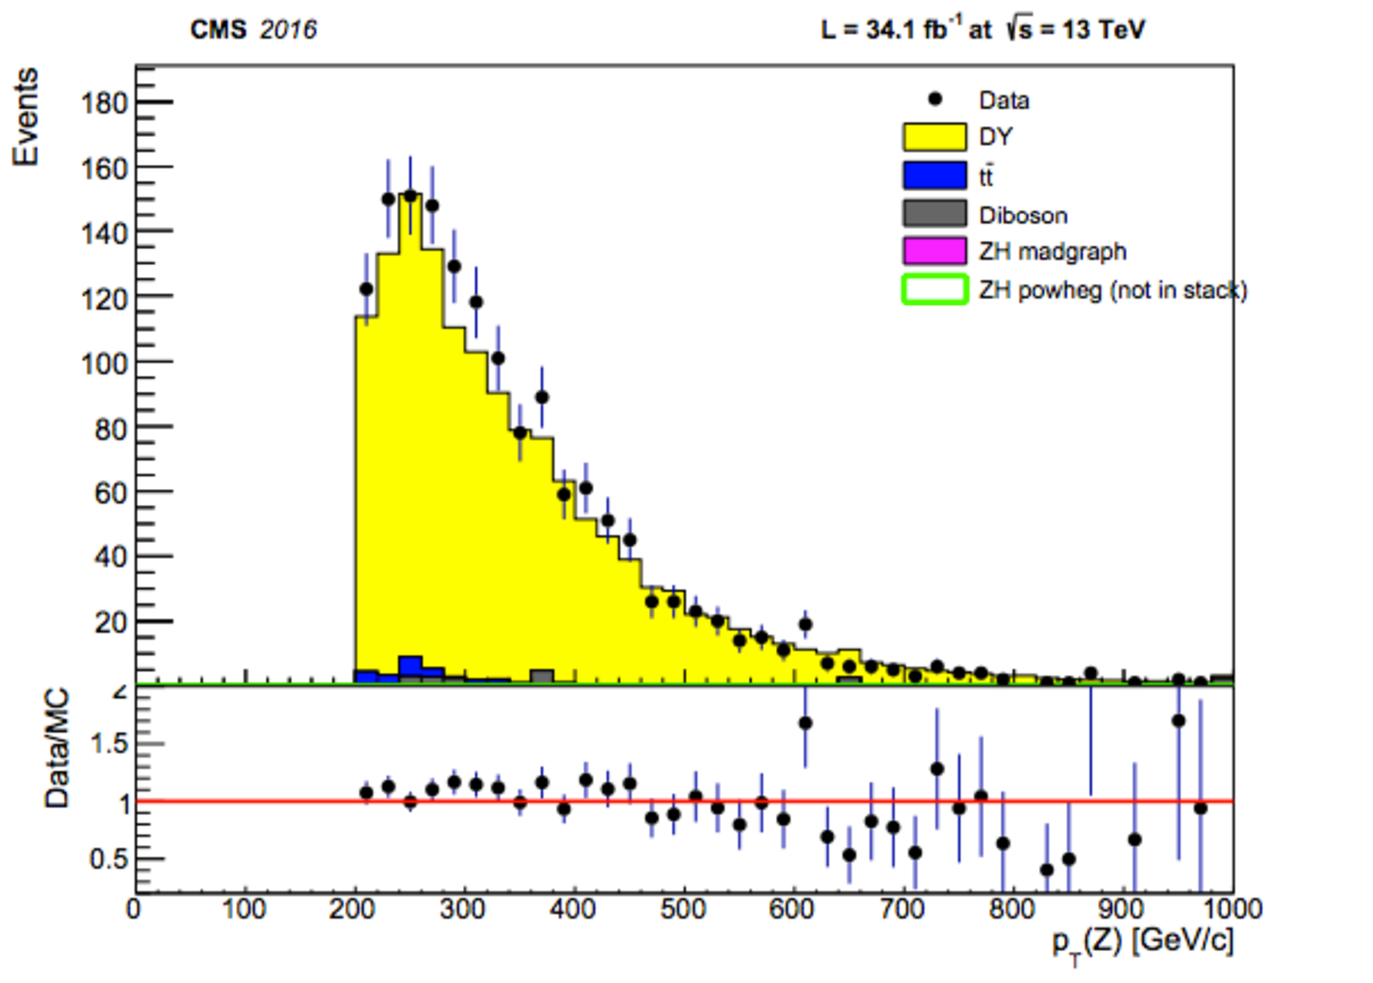
\includegraphics[width=.45\textwidth]{figures/mu_Zpt.pdf}\quad
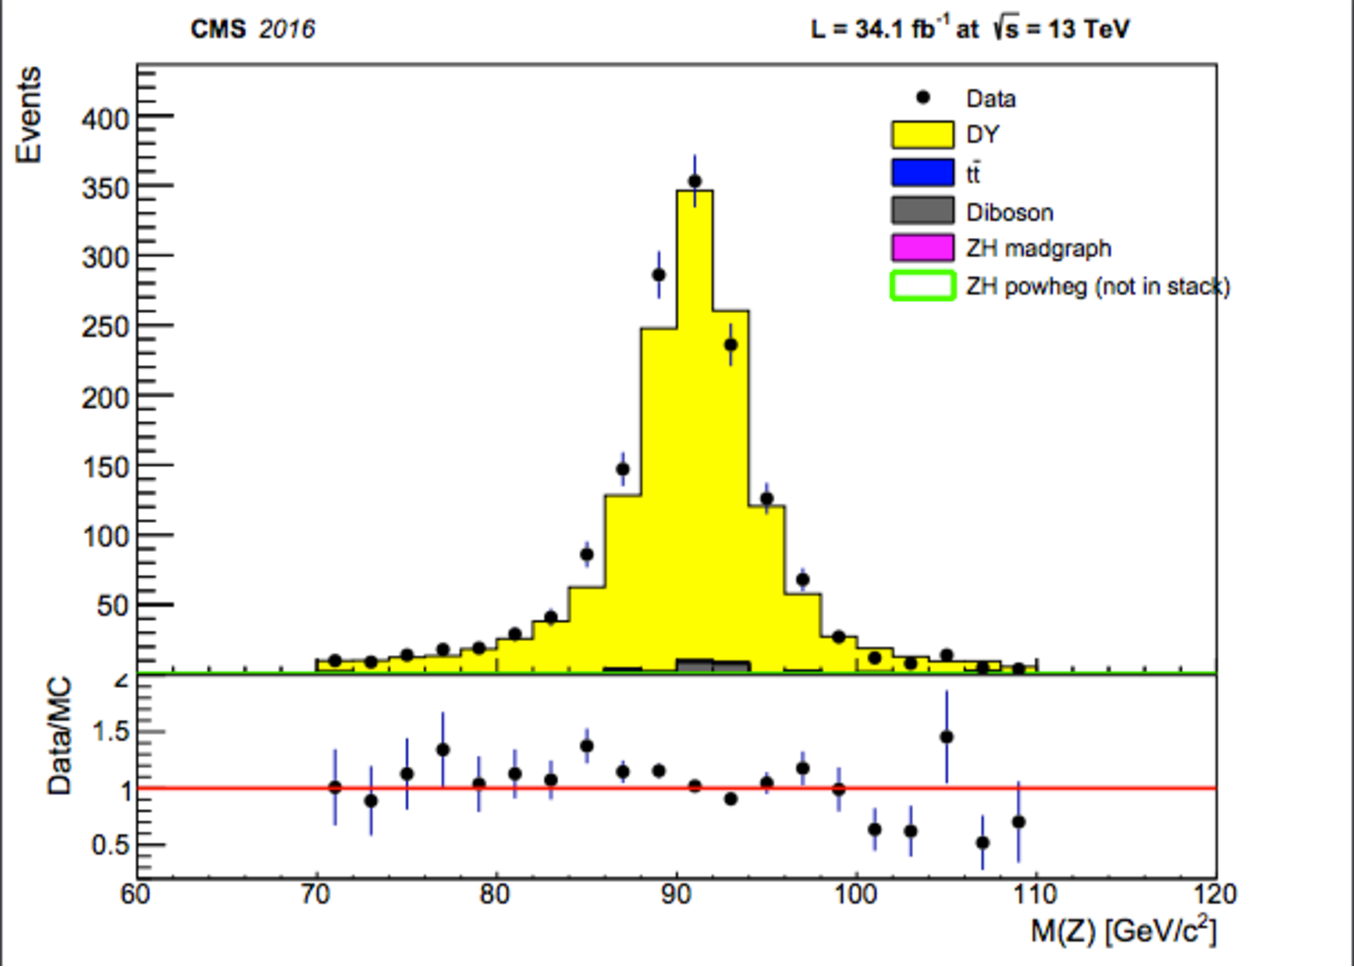
\includegraphics[width=.45\textwidth]{figures/mu_Zmass.pdf}
\medskip
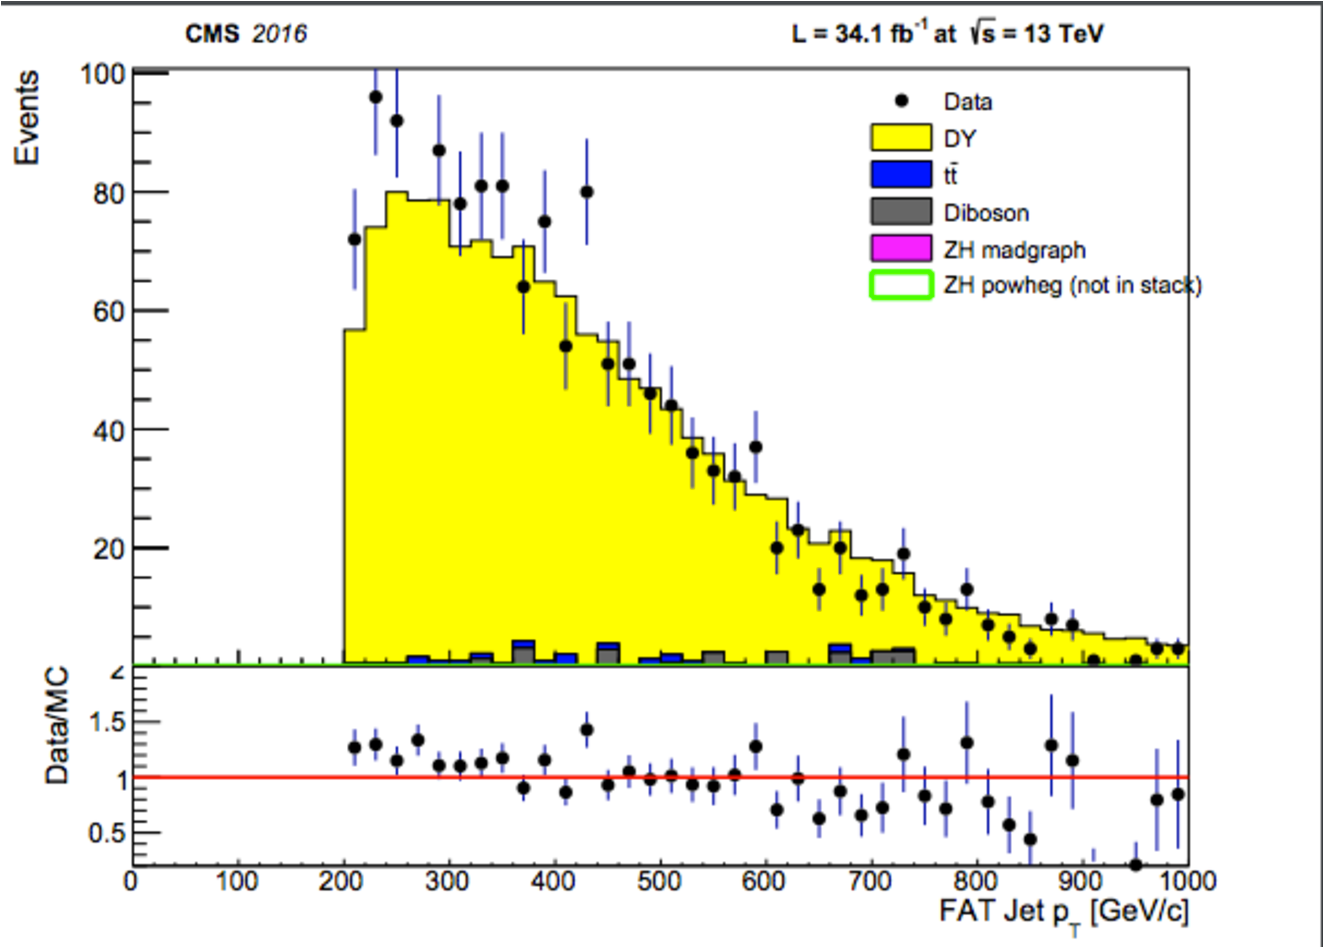
\includegraphics[width=.45\textwidth]{figures/mu_Jetpt.pdf}\quad
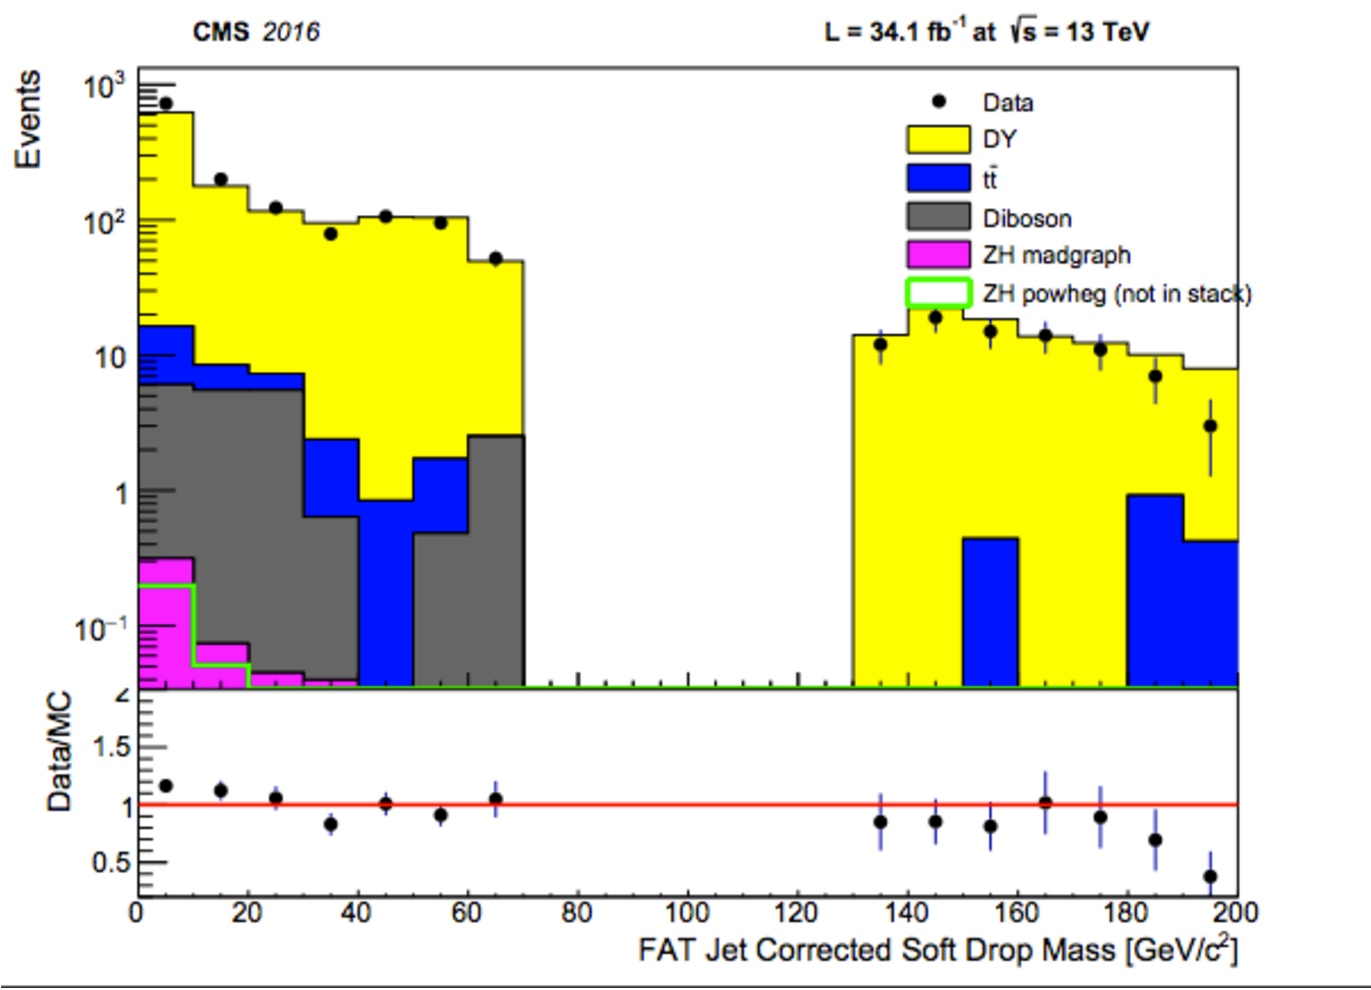
\includegraphics[width=.45\textwidth]{figures/mu_JetSDmass.pdf}
\caption{The MC/data comparison of the muon channel in the Z p$_{t}$(top left), the Z mass(top right), the fat jet p$_{t}$(bottom left) and the fat jet Soft Drop mass(bottom right).}
\label{pics:blablabla}
\end{figure}



\subsection{Double B Tagger Scale Factor}

The double B-tagger is an algorithm used to identify the fat jet containing two b-quarks \cite{double B-tagger paper}. For every comparison between data and MC in the certain cut, the MC must be applied this cut's scale factor(SF) to cover the difference in efficicy to data. This subsection describes the applying double B-tagger's SF to MC/data comparison.

In general, the formula of the event weight could be more complicated when the event has more than one jets passing double B-tagger, but since this analysis only has one jet, each event just times the SF as the event weight of double B-tagger.

There are two SFs depending on the jet passing double B-tagger belonged to the signal topology (H to bb) or background topology (ttbar) \cite{double B-tagger SF twiki}. The values of two kinds of SFs are listed in Table 4.

In this analysis, a fat jet tagged as b-quark and it has at least one subjet tagged as b-quark in the MC truth was considered as the signal topology, while a fat jet tagged as other (c-quark or u,d,s-quark or gluon) was considered as the background topology.
  
The MC/data comparison after applying the pre-selection, the double B-tagger cut and its SF is showed in Figure 2.


\begin{table}[]
\caption{Double B-tagger's scale factor}
\label{my-label}
\centering
\setlength{\tabcolsep}{8pt}
\begin{tabular}{ c c c c c c}
\textbf {signal topology} & {}    & {}      & {}      & {}      & {}              \\ 
p$_{t}$ bin                    & 0-250 & 250-350 & 350-430 & 430-840 & \textgreater840 \\ 
SF                        & 0.96  & 0.96    & 1.00    & 1.01    & 1.01            \\ \ChangeRT{1.5pt}
\hline
\textbf {background topology} & {}    & {}      & {}      & {}      & {}              \\
p$_{t}$ bin                        & 0-250 & 250-350 & 350-430 & 430-700 & \textgreater700 \\ 
SF                            & 1.044 & 1.044   & 1.074   & 1.119   & 1.119           \\
\end{tabular}
\end{table}


\begin{figure}
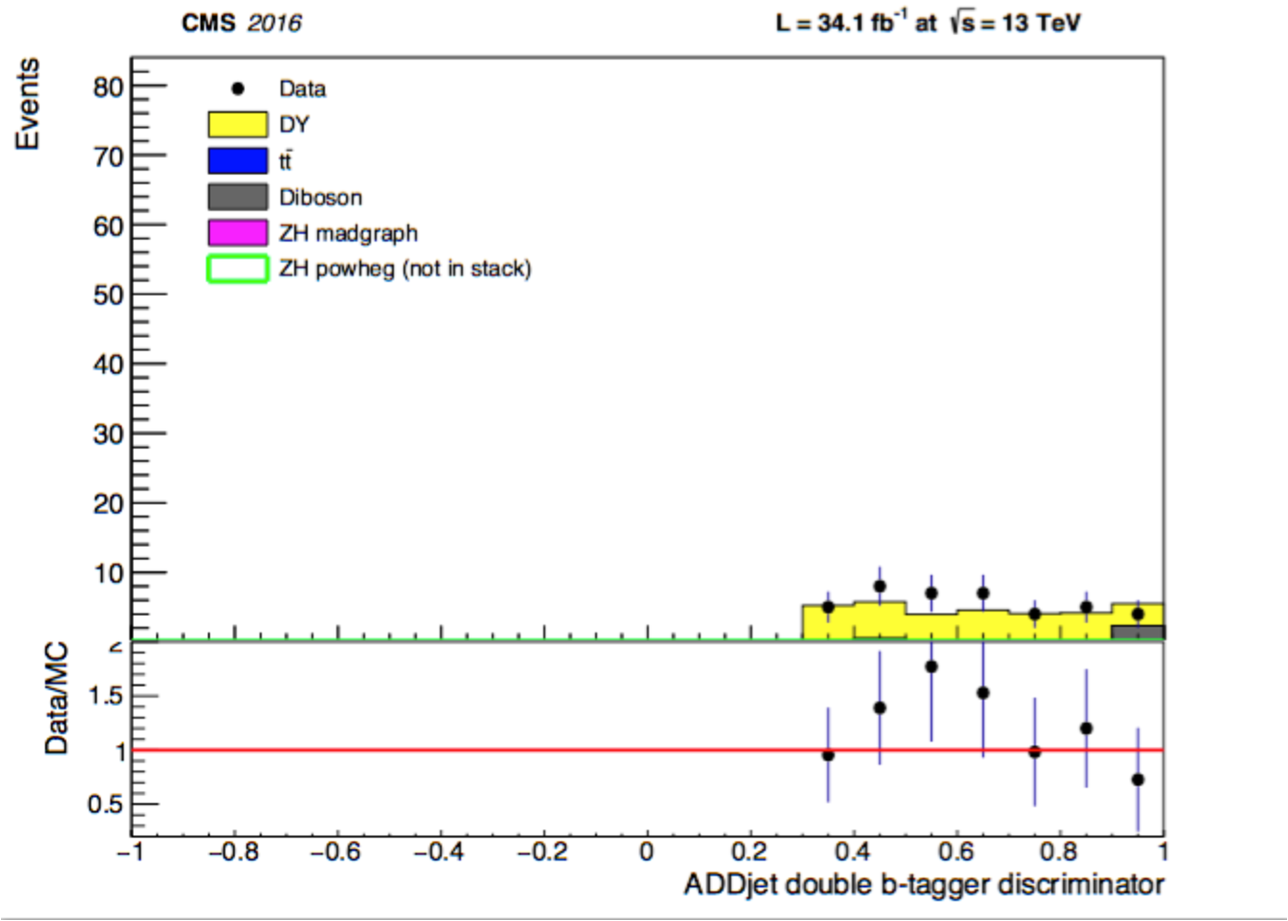
\includegraphics[width=.7\textwidth]{figures/doubleB_appliedSF.pdf}
\centering
\caption{The MC/data comparison in double B-tagger after applying the scale factor}
\label{pics:blablabla}
\end{figure}



\subsection{Estimating background by ALPHABET method}

The ALPHABET method is to use the events in data failing the double B-tagger to predict the event passing double B-tagger in Soft Drop mass window ( 105\textless SDmass \textless135 ). In the assumption that the double B-tagger and the Soft Drop mass have no correlation, one can fit the pass/fail double B-tagger event ratio in the left and right sidebands of the Soft Drop mass window then extrapolate the fit function to the mass window. Therefore, with the events failing double B-tagger and the pass/fail ratio description in the mass window, one can predict the events passing the double B-tagger and in the Soft Drop mass window, which is our final signal region(SR).    

To increase the statistics, the electron channel and the muon channel were combined together. 

This method could be validated by performing the same precedure in a control sample in data by requesting tau21\textgreater 0.4, which was assumed with negligible signal events, and then opening events passing double B-tagger and in the mass window to compare the true events and the predicted events. The passing and failing events in Soft Drop mass distribution is shown in Figure 3. The pass/fail ratio in the Soft Drop mass and the predicted and the true Zh invariant mass distribution are shown in Figure 4. The fit function for pass/fail ratio is the second order polynoimal (see Eqn. 1).  

\begin{equation}
y=p_{0}\cdot x^{2}+p_{1}\cdot x+p_{2}
\end{equation}

The difference between the true and the predicted events in the tau21 control sample is around 9\%, which is not big so there is potentials to use this method.

The pass/fail ratio in the Soft Drop mass and the predicted Zh invariant mass in the search sample (the data containing the real signal region) are shown in Figure 5. The events in signal region are blinded here.


\begin{figure}
\centering
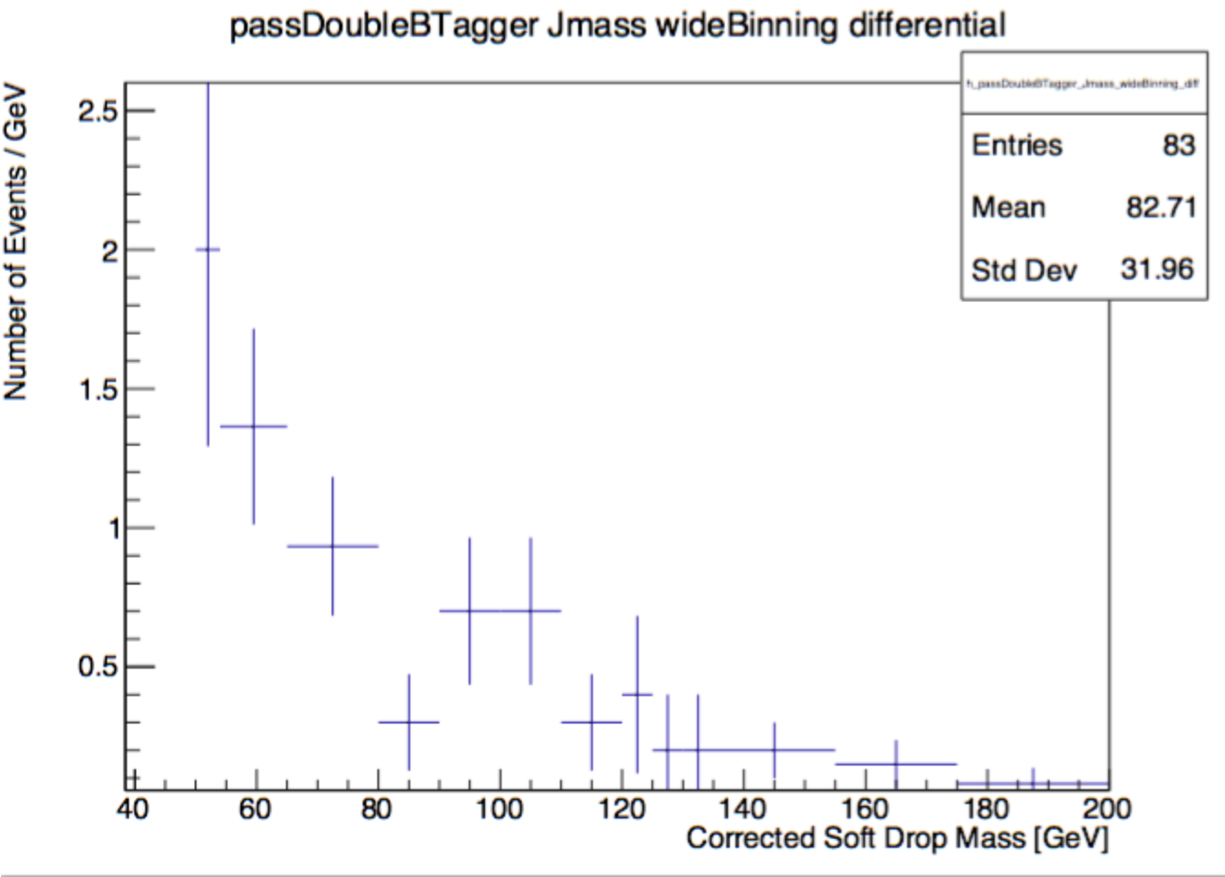
\includegraphics[width=.45\textwidth]{figures/tau21Region_Pass.pdf}\quad
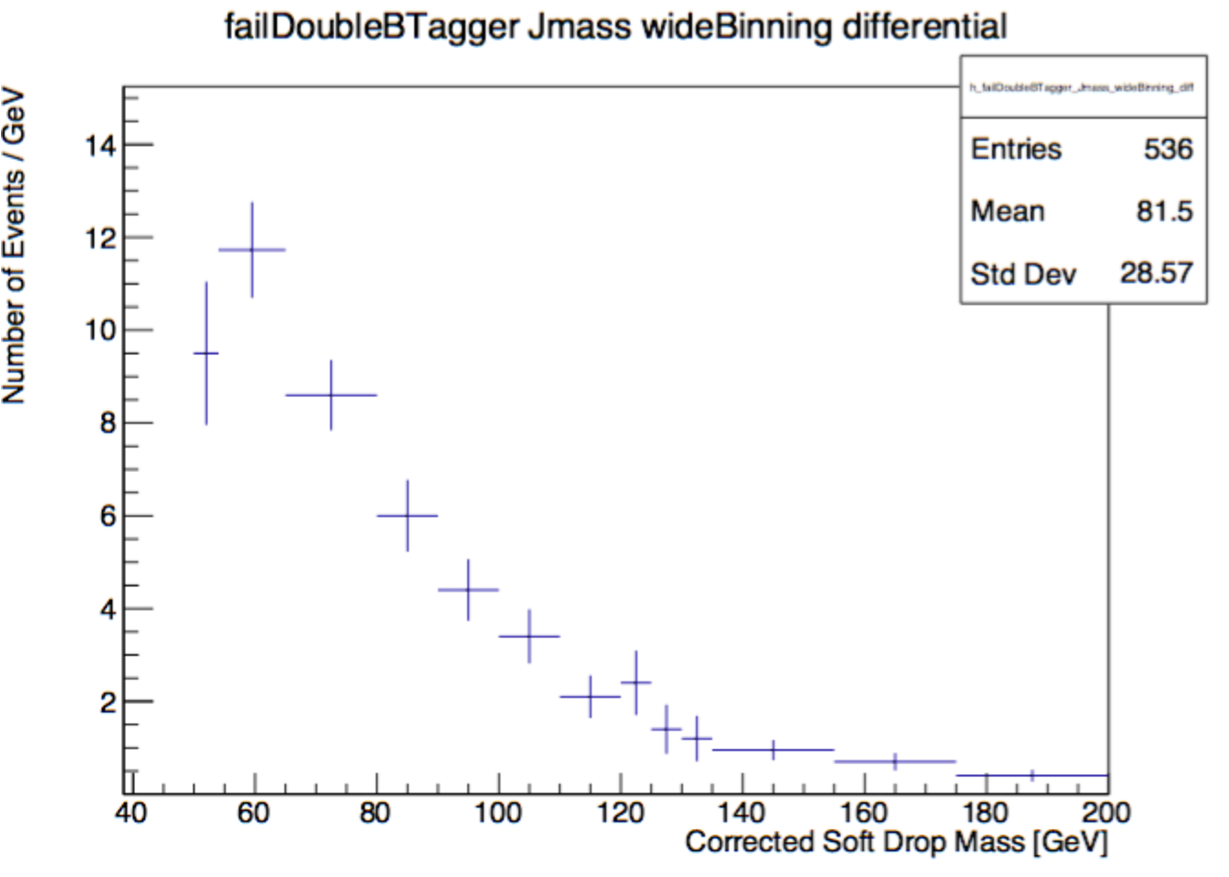
\includegraphics[width=.45\textwidth]{figures/tau21Region_Fail.pdf}
\caption{In tau21 control sample, the Soft Drop mass distributions passing double B-tagger(left) and failing double B-tagger(right)}
\label{pics:blablabla}
\end{figure}


\begin{figure}
\centering
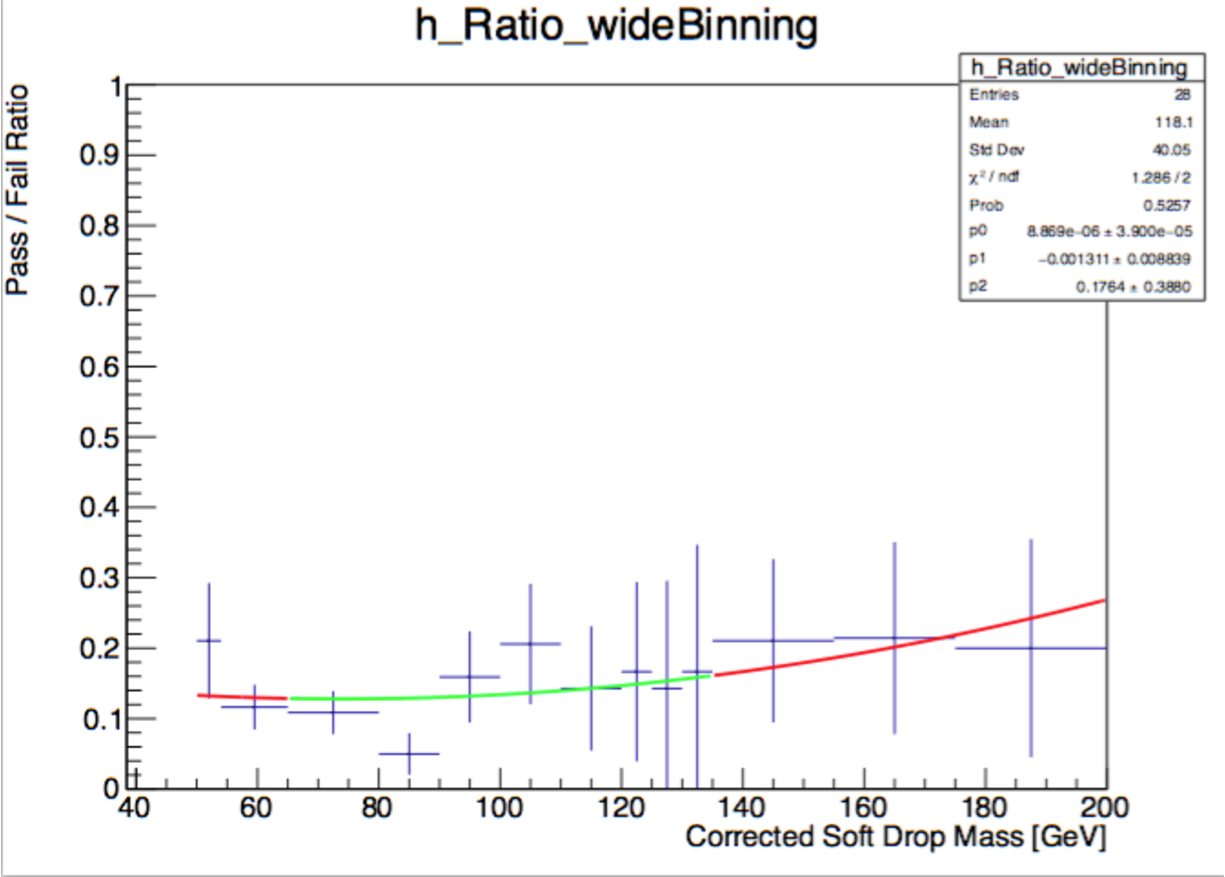
\includegraphics[width=.45\textwidth]{figures/tau21Region_PassFailRatio.pdf}\quad
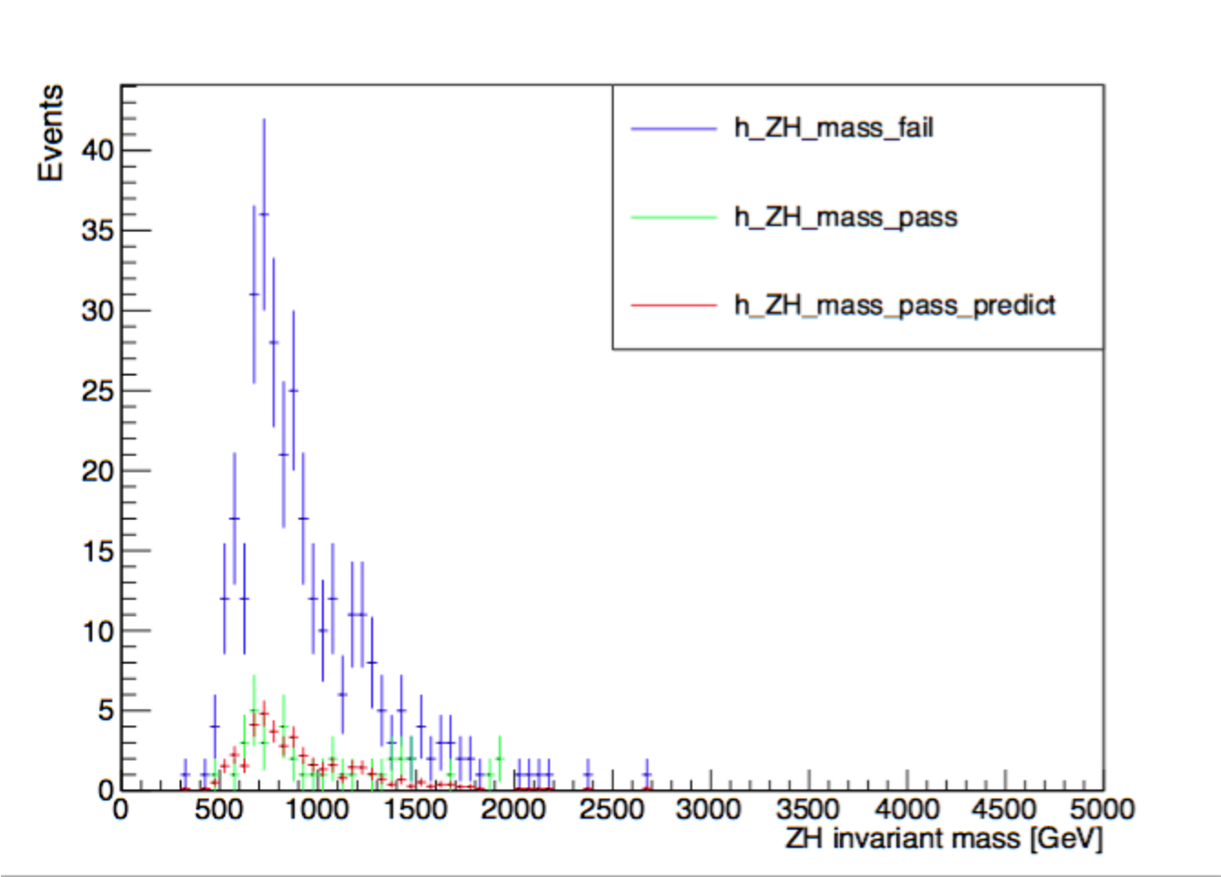
\includegraphics[width=.45\textwidth]{figures/tau21Region_ZHmass.pdf}
\caption{In tau21 control sample, the pass/fail ratio in Soft Drop mass(left) and the comparison of failing double B-tagger, true passing double B-tagger and predicted double B-tagger in the ZH invariant mass(right)}
\label{pics:blablabla}
\end{figure}



\begin{figure}
\centering
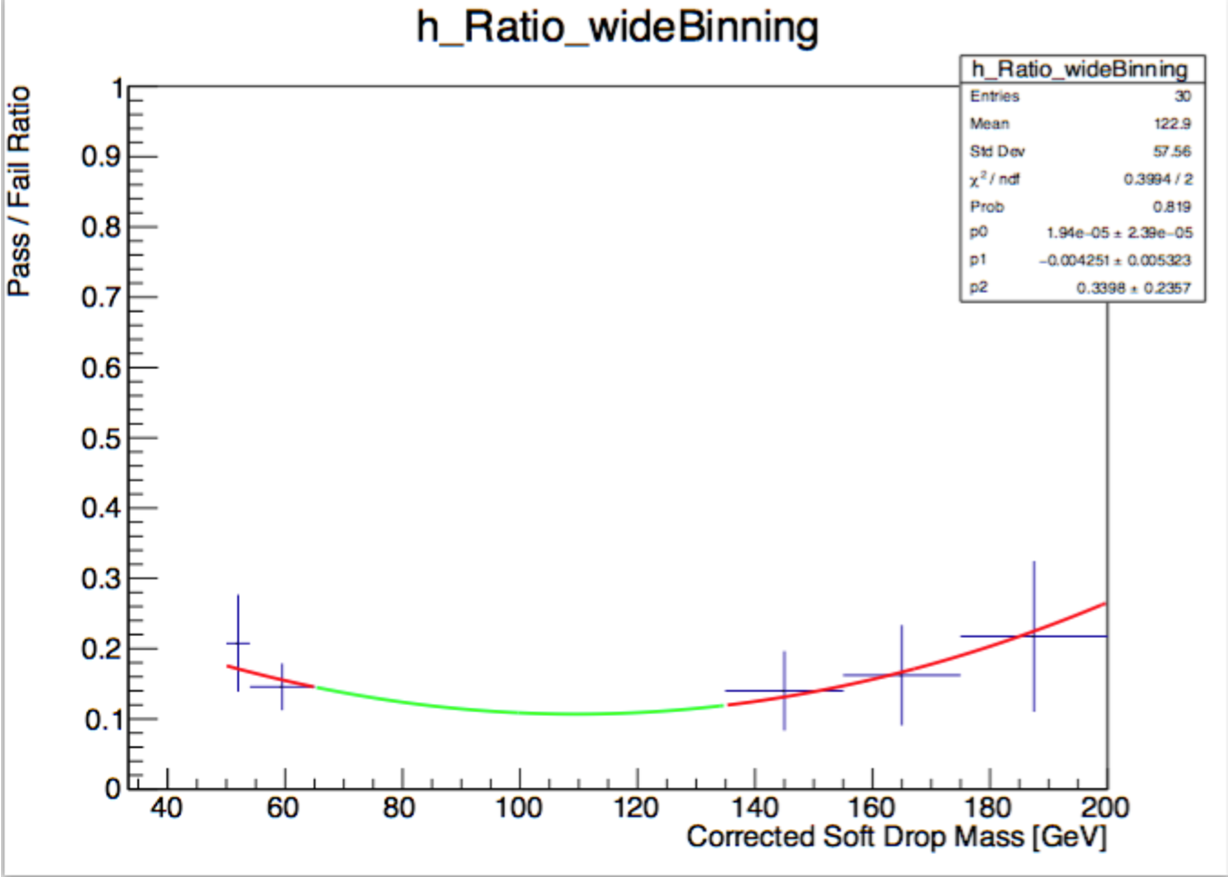
\includegraphics[width=.45\textwidth]{figures/SRRegion_PassFailRatio.pdf}\quad
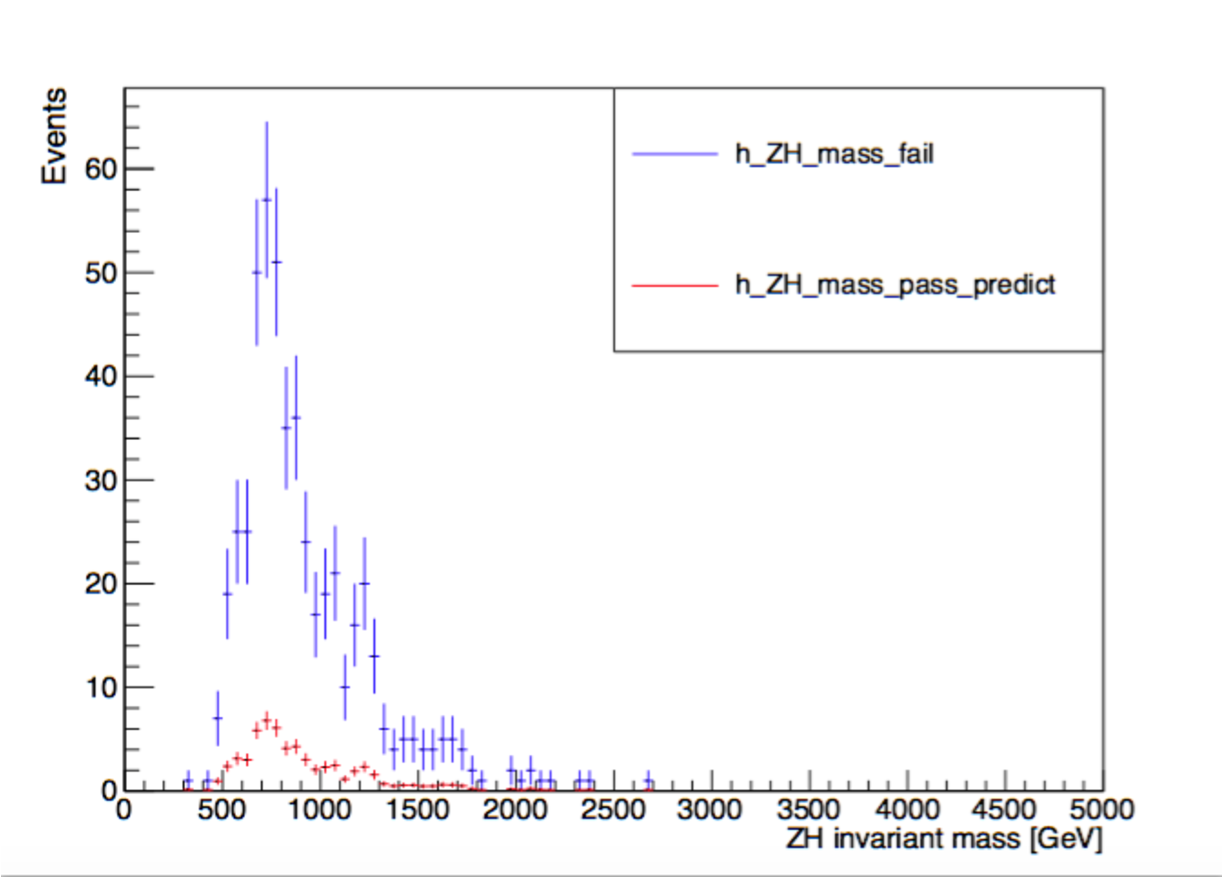
\includegraphics[width=.45\textwidth]{figures/SRRegion_ZHmass.pdf}
\caption{In search sample, the pass/fail ratio in Soft Drop mass(left) and the comparison of failing double B-tagger, true passing double B-tagger and predicted double B-tagger in the ZH invariant mass(right)}
\label{pics:blablabla}
\end{figure}

\subsection{Signal contanmination in the tau21 control sample}

In previous subsection the validation in the tau21 control sample is shown, which is in the assumption that negligible or no signal events passing double B-tagger and in the mass window. So this subsection is for answering that if there is signal contanmination then how it affects the validation.   

The tau21 distributions in the muon channel of the signal sample at different mass points are shown in Figure 6. Each signal sample is scaled to data luminosity = 34.1 fb$^{-1}$.  

The signal sample at mass = 1000 GeV is taken as the benchmark to compare with the backgrounds (dominated by DY sample), because it has more events after scaling. The tau21 distribution of the signal, the DY and the combined are shown in Figure 7. The signal fraction in tau21 \textgreater 0.4 is 7.6\% when the signal sample at mass = 1000GeV exists. And in this case the presencce of 7.6\% signal fraction could change the difference between predicted background and true background (data events substracts the signal contanimation) from original 9\% to 17.9\%, as shown in Eqn. 2. The N is the data events passing double B-tagger and in mass window, and the calculation is in the case that predict events \textgreater original true events (the opposite case does not changes the maximum difference).

\begin{equation}
\textup{maximum difference}=\frac{(N\times 1.09-N\times 0.924)}{N\times 0.924}=17.9\%
\end{equation}


If the signal does exist, the  maximum differences in the tau21 control sample for validation are listed in Table 5. 


\begin{table}[]
\caption{signal contamination and maximum difference}
\label{my-label}
\centering
\setlength{\tabcolsep}{8pt}
\begin{tabular}{ c | c c c c c c c c c c}
mass point            & 1000  & 1200  & 1400  & 1600  & 1800  & 2000  & 2500 & 3000         & 3500         & 4000         \\
\hline
signal contanmination & 7.8\% & 7.6\% & 5.2\% & 3.9\% & 2.2\% & 1.5\% & 1\%  & \textless1\% & \textless1\% & \textless1\% \\ 
\hline
maximum difference    & 17.9\%  & 14\%  & 13\%  & 11\%  & 10\%  & 9\%   & 9\%  & 9\%          & 9\%          & 9\%          \\

\end{tabular}
\end{table}



\begin{figure}
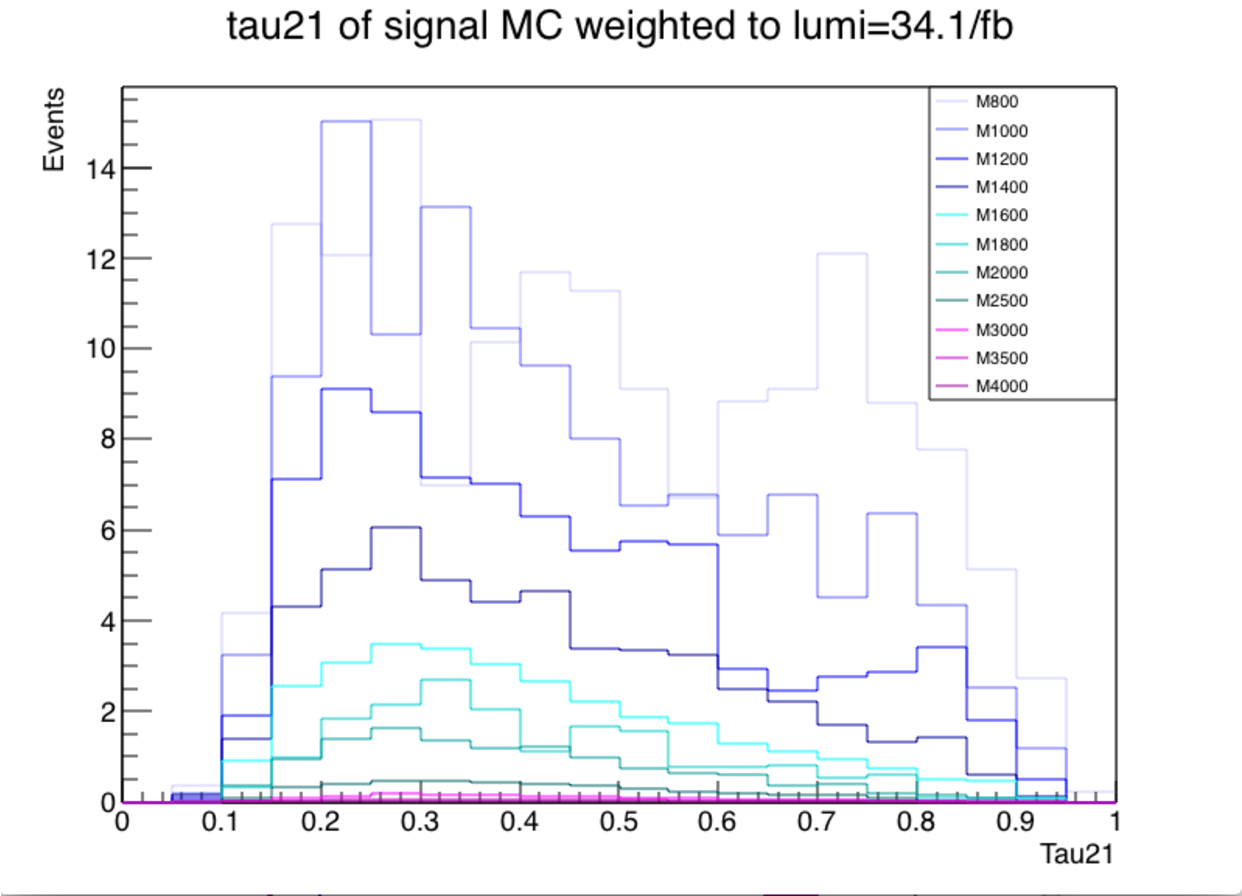
\includegraphics[width=.7\textwidth]{figures/tau21_SignalSample.pdf}
\centering
\caption{The tau21 distribution of signal samples at different mass points. The pre-selection has been applied.  }
\label{pics:blablabla}
\end{figure}



\begin{figure}
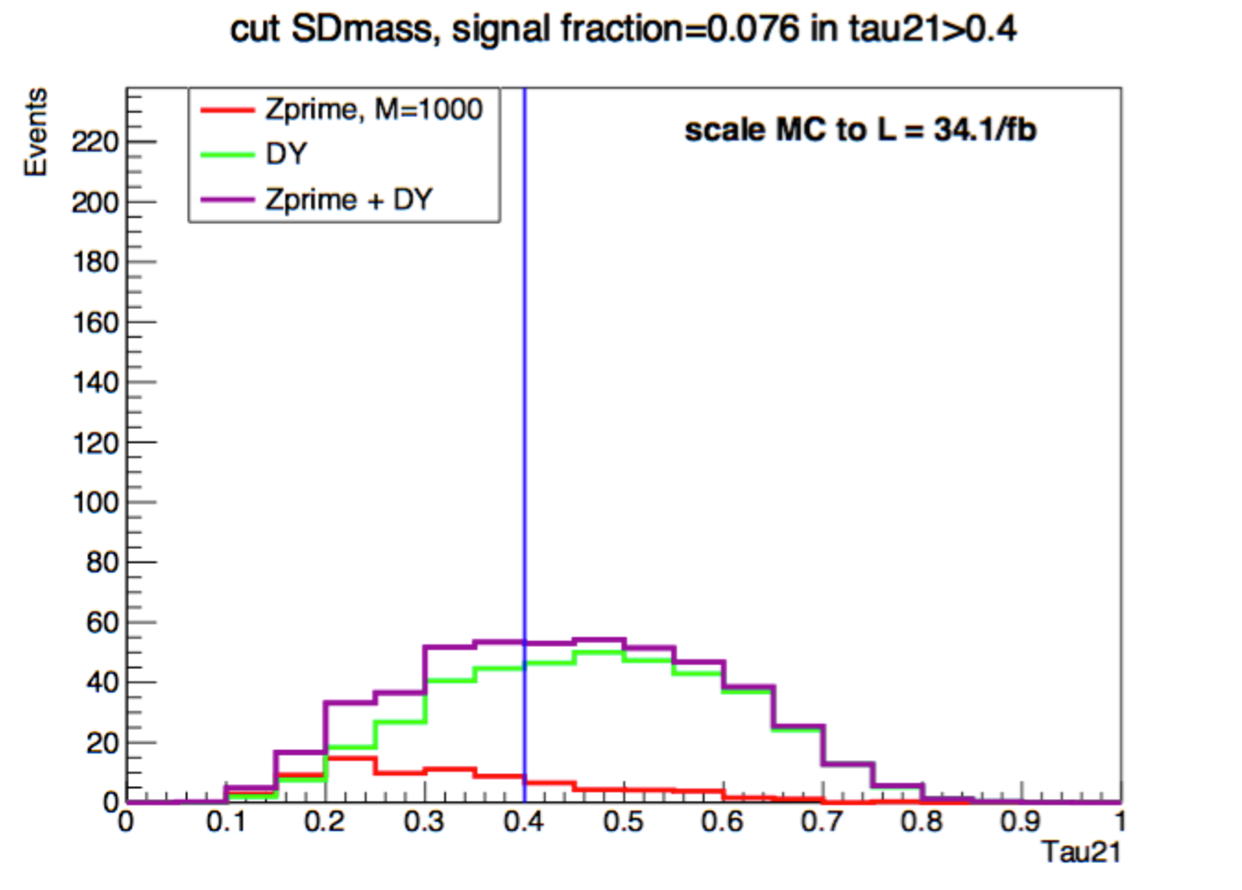
\includegraphics[width=.7\textwidth]{figures/tau21_SignalBackgroundSample.pdf}
\centering
\caption{The tau21 distribution of signal at mass point = 1000 GeV(red), DY background(green), and the combined(purple).}
\label{pics:blablabla}
\end{figure}


\subsection{The DY sample cross section correction K-factor}

In this analysis, four DY H$_{T}$-binned samples (100-200, 200-400, 400-600, 600-Infinity, the 600-Infinity is combined by other higher H$_{T}$-binned samples) are used for simulation studies, where the H$_{T}$ is the scalar sum of hadron p$_{t}$ in the LHE level. However, the cross section of H$_{T}$-binned samples is in the leading order (LO) only. To describe the DY process more preciously to the next leading order(NLO), one need to derive the correction k-factors for each DY H$_{T}$-binned samples's cross sections.

To derive the k-factors, one need to compare the NLO DY sample and the sum of each LO DY H$_{T}$-binned samples in the generator-level Z boson p$_{t}$(gen-Z p$_{t}$) distribution when all samples are scaled to the same luminosity, and this is indeed equivalent to solve four linear equations with four unknowns as shown in Eqn. 3. The $k_{i}$ is the k-factor for each DY H$_{T}$-binned sample, and the subscripts i=1,2,3,4 correspond to four LO H$_{T}$ binned samples 100-200, 200-400, 400-600, 600-Infinity respectively. The coefficients $x^{j}$ correspond to the normalization of four samples (a,b,c,d) and NLO DY sample (e), and the superscripts j=1,2,3,4 correspond to four generator-level Z boson p$_{t}$ ranges 100-200, 200-400, 400-600, 600-Infinity respectively.   

\begin{equation}
\begin{split}
k_{1}\cdot a^{1}+k_{2}\cdot b^{1}+k_{3}\cdot c^{1}+k_{4}\cdot d^{1}=e^{1} \\ 
k_{1}\cdot a^{2}+k_{2}\cdot b^{2}+k_{3}\cdot c^{2}+k_{4}\cdot d^{2}=e^{2} \\ 
k_{1}\cdot a^{3}+k_{2}\cdot b^{3}+k_{3}\cdot c^{3}+k_{4}\cdot d^{3}=e^{3} \\ 
k_{1}\cdot a^{4}+k_{2}\cdot b^{4}+k_{3}\cdot c^{4}+k_{4}\cdot d^{4}=e^{4} \\ 
\end{split}
\end{equation}

Since the gen-Z p$_{t}$ will drop very rapid in the right edge of the H$_{T}$, the equations can be reduced to the easier one in Eqn.4 (the bottom-left parts of the off-diagonal line are zero). 

\begin{equation}
\begin{split}
k_{1}\cdot a^{1}+k_{2}\cdot b^{1}+k_{3}\cdot c^{1}+k_{4}\cdot d^{1}=e^{1} \\ 
k_{1}\cdot 0    +k_{2}\cdot b^{2}+k_{3}\cdot c^{2}+k_{4}\cdot d^{2}=e^{2} \\ 
k_{1}\cdot 0    +k_{2}\cdot 0    +k_{3}\cdot c^{3}+k_{4}\cdot d^{3}=e^{3} \\ 
k_{1}\cdot 0    +k_{2}\cdot 0    +k_{3}\cdot 0    +k_{4}\cdot d^{4}=e^{4} \\ 
\end{split}
\end{equation}

The derived k-factors are listed in Table 6, and the gen-Z p$_{t}$ distributions of before and of after applying k-factors are shown in Figure 8. To be consistent with the LO DY H$_{T}$-binned sample in low H$_{T}$ region, the H$_{T}$\textgreater 100 has been applied in NLO DY sample.  

\begin{table}[]
\caption{the derived k-factor}
\label{my-label}
\centering
\setlength{\tabcolsep}{8pt}
\begin{tabular}{ c | c c c c }

H$_{T}$-binned sample   & 100-200  & 200-400  & 400-600  & 600-Inf  \\
k-factor           & 1.416    & 1.426    & 1.410    & 1.039    \\   

\end{tabular}
\end{table}


\begin{figure}
\centering
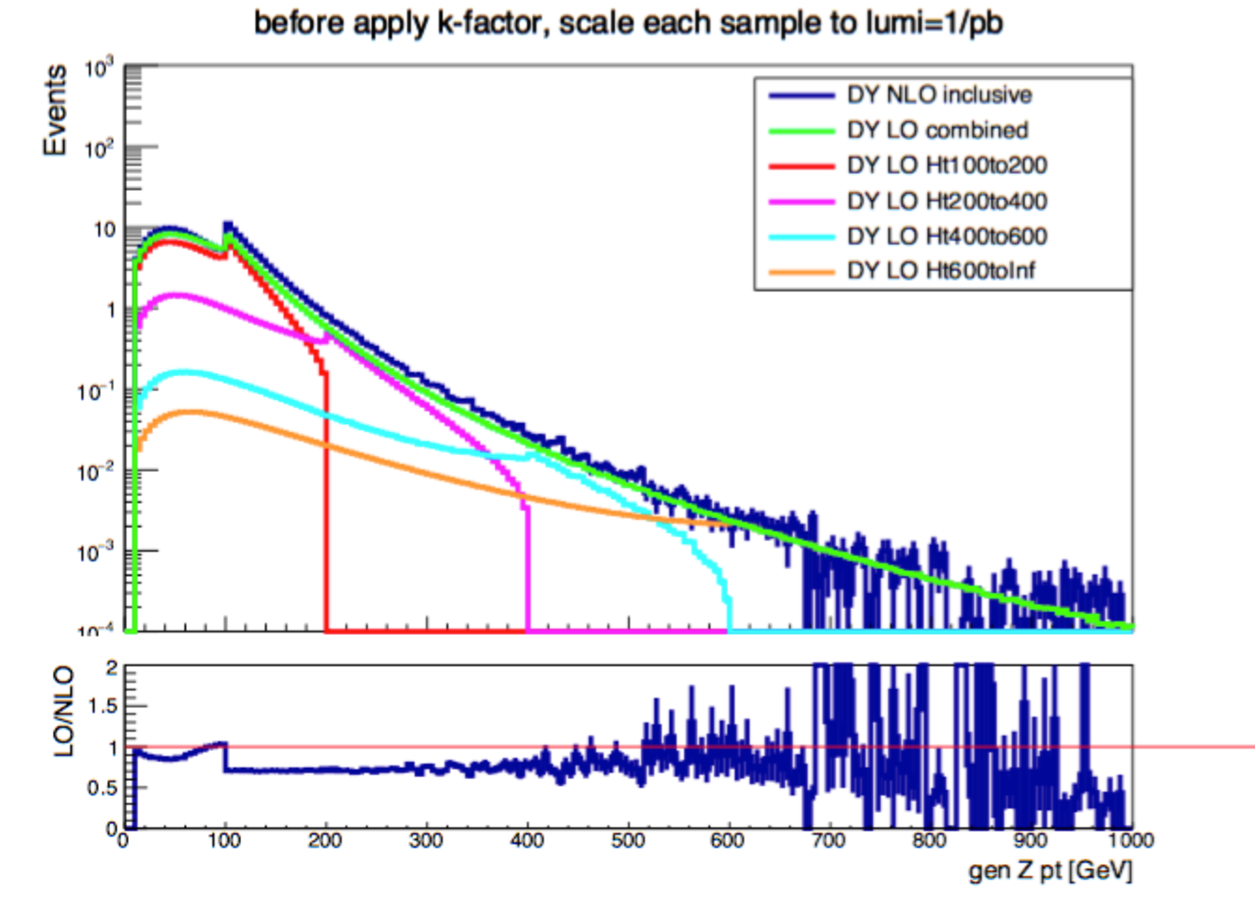
\includegraphics[width=.45\textwidth]{figures/beforeKFactorApply.pdf}\quad
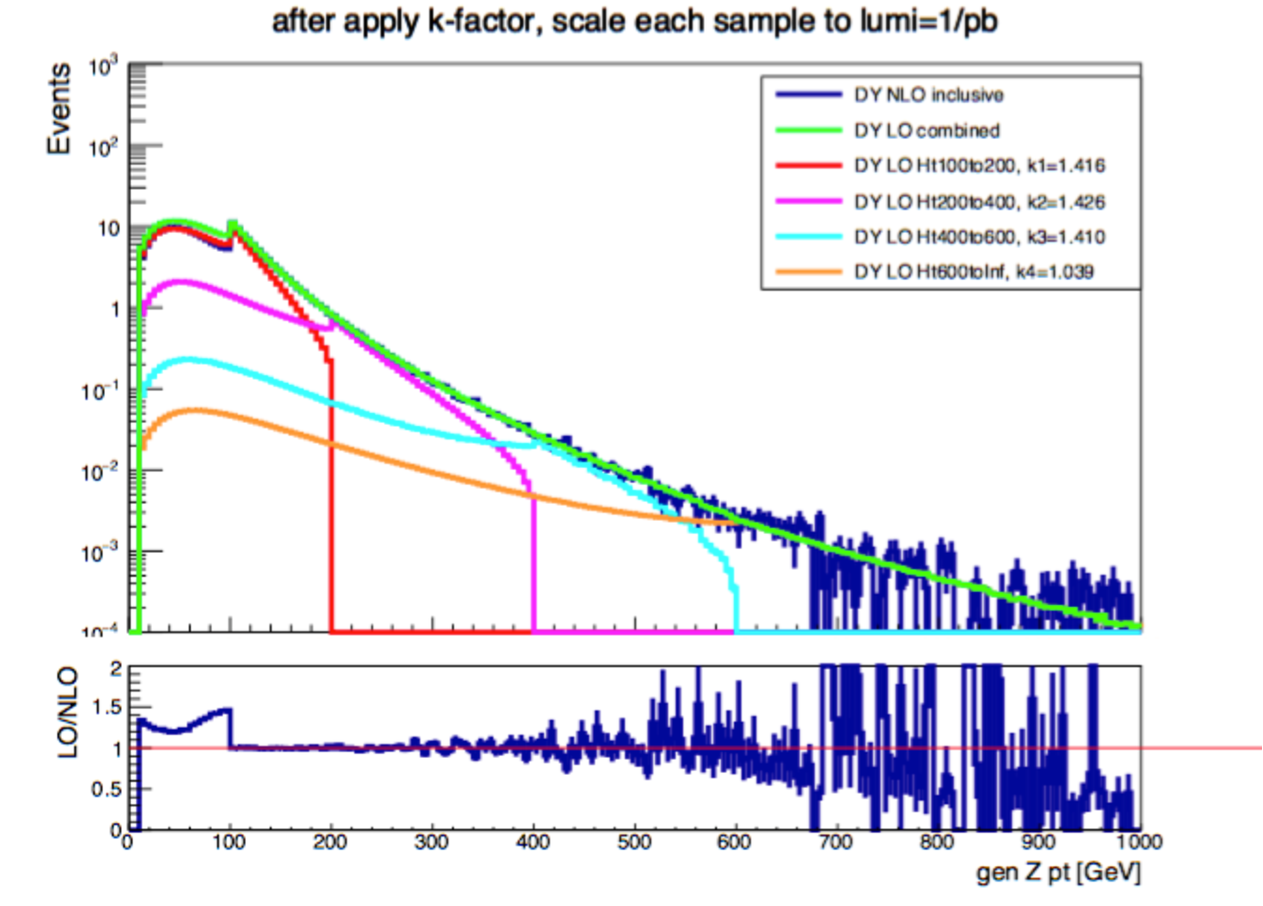
\includegraphics[width=.45\textwidth]{figures/afterKFactorApply.pdf}
\caption{The generator-level Z p$_{t}$ distributions of NLO sample, LO H$_{T}$ binned sample and the combined LO sample, before and after applying the k-factor.}
\label{pics:blablabla}
\end{figure}


\subsection{Estimating background by BumpHunting method}

Due to the insufficient statistics, we decided to use another method ``BumpHunting'' to describe the shape of background in the signal region, whereas the normalization is obtained by ALPHABET still. 

In the BumpHunting method, the background shape of the Zh invariant mass spectrum in the signal region is assumed to be similar to the shape in the sideband (passing double B-tagger and in mass window) but allow to have small bump (it's the reason for the name ``BumpHunting'') for the possibly presence of signal. Therefore, one can fit the sideband first with a function and then use the similar functional form (with initial parameters from the first fit ) to fit the signal region or do the simultaneous fit in both the sideband and the signal region. The Eqn. 5 is the fit function for the sideband, and the Eqn.6 is the same function times the averaged value of the pass/fail ratio in the signal region obtained from the ALPHABET method, which is used to describe the background in the signal region originally. But for allowing a small bump in the background shape in the signal region, one linear term ``a'' is adding to the Eqn. 6 to become Eqn.7 for the functional form used in the fit of the signal region finally.     

\begin{equation}
y=f(x) 
\end{equation}

\begin{equation}
y=R_{\frac{p}{f}}\cdot f(x) 
\end{equation}

\begin{equation}
y=(1+a\cdot x)\cdot R_{\frac{p}{f}}\cdot f(x)
\end{equation}

The fit in the sideband region is shown in Figure 9, and the function form of fit is the levelled exponential (Eqn. 8). 

\begin{equation}
y=e^{\frac{-p_{1}x}{1+p_{1}\cdot p_{2}\cdot x}}
\end{equation}

This work haven't finished and is going on still.

\begin{figure}

\centering
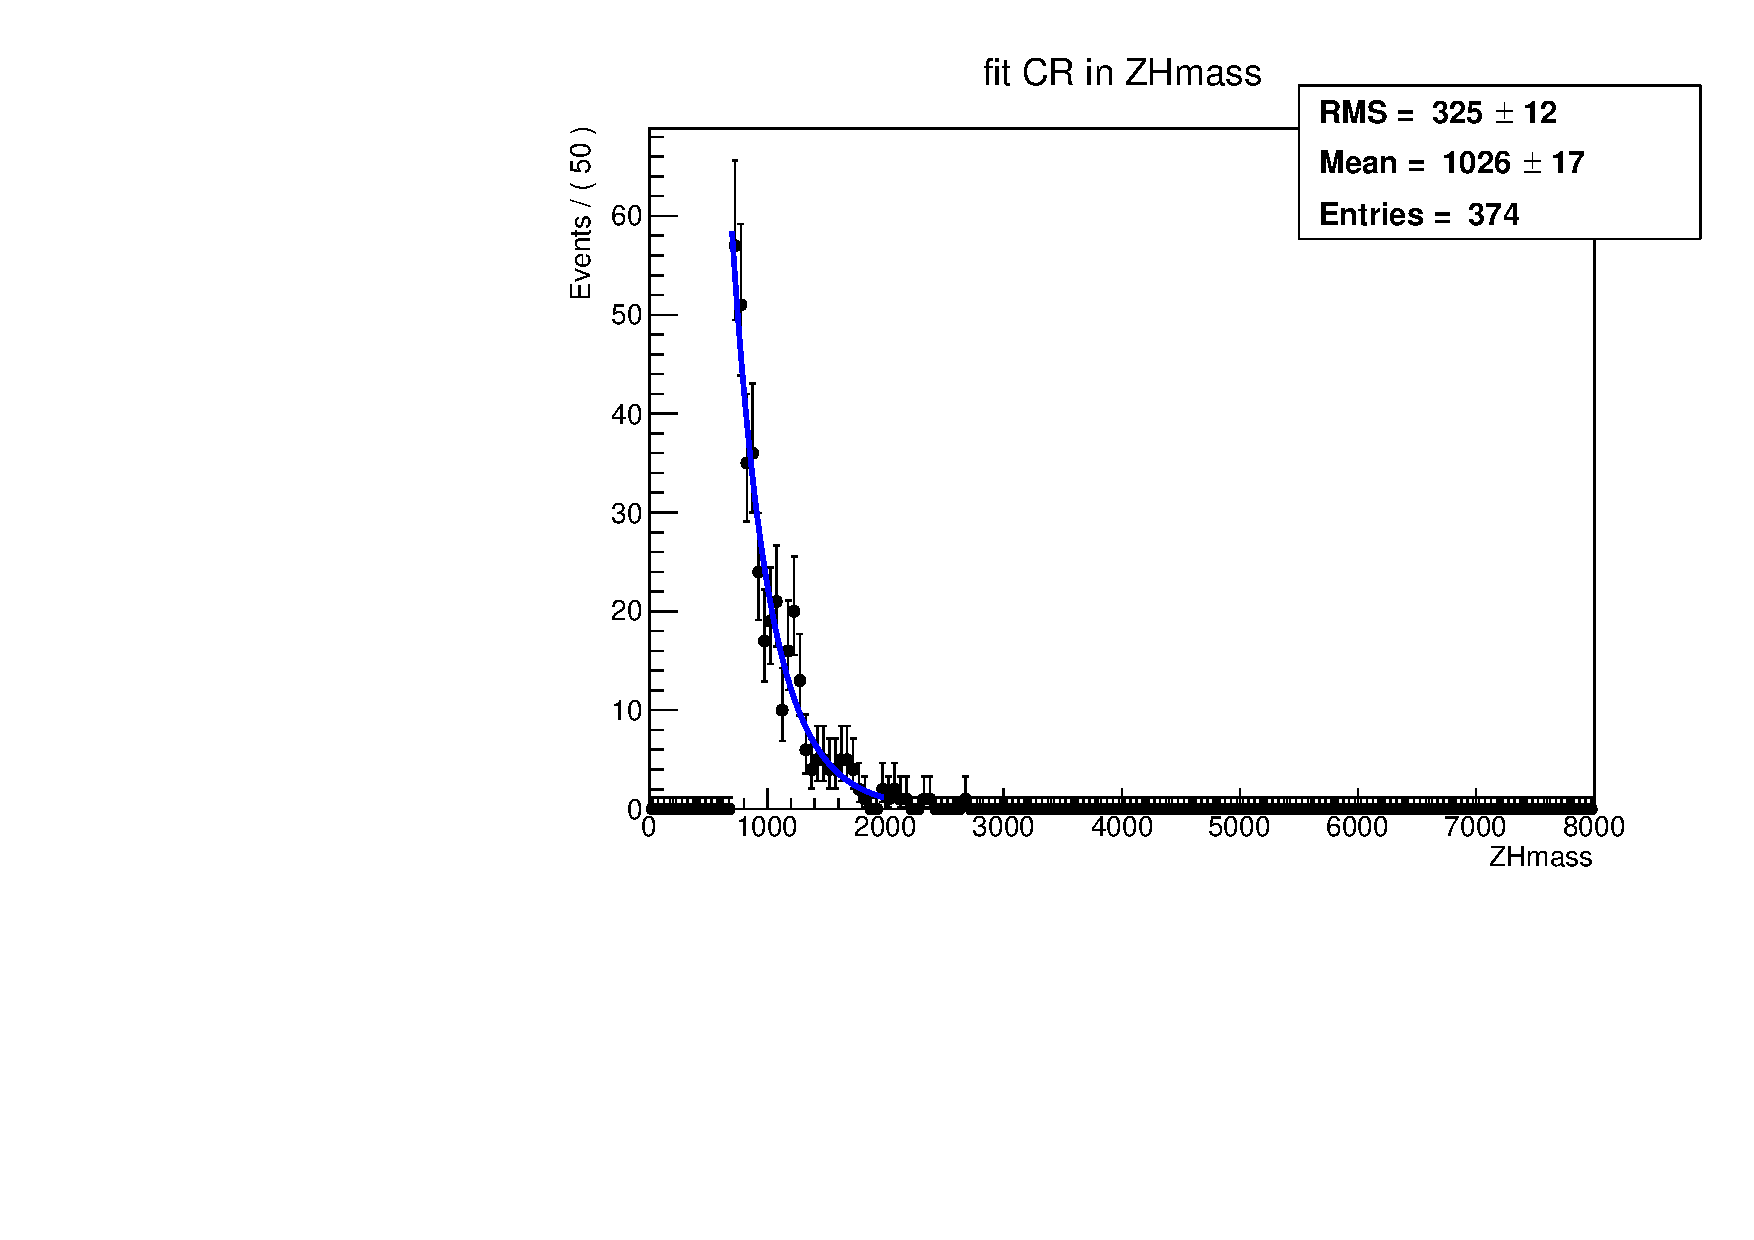
\includegraphics[width=.7\textwidth]{figures/fit_CR_in_ZHmass.pdf}
\caption{Fit the sideband, which fails the double B-tagger and is in the Soft Drop mass window, in the ZH invariant mass}
\label{pics:blablabla}
\end{figure}



\section{High Granularity Calorimeter(HGCal)}

In 2017, I continued to join the CMS phase II endcap calorimeter upgrade project ``High Granularity Calorimeter(HGCal)'' \cite{HGCal ref}. First I worked for the paper, which was the summary of our 2016 HGCal activity, then I participanted two 2017 Test Beam at CERN, May and July Test beam (mainly to take shifts). 

\subsection{2016 HGCal paper}

For the 2016 HGCal paper, which was a detector note numbered as DN-17-011 \cite{DN-17-011}, with Sandhya and Kai-Yu, who were my partners in 2016 for pedestal and noise study, we summaried our results and writed our section in paper. Beside what we already had, we added a plot of the intrinsic noise to the paper.  

For run with a lots of events on a single channel, the total noise is estimated by taking the RMS of the ADC counts distribution, and in the presence of the common mode noise, which are the noises with same amount happened in the channels of the same conditions in an events, one can define the intrinsic noise(IN noise) in Eqn9, where the ADCs$\_{i}$ is the ADC counts of i-th channels substracted the pedestal value in an event, and the N is the number of channels with the same conditions in an event. The (-1)$^{i}$ is to used to cancel the common mode noise by each pair of channels in an event, then finally the bracket is taken the RMS as the IN noise. 

\begin{equation}
\textup{IN noise}=[ \frac{\sum_{i=1}^{N}(-1)^{i}\times ADCs_{i}}{\sqrt{N}}  ]_{RMS}
\end{equation}

The intrinsic noise and the averaged total noise in different cell types are shown in Figure 10. The intrinsic noise is quite small compared to the total noise, which means the dominated noise is the common mode noise.


\begin{figure}
\centering
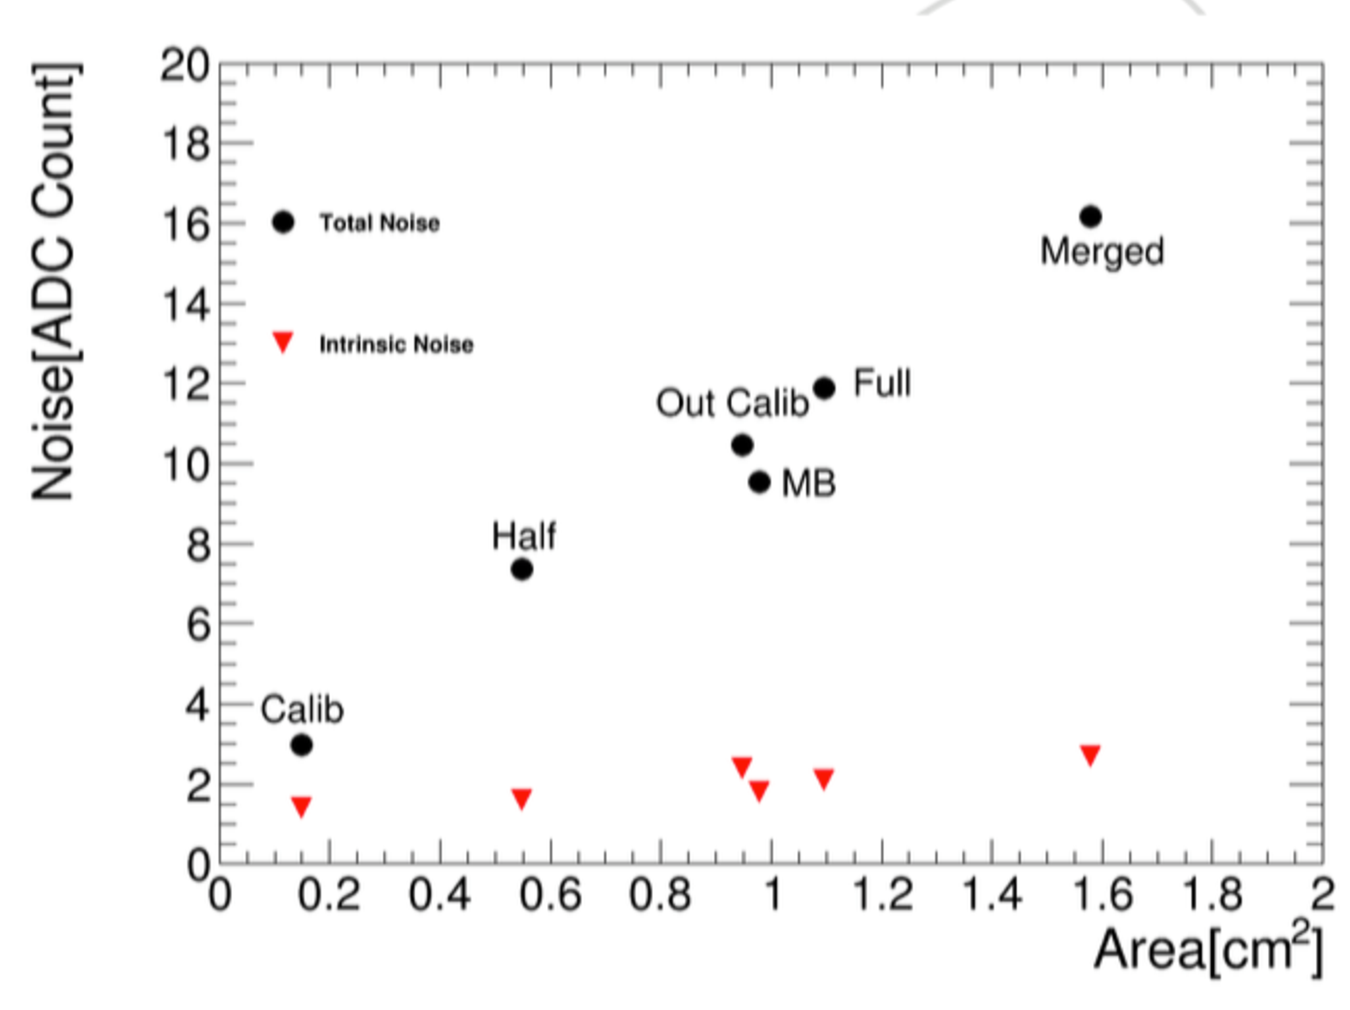
\includegraphics[width=.7\textwidth]{figures/2016Paper_Intrinsic_noise.pdf}
\caption{The averaged total noises and the intrinsic noises of different cell types}
\label{pics:blablabla}
\end{figure}



\subsection{2017 May Test Beam}

During 8$^{th}$ to 15$^{th}$ May 2017, one test beam was host in CERN's North Area beam facility (EHNA1, building 887, the H2 beamline). The purpose is to test the new ASIC chip (SKIROC-CMS, see Figure 11), new PCB, and new DAQ system (EUDAQ).

The test beam setup is shown in Figure 12. One module was tested for the EM endcap calorimeter(EE) in this test. The data of several beam energies (positron at 20,32,50,100,150,200,250 GeV \cite{May 2017 TB google doc} were taken. The electron signal could be seen as an event display shown in Figure 13. A non-showering single particle(MIP)'s signal due to the Pion contanmination was also observed as shown in Figure 14.   

\begin{figure}

\centering
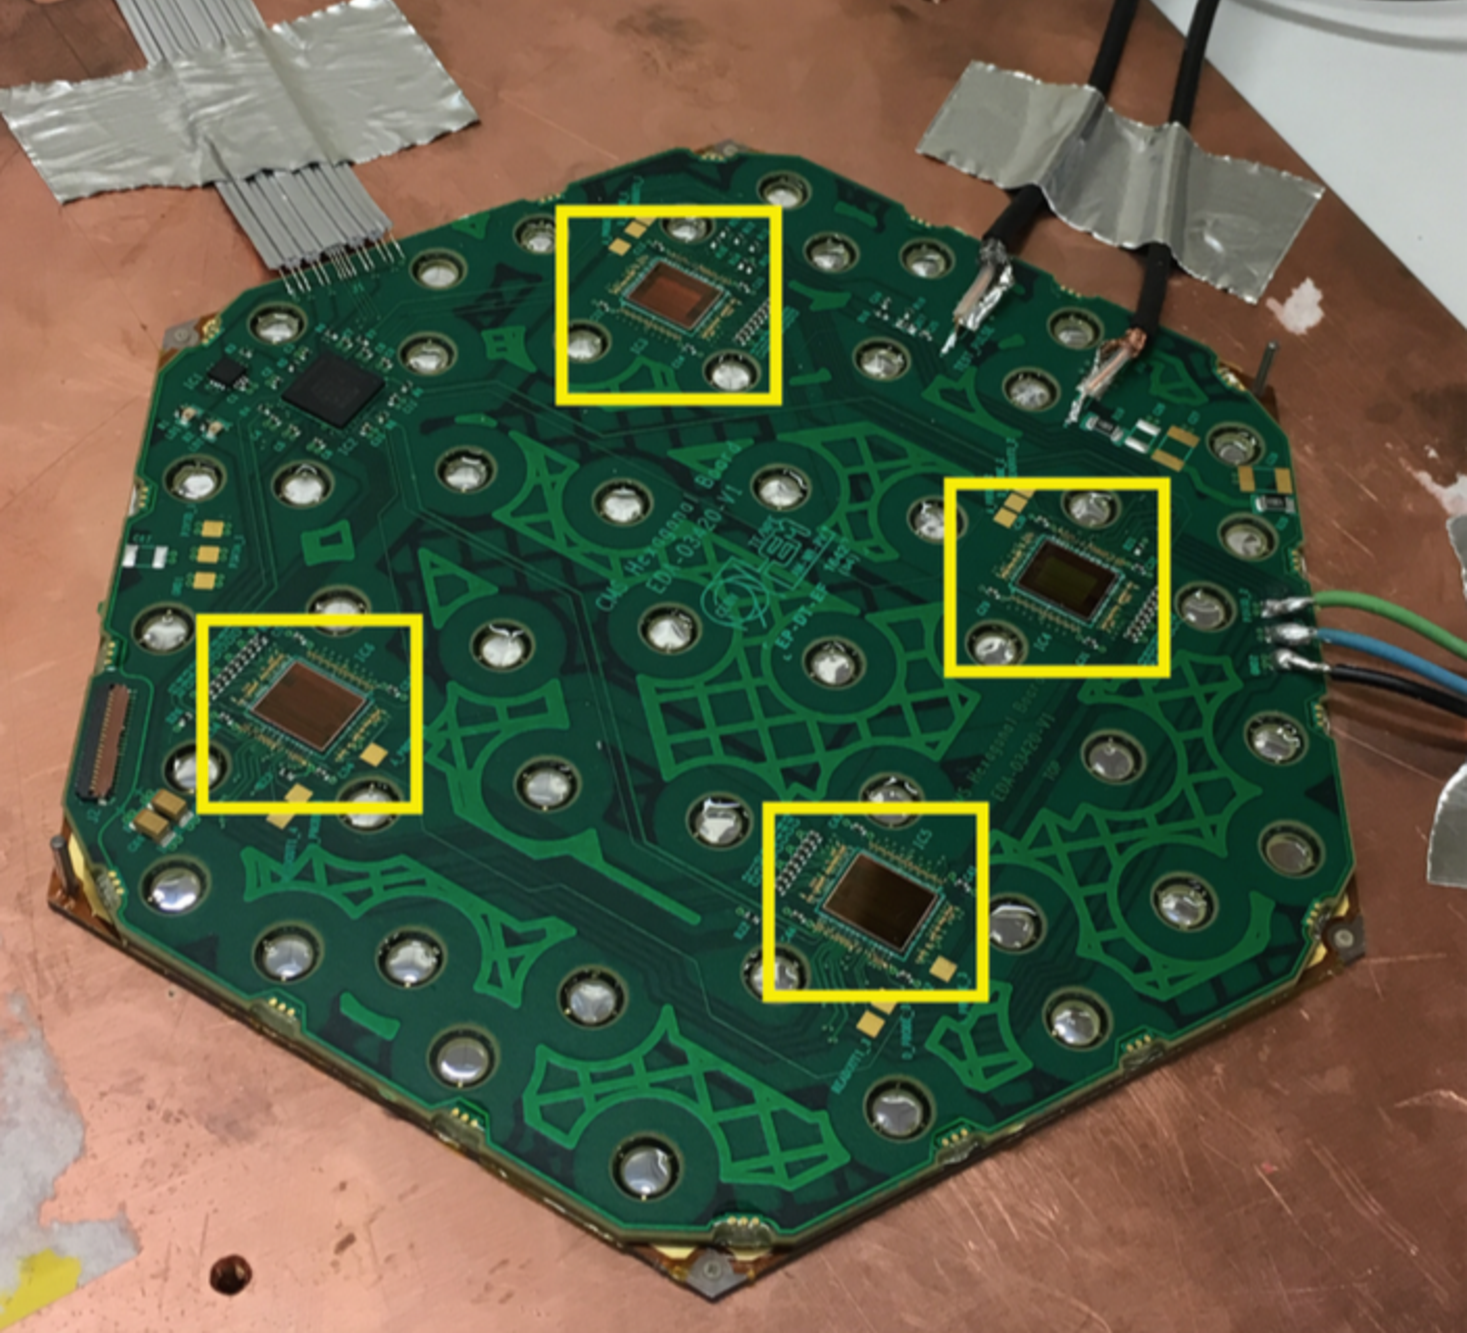
\includegraphics[width=.7\textwidth]{figures/SKIROC-CMS2_chip.pdf}

\caption{The PCB used in 2017, where 4 yellow frames indicate the SKIROC-CMS chips}
\label{pics:blablabla}
\end{figure}



\begin{figure}

\centering
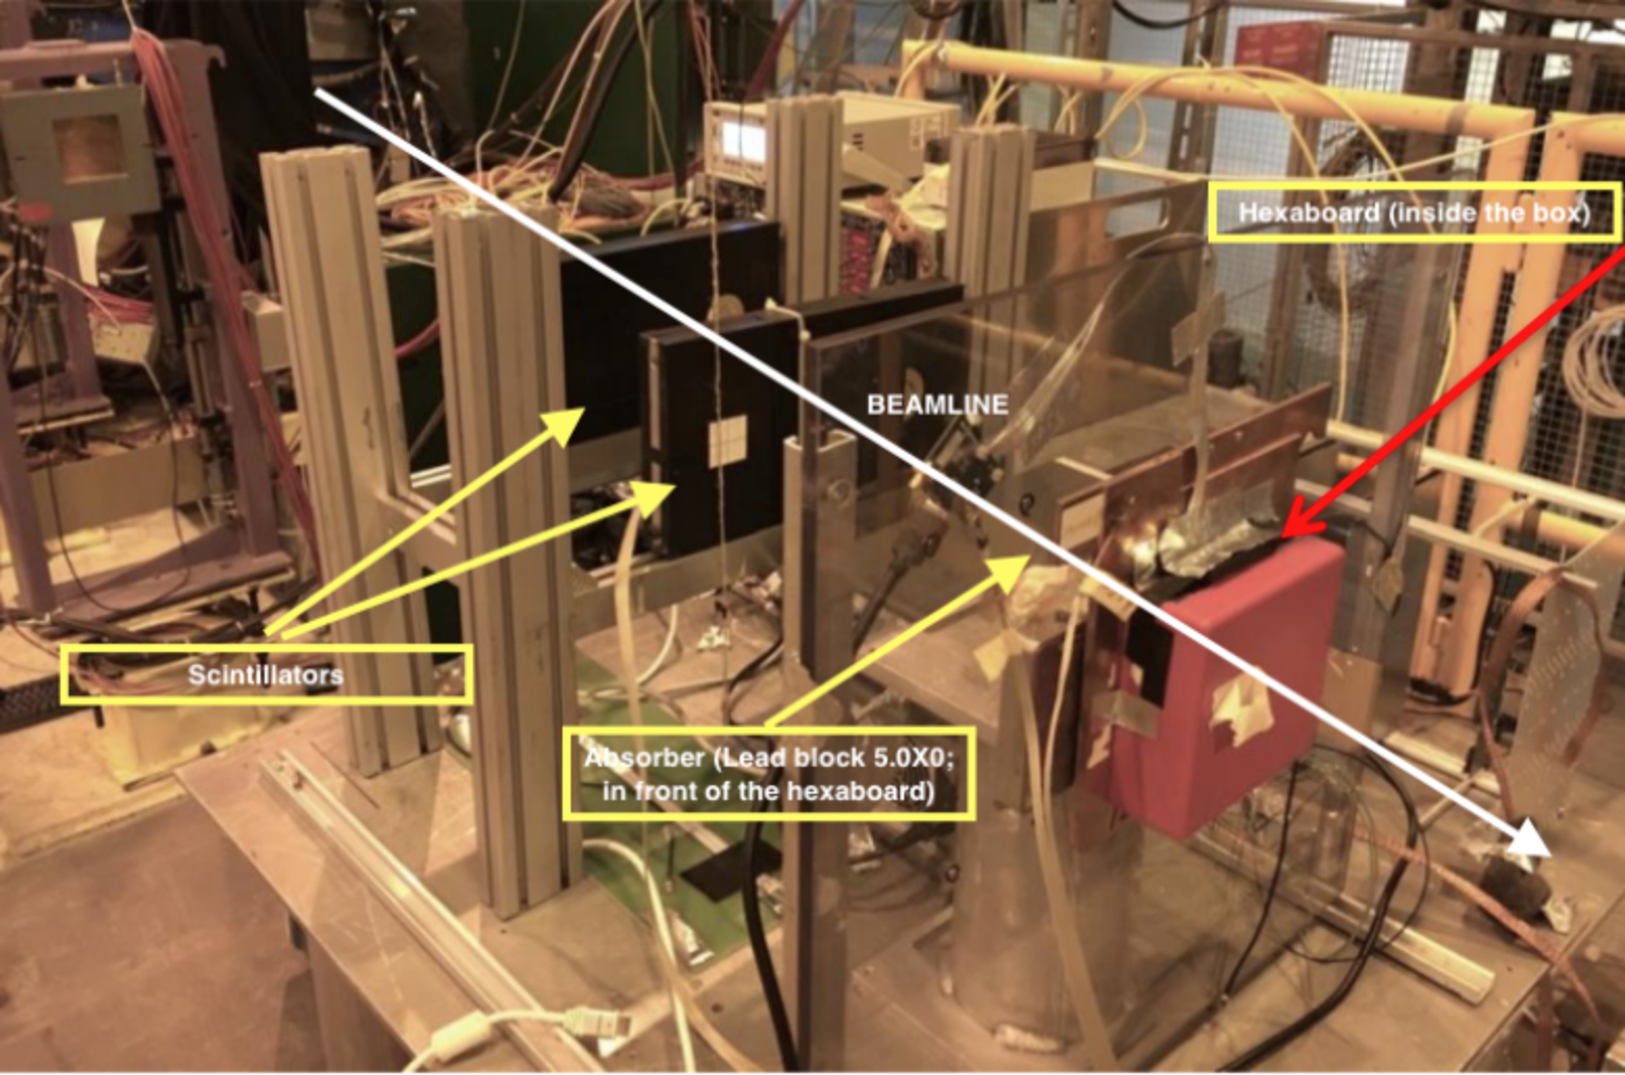
\includegraphics[width=1.\textwidth]{figures/2017MayTestBeam_Setup.pdf}

\caption{The setup of 2017 May test beam. The yellow framed texts indicate the scintillators, absorber and the hexaboard (module containing the Silicon sensor,PCB ...etc). The beam direction is indicated by a white arrow.}
\label{pics:blablabla}
\end{figure}




\begin{figure}

\centering
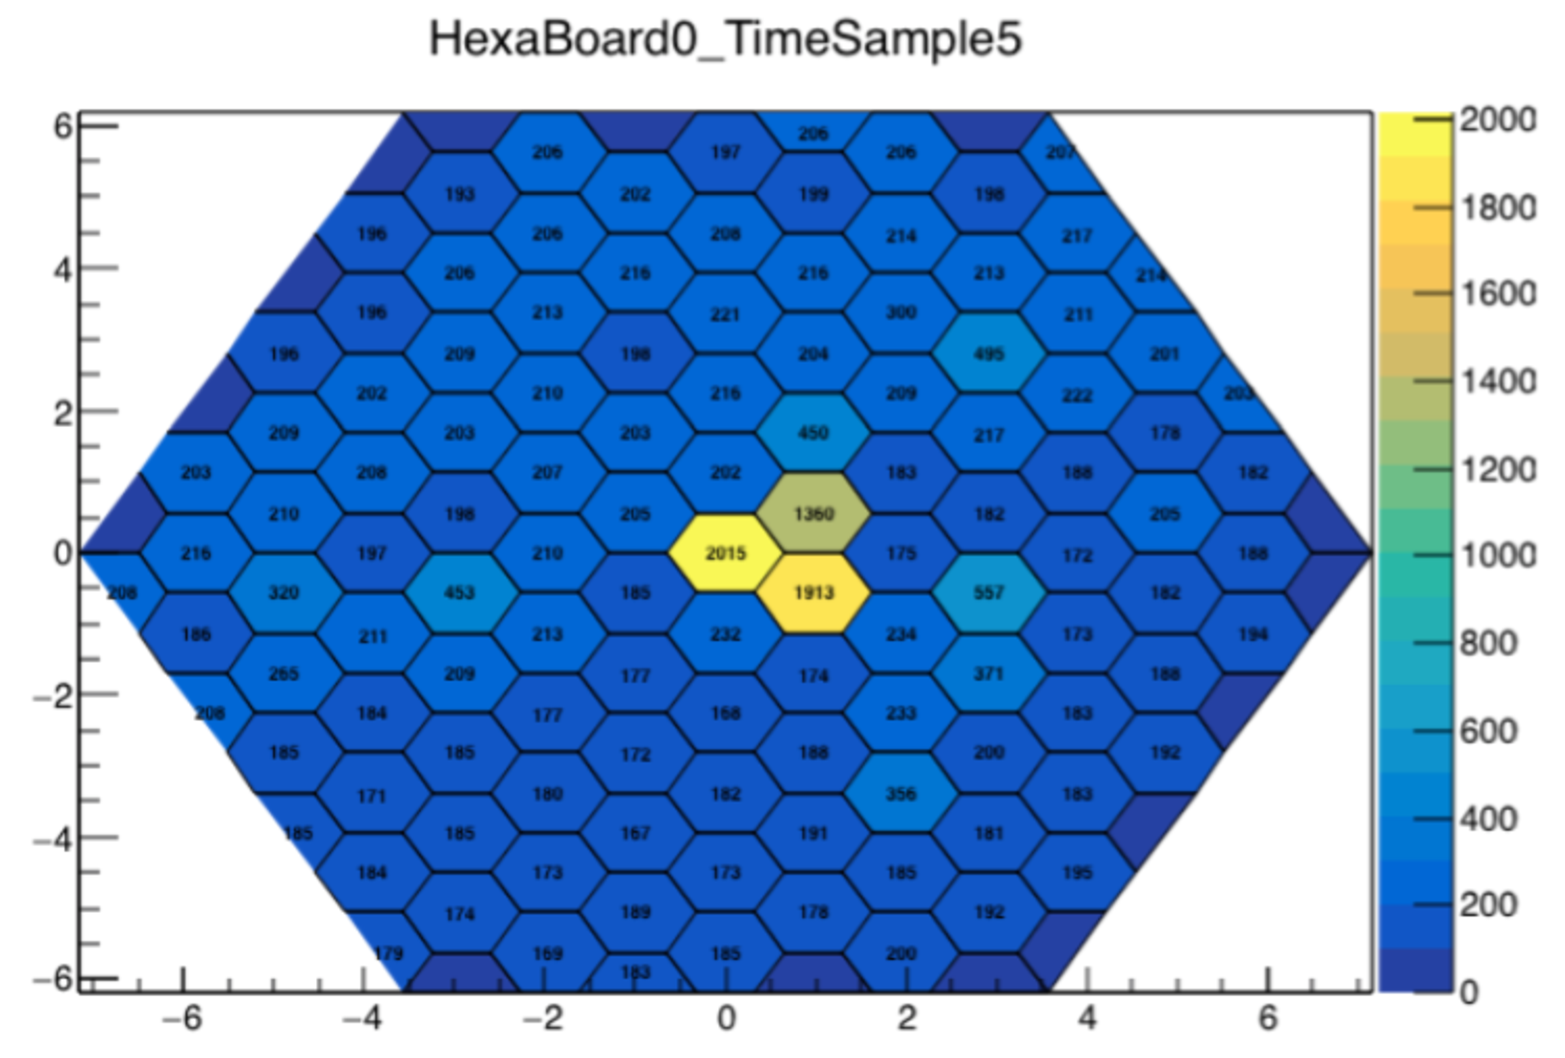
\includegraphics[width=1.\textwidth]{figures/2017MayTestBeam_eventDisplay1.pdf}

\caption{An event display of run 106 (positron beam at 150 GeV), event 64, time sample 5}
\label{pics:blablabla}
\end{figure}


\begin{figure}
\centering
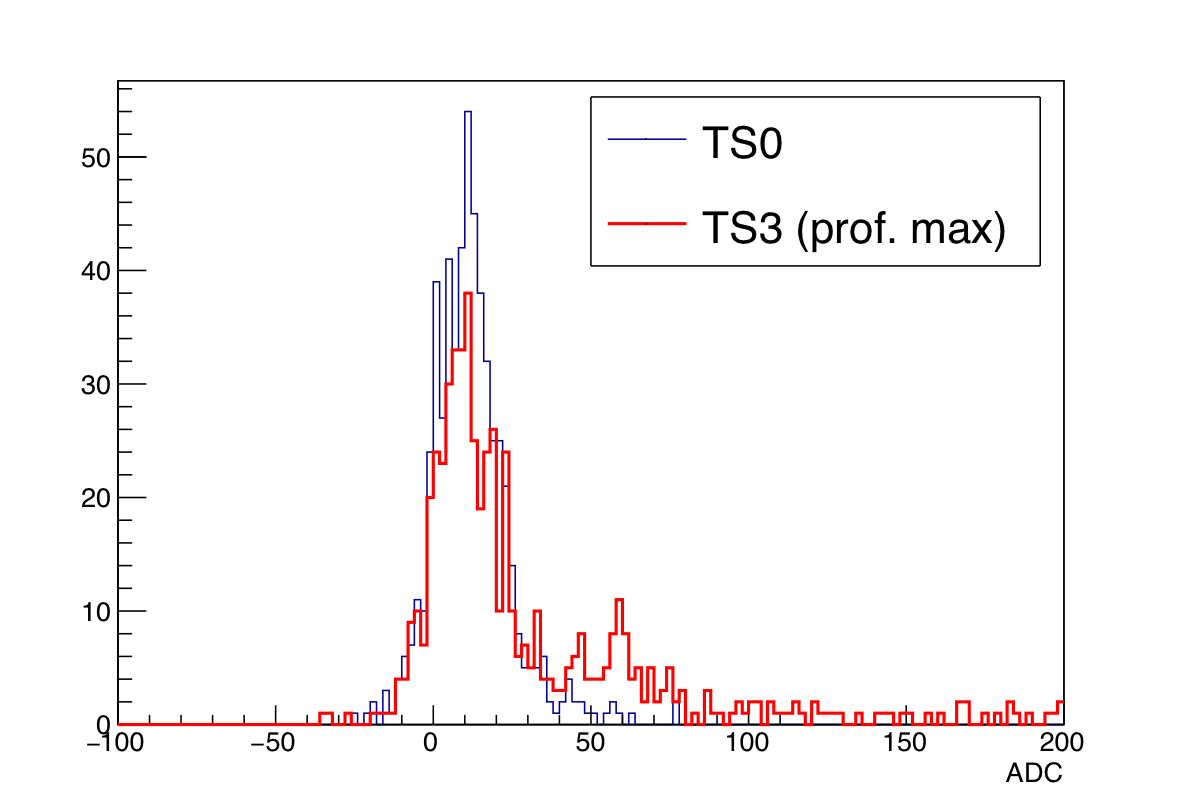
\includegraphics[width=1.\textwidth]{figures/MIP_ch1_36_ref_ch1_58.png}
\caption{High gain ADCs distribution of chip=1/channel=36(from the center of hexaboard where beam hits)/SCA=0/time sample=0 or 3. The good run 111-122 (around 11000 events) with electron beam at 200 GeV was used. The pion contamination could have possibility to cause MIP in time sample 3, and the time sample 0 shown the noise-like behavior by contrast. To reduce the significant common mode noise, chip=1/channel=58(from position not hit by beam)/SCA=0/time sample=0 or 3 had been used as the reference (to be subtracted). A peak was clearly visible around 60 ADC for the MIP.} 
\label{pics:blablabla}
\end{figure}


One feature of May test beam (and July test beam) in 2017 is the ASIC chip ``SKIROC-CMS'' can save thirdteen time samples, whereas the ASIC chip used in 2016 saved one time sample only, so this provides us more information to analyze the data (but also more complicated). 

In each channel of the SKIROC-CMS chip there are 13 switched capacitor array(SCA) to save the charges received from the Silicon sensor in turns of the period of 25 ns per SCA. Once the 13-th SCA has been charged the amount in that 25 ns period, then the first SCA will be discharged (erase original information) and charged again for the next 25 ns period. This cycle will keep going until the trigger signal arrives, whose delay time is around 200 ns (if \textgreater 25x13 ns then we lost the event), then the whole 13 SCAs' information (the amount of charges) will be send out, and in this step the 13 SCAs will be called 13 time samples according to the coming order, where the two SCAs near the trigger become the 12th and 13th time samples as the cartoon shown in Figure 15.    

Except the last 4 time samples' values, which do not reflect the charges received in the Silicon sensor due to the tigger signal, the values of other 9 time samples describ the pulse shape in an event as in Figure 16.    

In the pedestal run in May test beam ( and aslo in July test beam), there are few good runs and a lot of bad run as the examples shown in Figure 17 and Figure 18. Since it's hard to find a stable pedestal run to represent the pedestal in all times, finally we decided to use the first SCA as the pedestal value to do the pedestal subtraction in every event.  


\begin{figure}
\centering
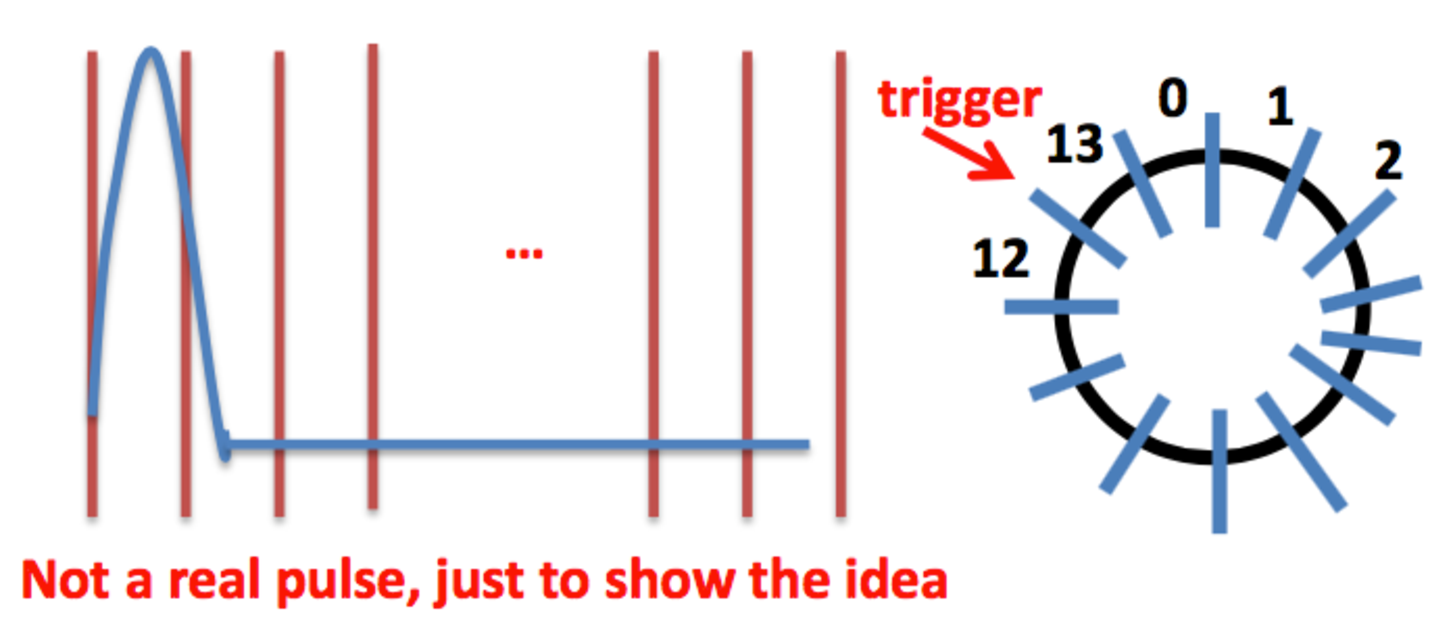
\includegraphics[width=.7\textwidth]{figures/SCA_and_TimeSample2.pdf}
\caption{A cartoon shows how the capacitors sample the pulse shape, which is the charges received Silicon sensor in different time(left) and the relationship of SCA and the time sample.}
\label{pics:blablabla}
\end{figure}

\begin{figure}
\centering
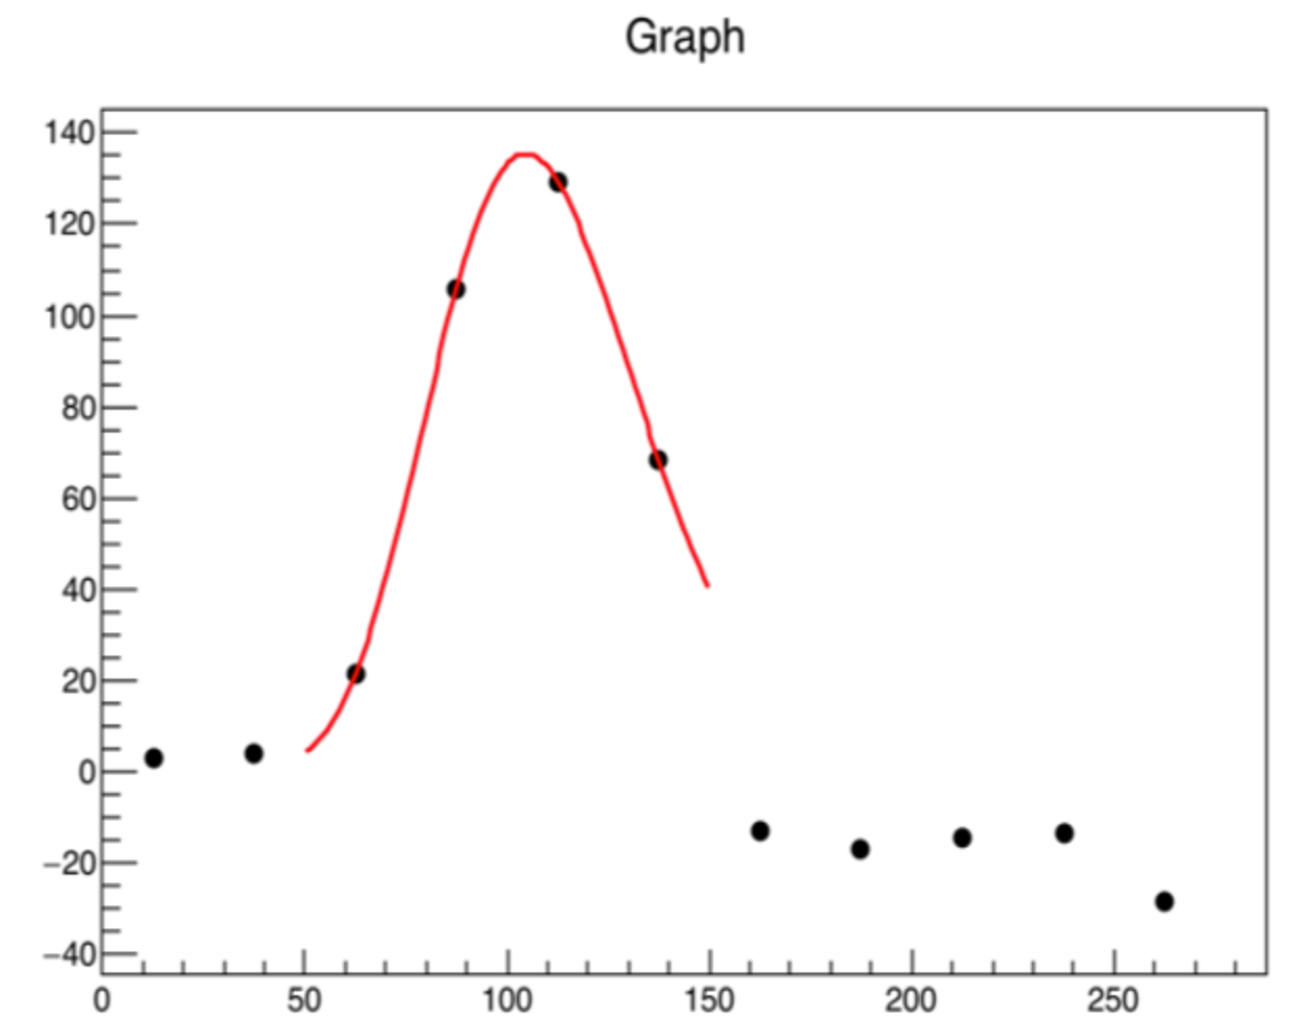
\includegraphics[width=.7\textwidth]{figures/Shilpi_fit_TimeSample_shape.pdf}
\caption{Among 9 time samples of an event, using time sample 3,4,5,6 to fit and find the time of arrival and the time of maximun}
\label{pics:blablabla}
\end{figure}


\begin{figure}
\centering
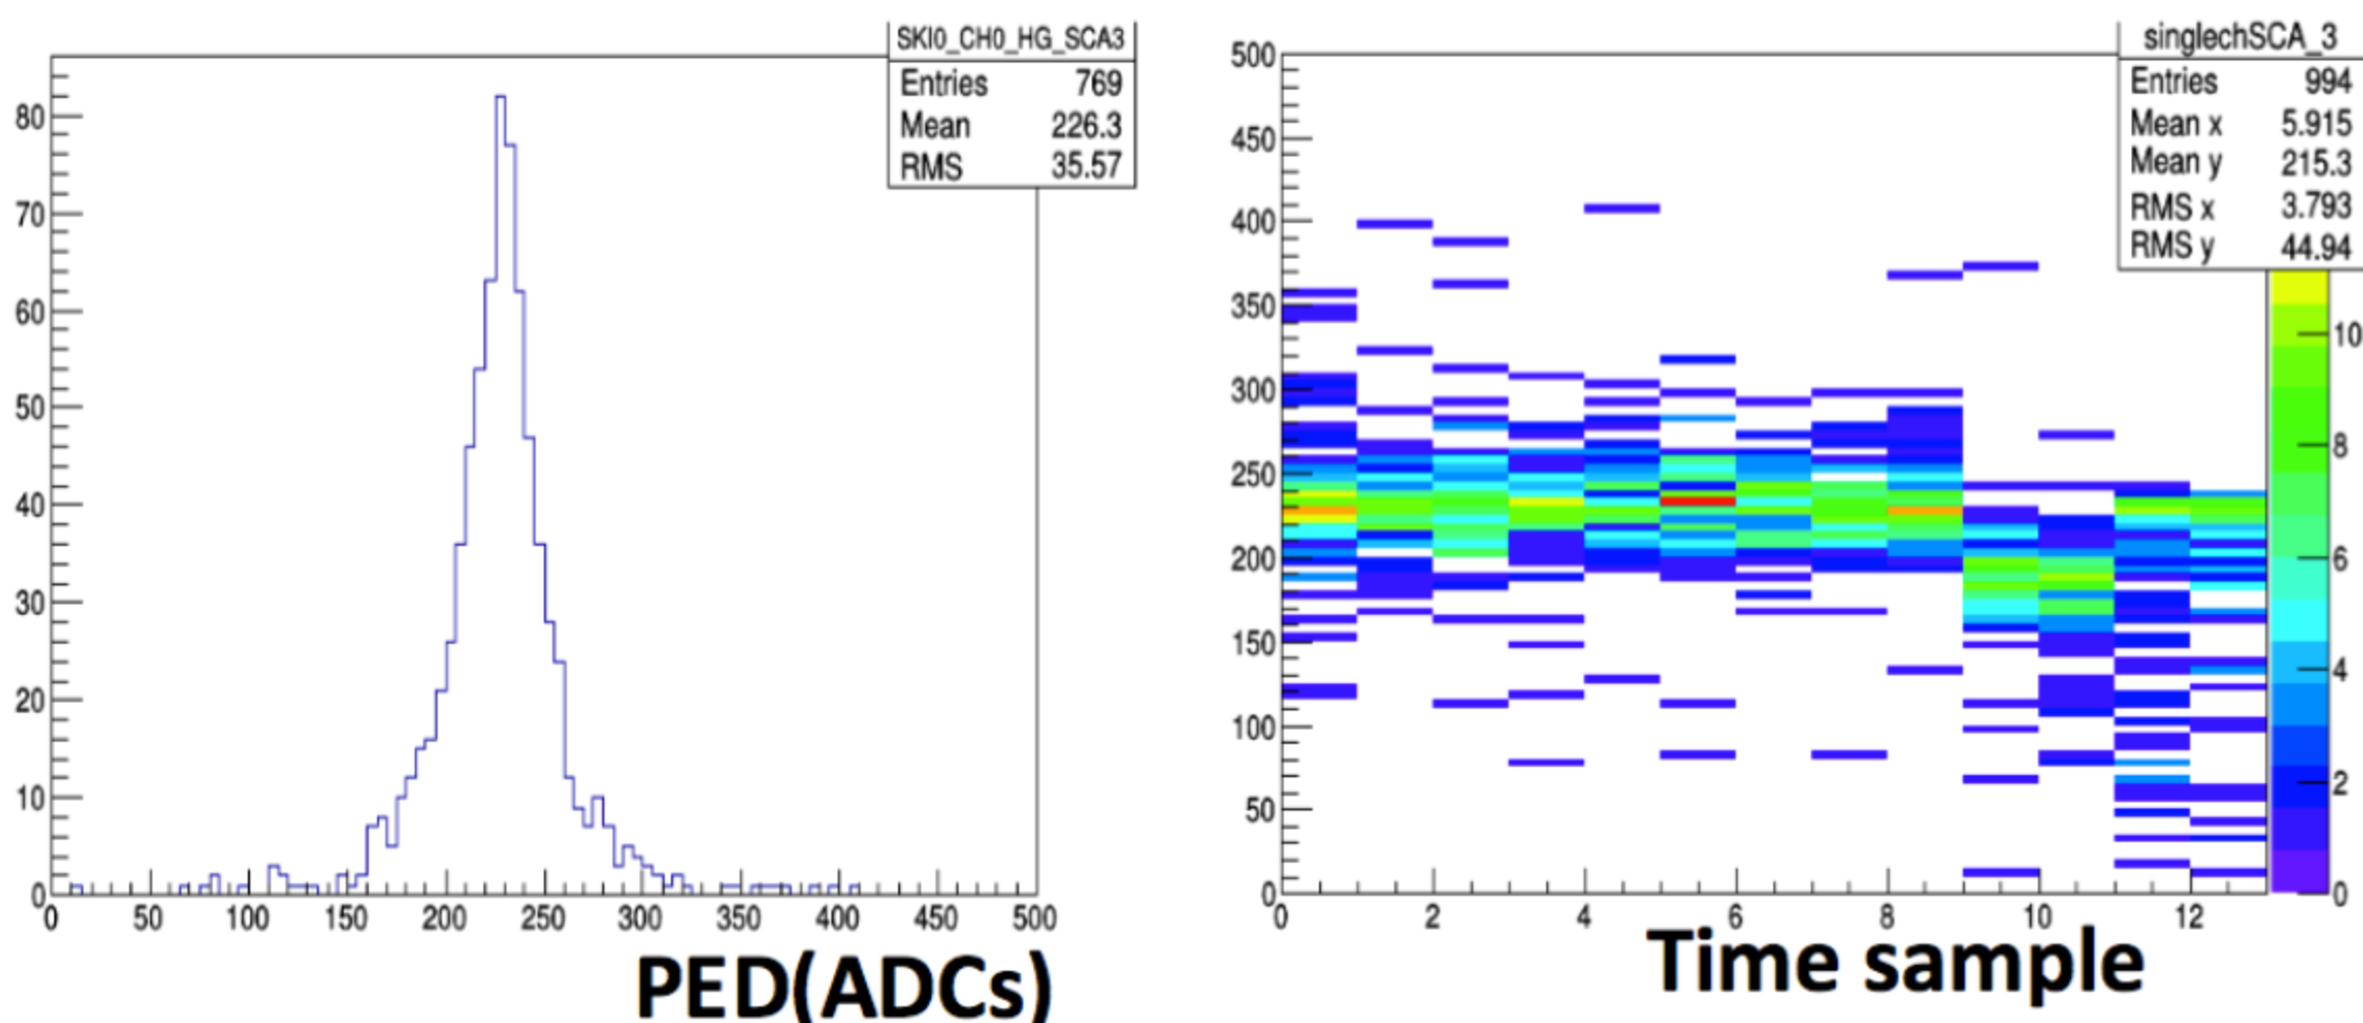
\includegraphics[width=.7\textwidth]{figures/goodPEDrun.pdf}
\caption{ADCs distribution in histogramof all time sample (left) and profile of time sample (right) of a good run 93  }
\label{pics:blablabla}
\end{figure}


\begin{figure}
\centering
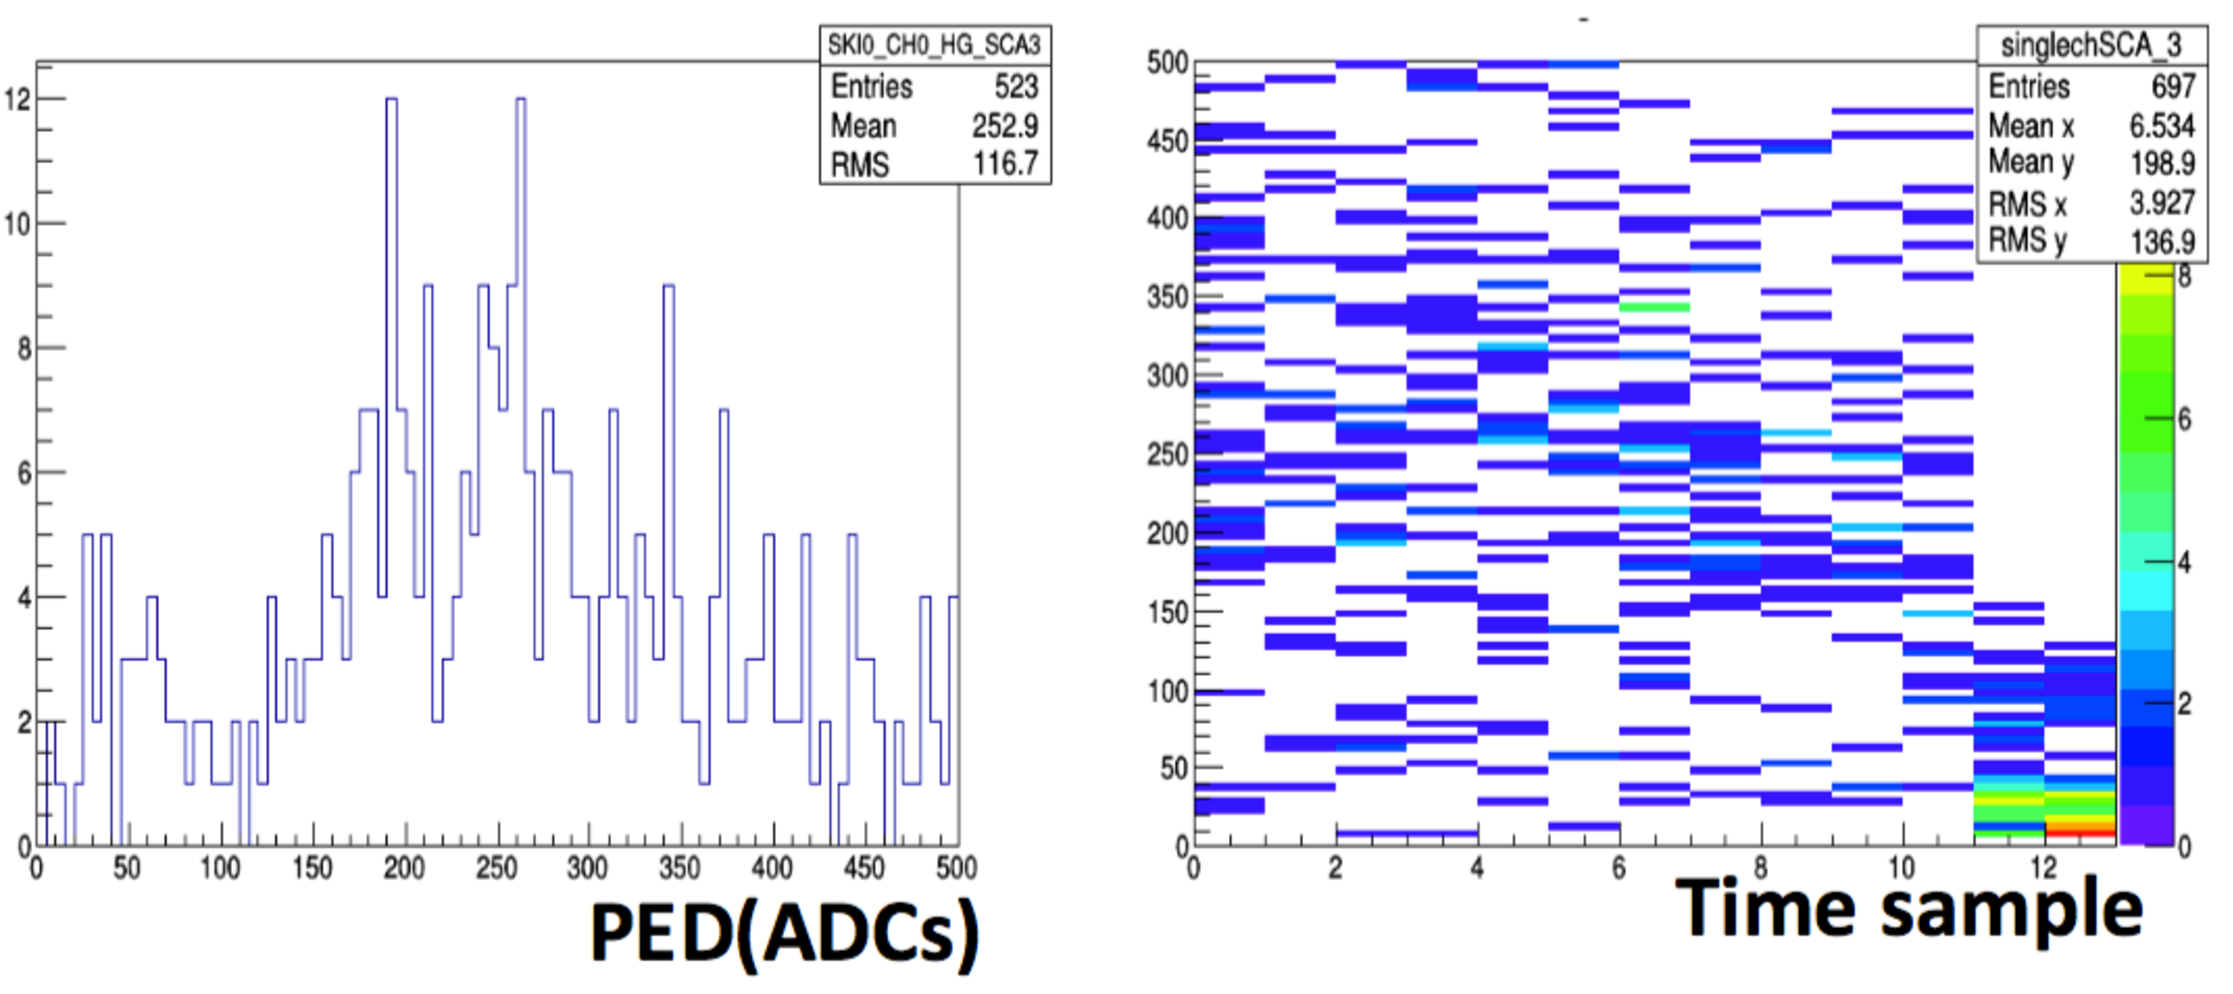
\includegraphics[width=.7\textwidth]{figures/badPEDrun.pdf}
\caption{ADCs distribution in histogramof all time sample (left) and profile of time sample (right) of a bad run 53 }
\label{pics:blablabla}
\end{figure}



\subsection{2017 July Test Beam}

During 12$^{th}$ to 19$^{th}$ July 2017, another test beam was host in the same place. The purpose is to measure the hadronic shower in the front hadron calorimeter(FH). Due to the nuclear interaction length (the mean free path of a nuclear interacting particle) is usually larger than the radiation length, the width of hadronic shower is also larger than the width of EM shower, therefore we bound three modules (instead of one in May) together in the Copper cooling plate to cover the wide width of the hadronic shower (see Figure 15). However, the limited number of modules in hands in that time forced us to use one module per layer for two layers (1+1) to mimic the EE part and use one module per layer for two layers and three modules per layer for two layers (1+1+3+3) to mimic the FH part. In the downstream of FH, we borrowed the AHCAL modules from the CALICE experiment \cite{CALICE ref} to mimic the backing hadron calorimeter(BH). The setup of full July test beam and the side view of FH are shown in Figure 16 and Figure 17. 

In the period of data-taking, we had ever difficult time for the low data-taking rate (this was solved after the IPbus protocol between the chip and EUDAQ PC was established) and the EUDAQ stuck, so only in the last 8 hours after we fixed all issues we could take more statistical data. The data of pion beam (at 100, 150, 200, 250 and 300 GeV), electon beam(at 150 and 250 GeV), and muon beam (at 150 GeV)are taken \cite{July 2017 TB google doc}. One event display of HCal and the monitoring of AHCAL data-taking are shown in Figure 18 and Figure 19.   

After the booking period, we also kept our setup in H2 beamline and benifited from the experiments in the upstream of us in either using the residue muons or that they allow us to use the beam in their spare time to take more data.  


\begin{figure}
\centering
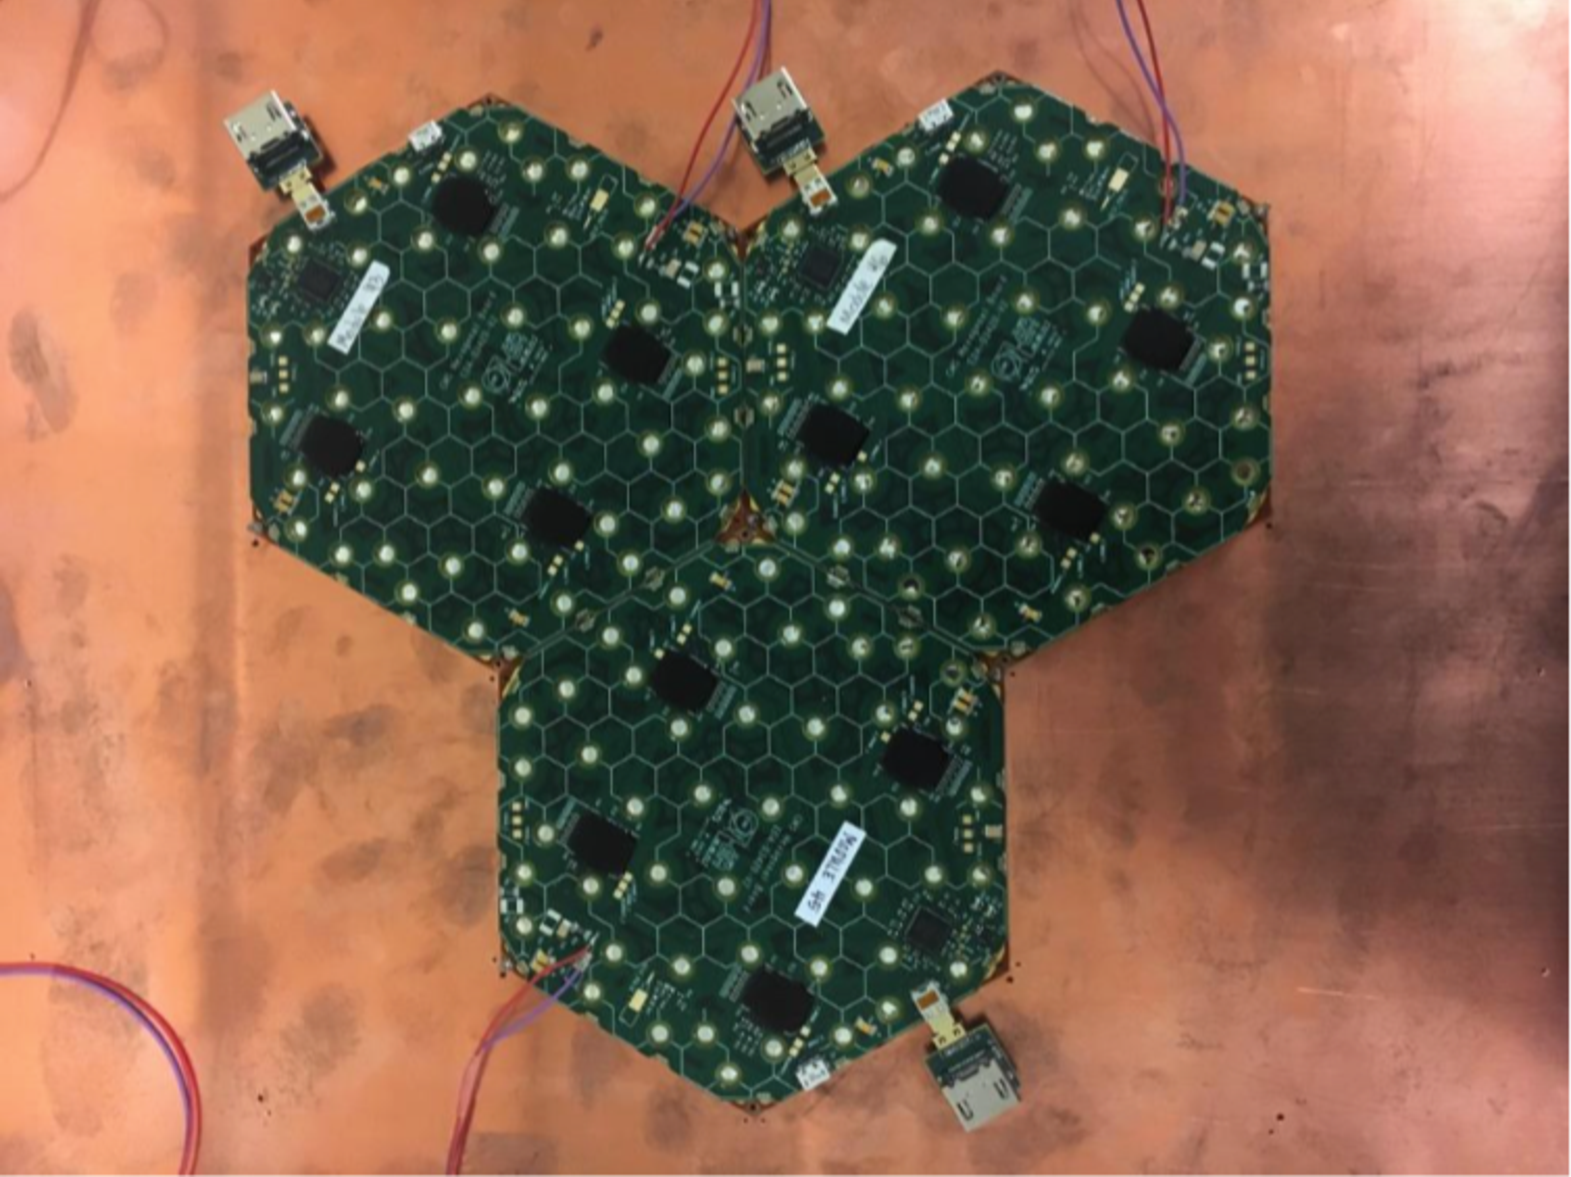
\includegraphics[width=.7\textwidth]{figures/2017JulyTestBeam_3moduleForFH.pdf}
\caption{Three modules glued in one copper cooling plate}
\label{pics:blablabla}
\end{figure}

\begin{figure}
\centering
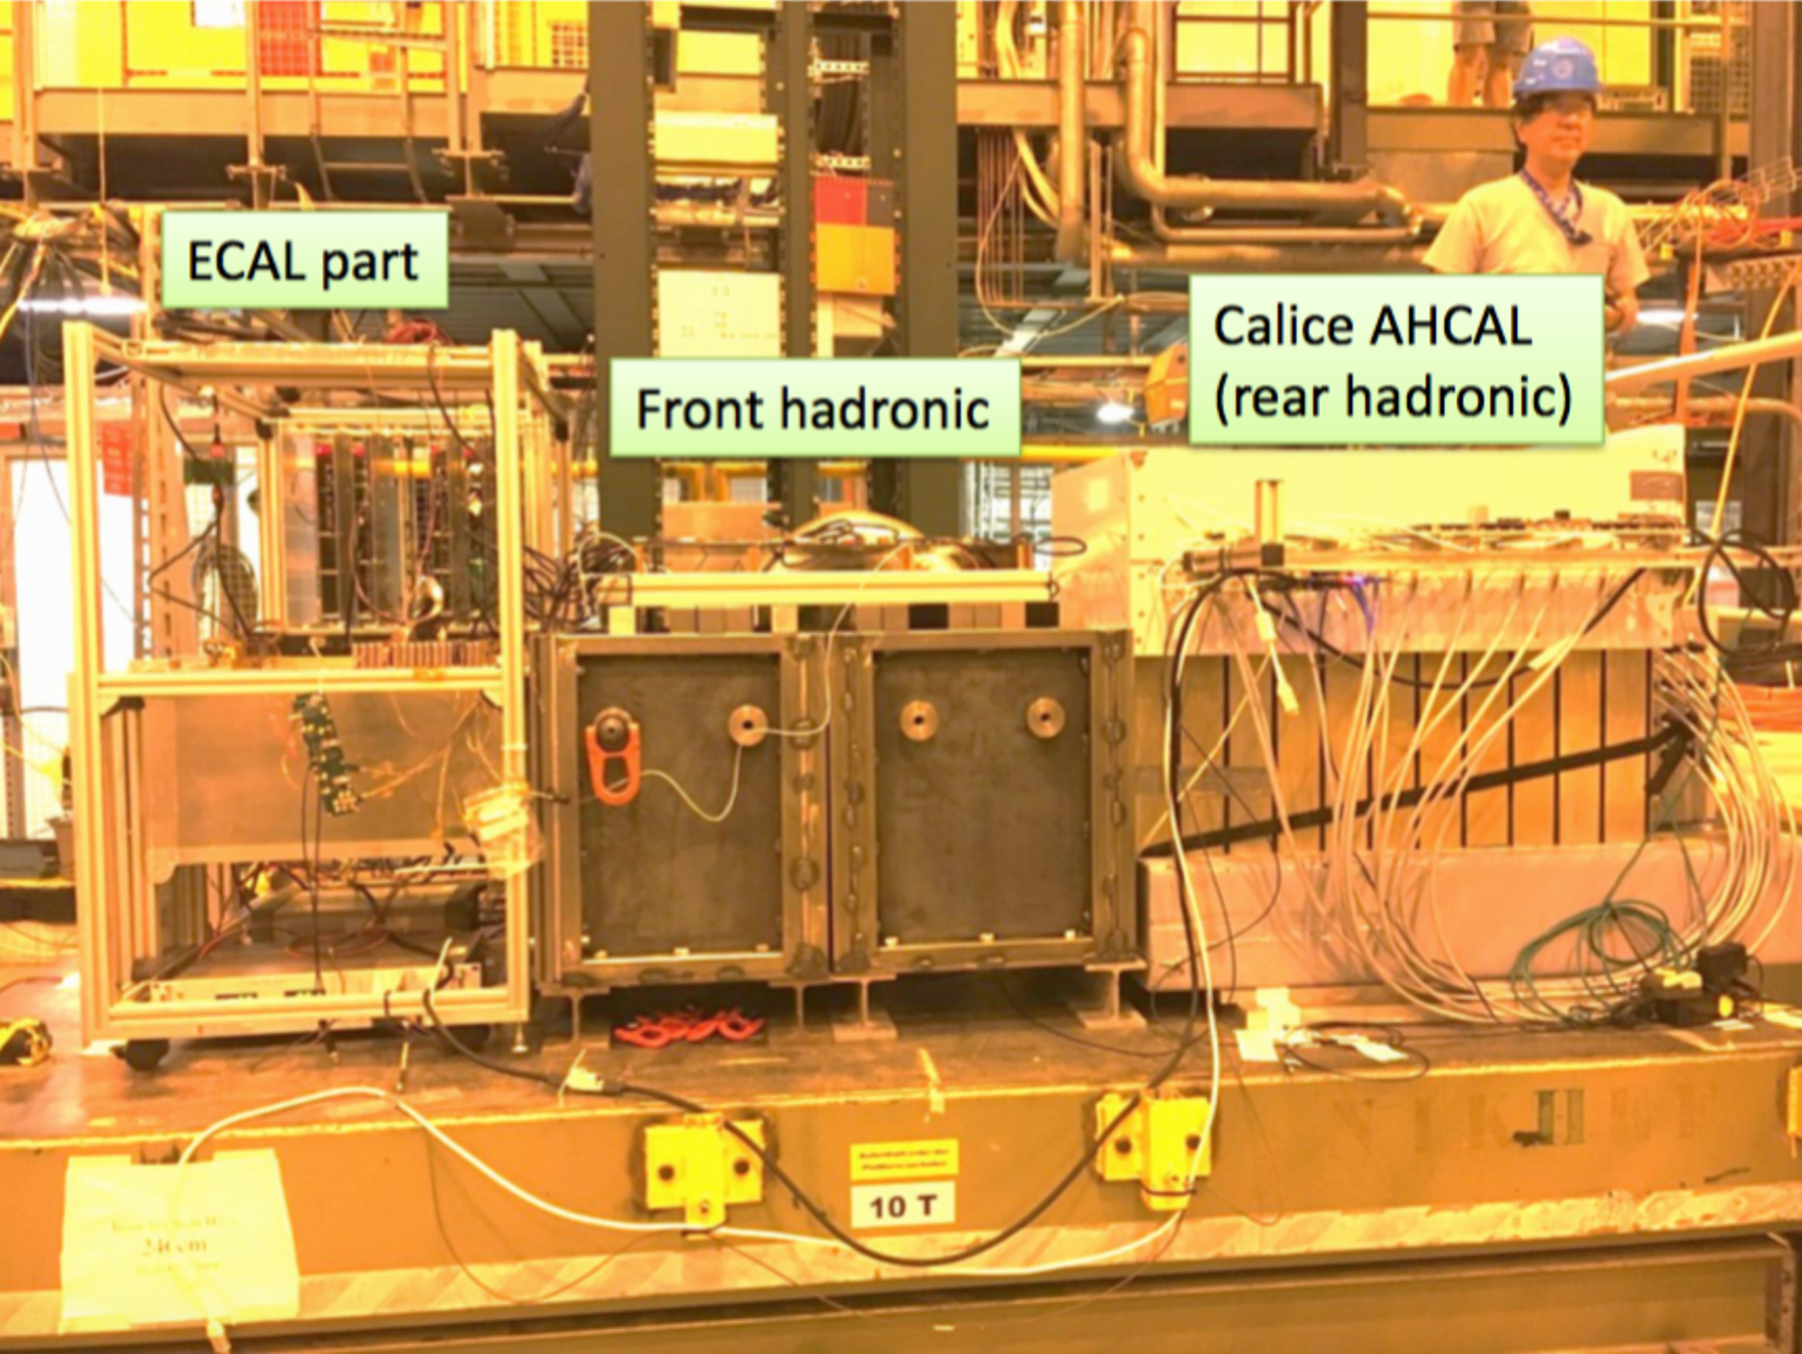
\includegraphics[width=.7\textwidth]{figures/2017JulyTestBeam_setup1.pdf}
\caption{The setup of 2017 May test beam, which contain the ECAL and FH and AHCAL from left to right (beam direction)}
\label{pics:blablabla}
\end{figure}

\begin{figure}
\centering
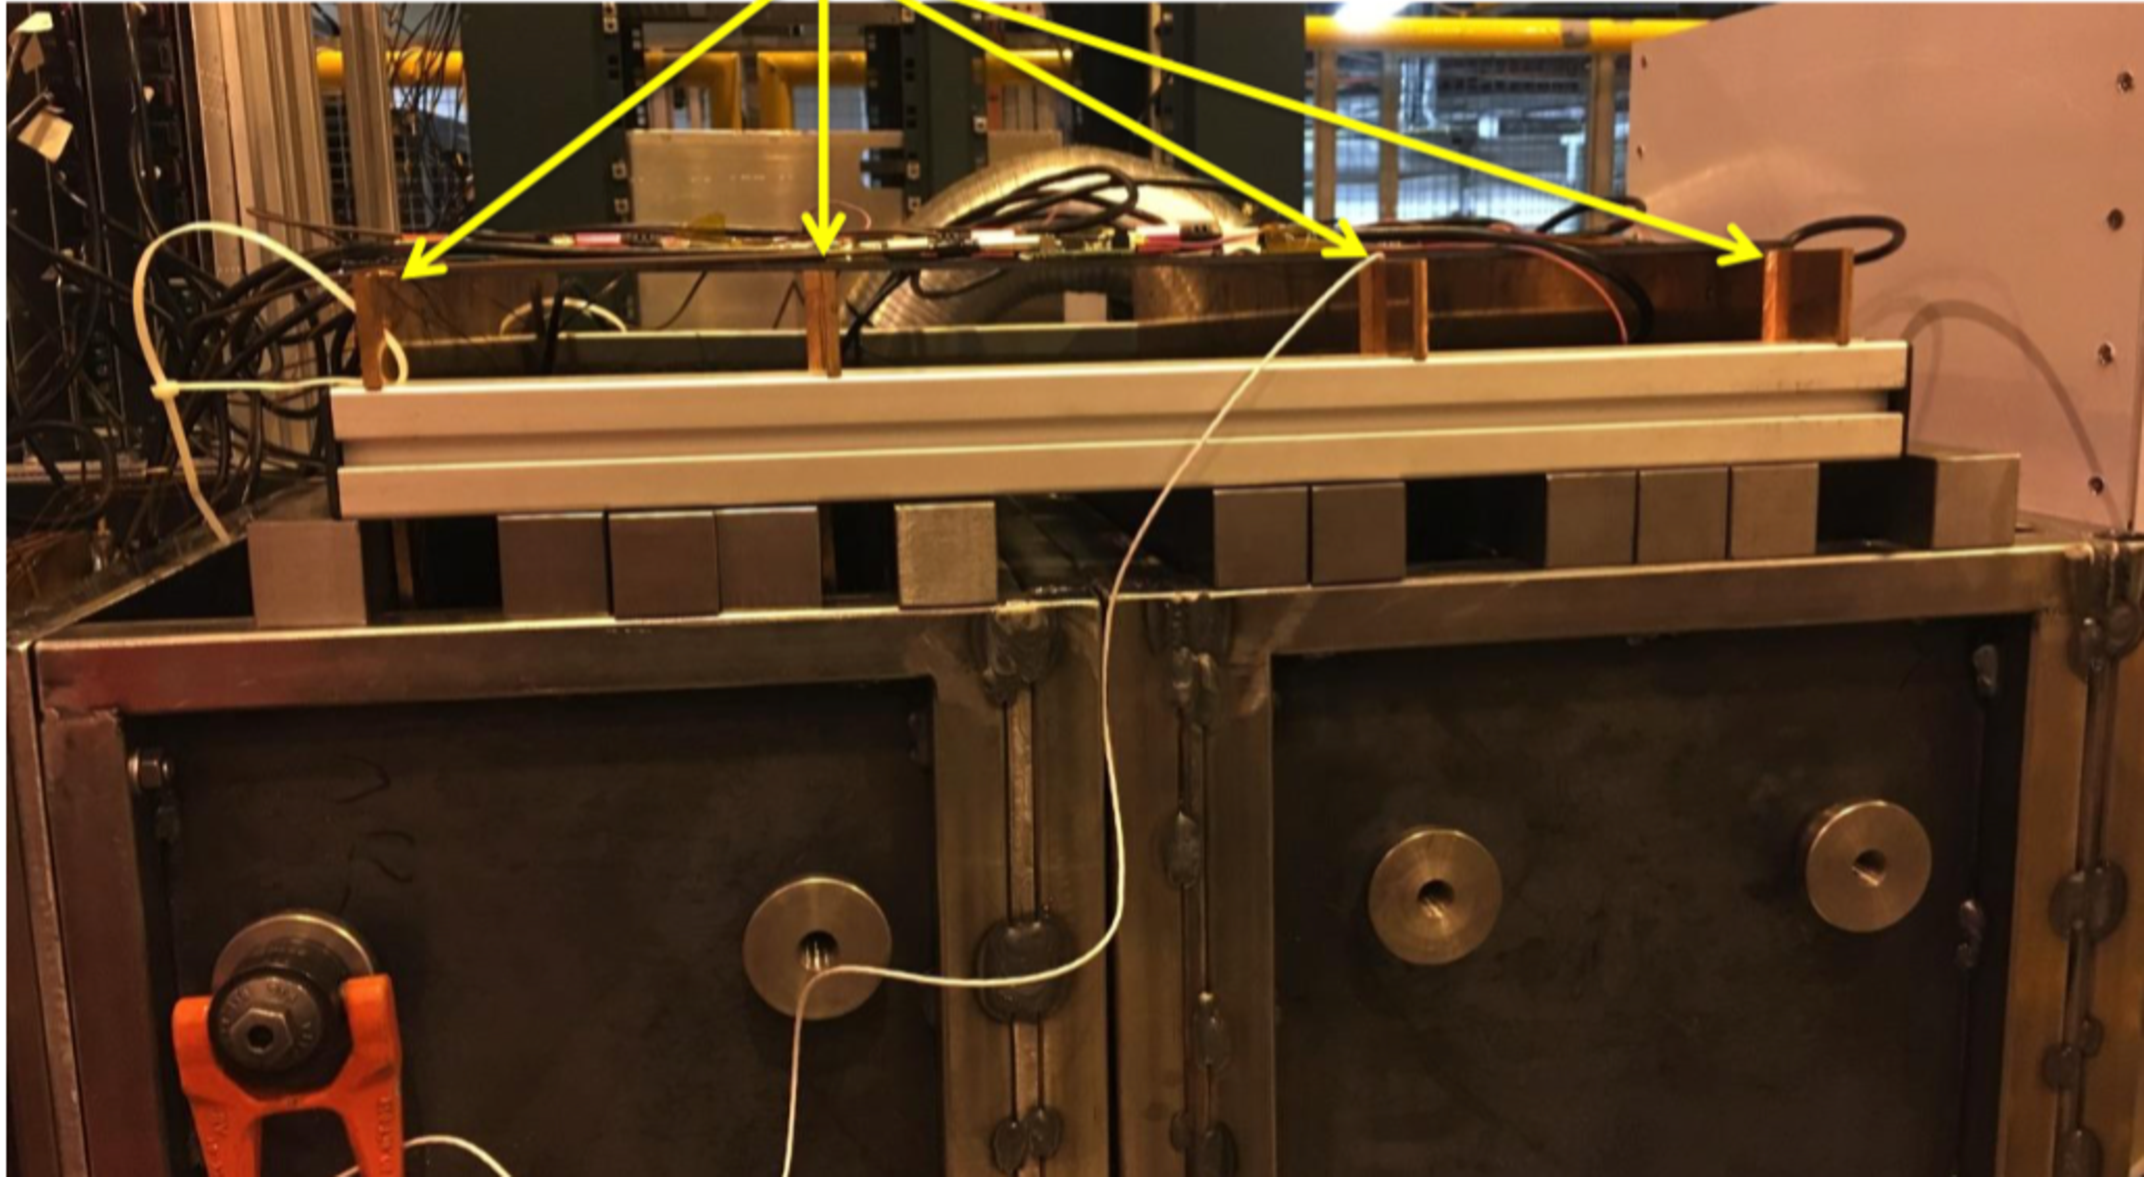
\includegraphics[width=.7\textwidth]{figures/2017JulyTestBeam_FH_position.pdf}
\caption{The movable position of 4 FH modules}
\label{pics:blablabla}
\end{figure}

\begin{figure}
\centering
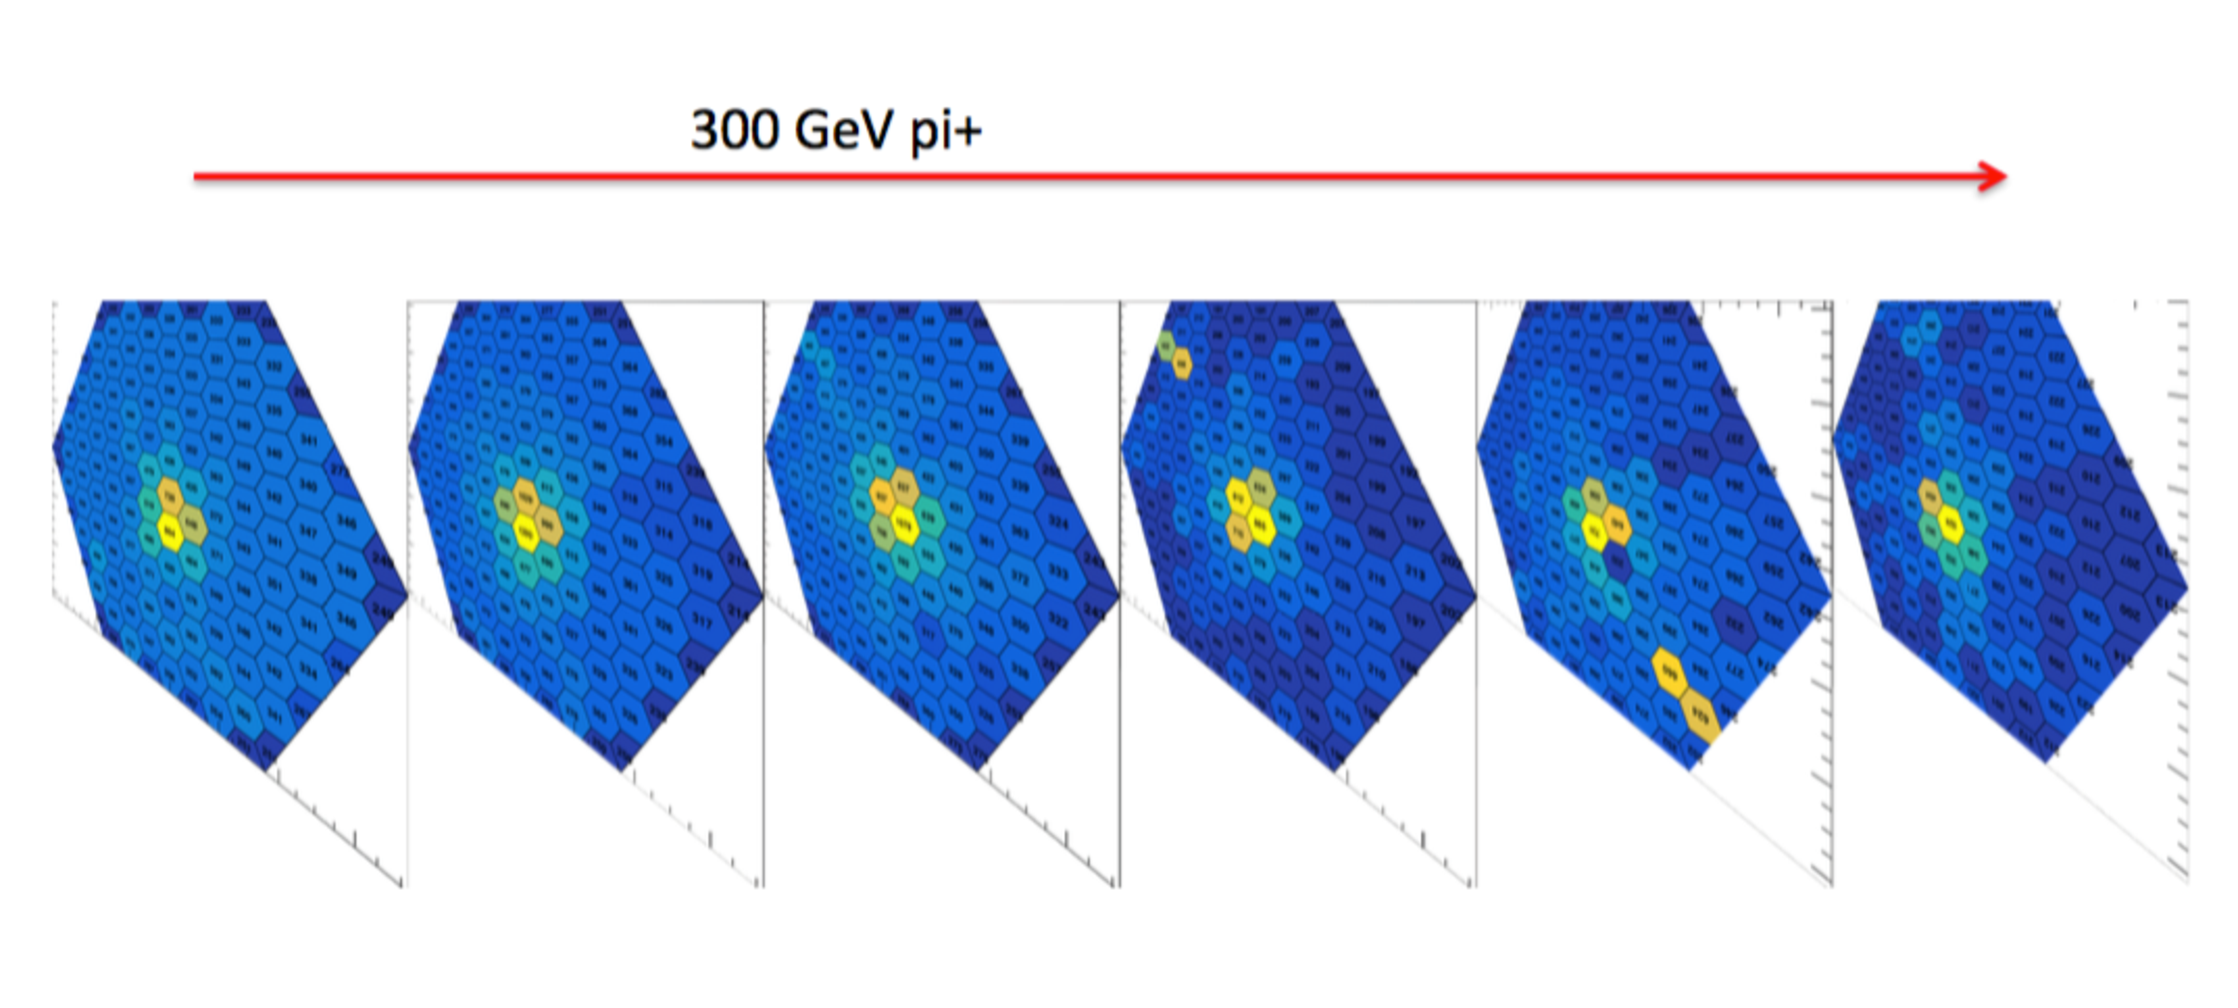
\includegraphics[width=.7\textwidth]{figures/2017JulyTestBeam_eventDisplay.pdf}
\caption{An event display of 300 GeV pion beam. The FH part only shows the hexaboards on the center. The 4-the and the 5-th hexaboard have high noise in the edge where the HDMI cable connectes}
\label{pics:blablabla}
\end{figure}

\begin{figure}
\centering
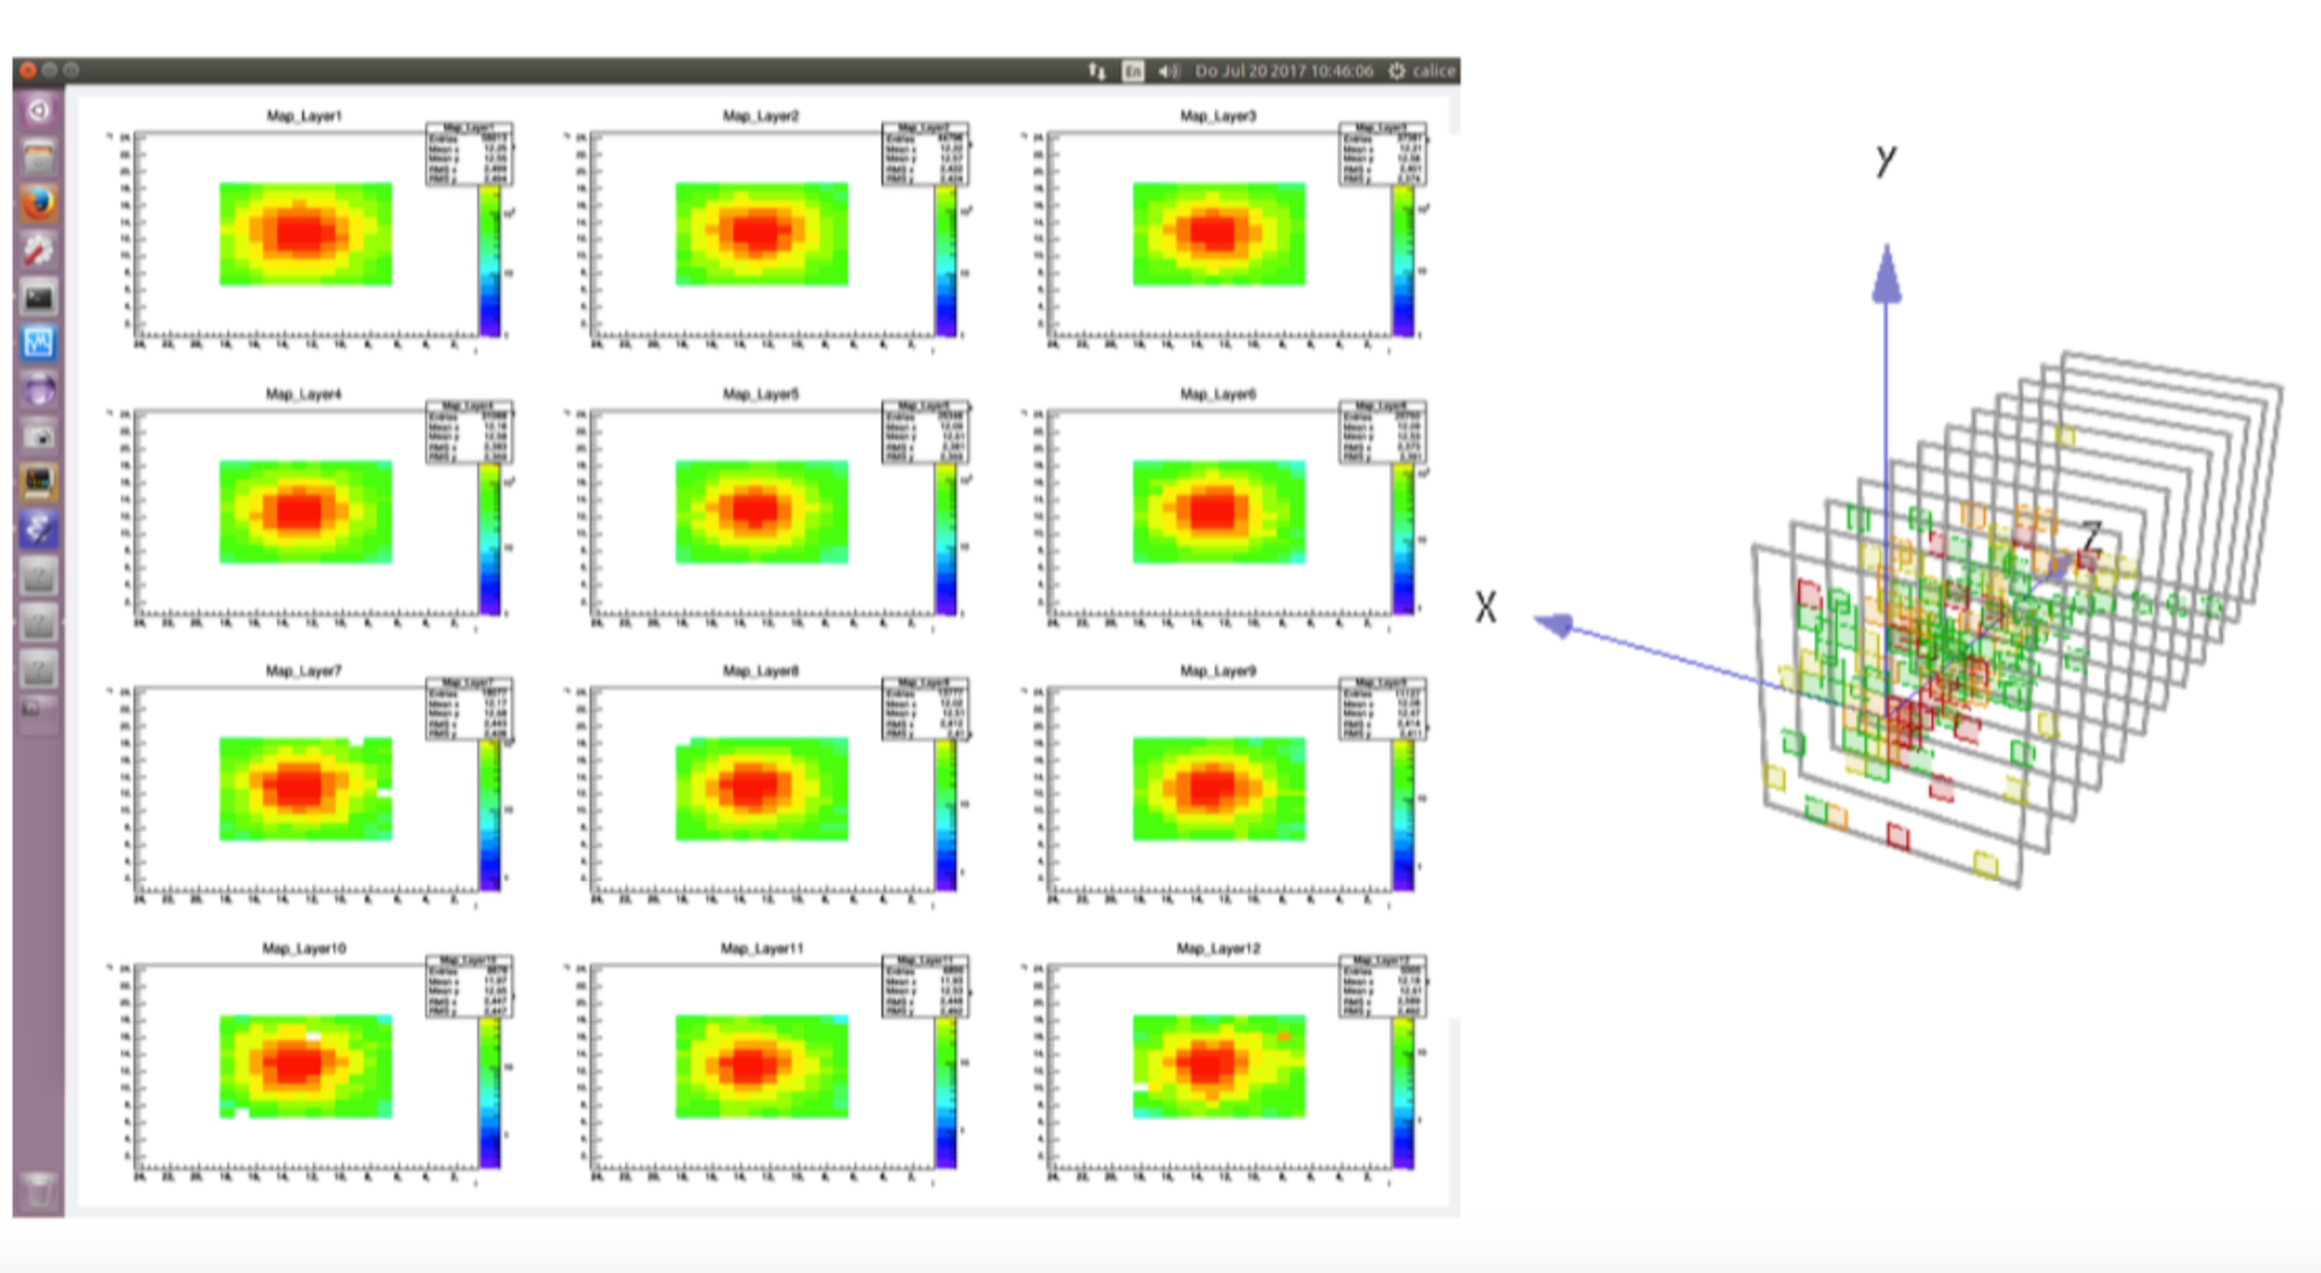
\includegraphics[width=.7\textwidth]{figures/2017JulyTestBeam_AHCAL_DataTaking.pdf}
\caption{AHCAL data-taking monitoring}
\label{pics:blablabla}
\end{figure}



\section{Service task for JMAR group}


In June and Juky I worked for a task for the Jet MissingET Algorithm Reconstruction (JMAR) group as the service work, which was to adding few genjet energy fraction variables to the current CMSSW code, because they were missing in current code. The variables that I added were the charged EM energy, the neutral EM energy, the charged hadron energy and the neutral hadron energy, and I used the particle ID to classify each generator-level particles composed the genjet and then summed their energy to the corresponding energy variables. My github code can be found in \cite{JETMET my git code}.  

Also I produced a private TTbar sample to validate the task. Figure 24 shows the four variables. Figure 25 shows the variables in the RECO-level v.s generator-level, where three variables look linear but the neutral hadron energy does not, which is mainly caused by the definition of the RECO-level neutral hadron energy in CMSSW code doesn't contain the electromagnetic calorimeter(ECAL) energy whereas the generator-level one does.  

Figure 26 shows the averaged energy fraction in the TTbar sample. The lepton cleaning (remove the genjet overlapped with the leptons from the W boson in its cone size) had been implemented. The rest lepton fraction was caused by the lepton decayed from the hadronization of the b-quark.  

This result has been represented in the JMAR meeting and the XPOG meeting. Now I am waiting for the pull request to merged my code to current CMSSW code.


\begin{figure}
\centering
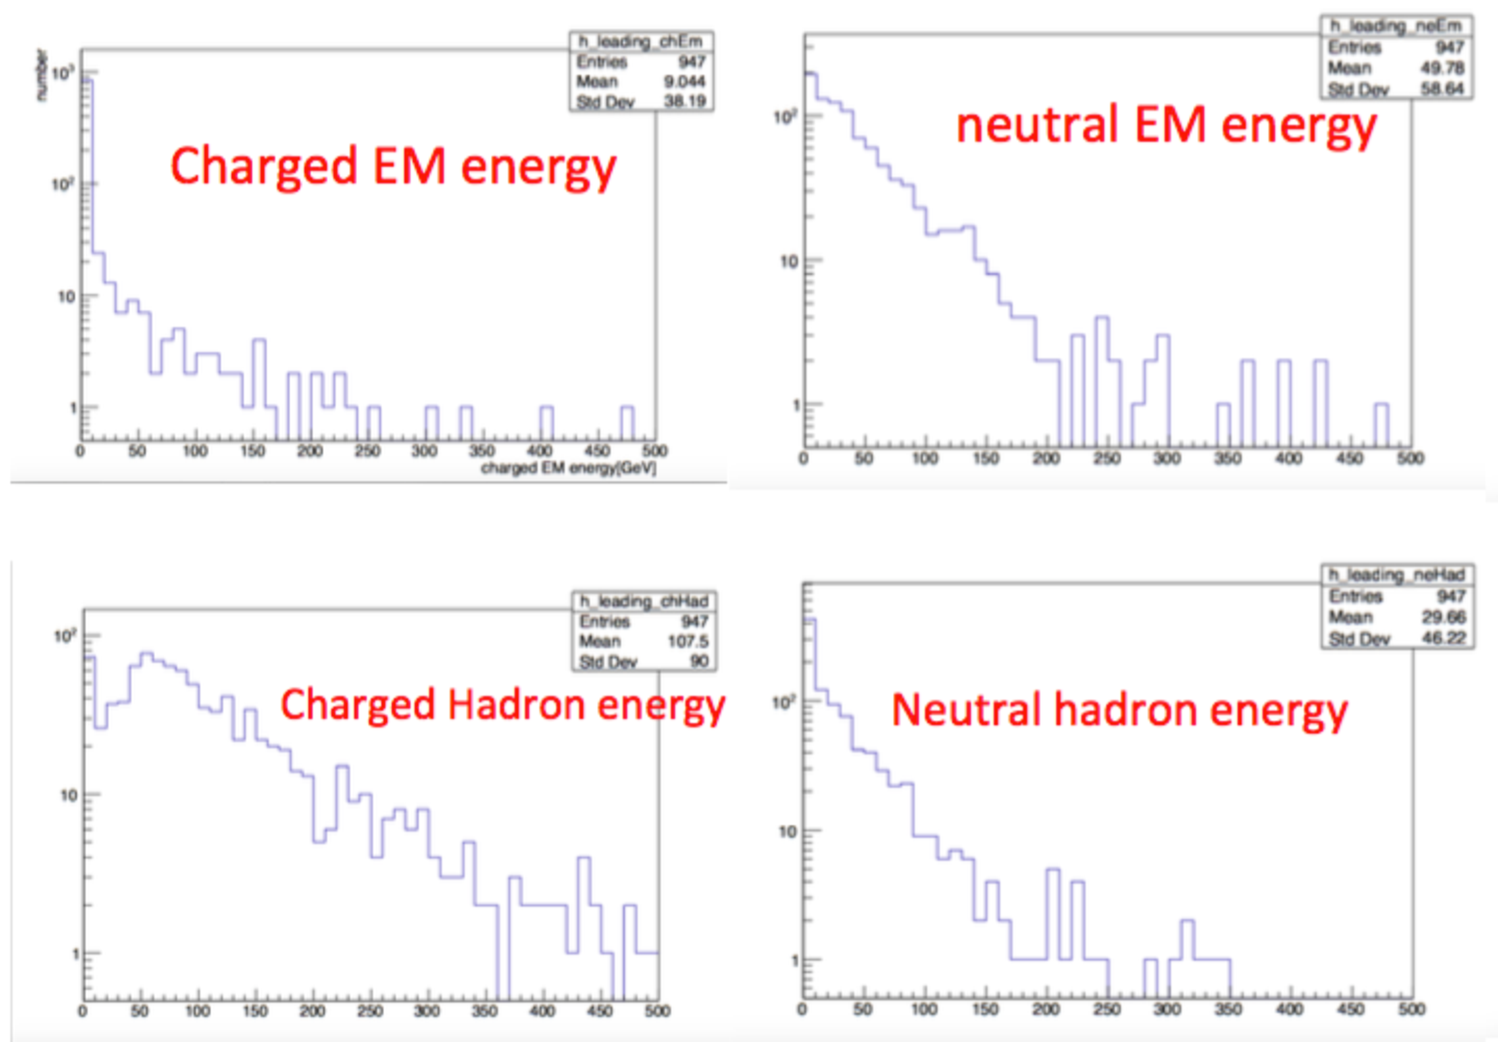
\includegraphics[width=.7\textwidth]{figures/genjet_variables.pdf}
\caption{the distribution of the charged EM energy(top left), the neutral EM energy(top right), the charged hadron energy(bottom left), and the charged EM energy(bottom right). The y-axes are in log scale}
\label{pics:blablabla}
\end{figure}

\begin{figure}
\centering
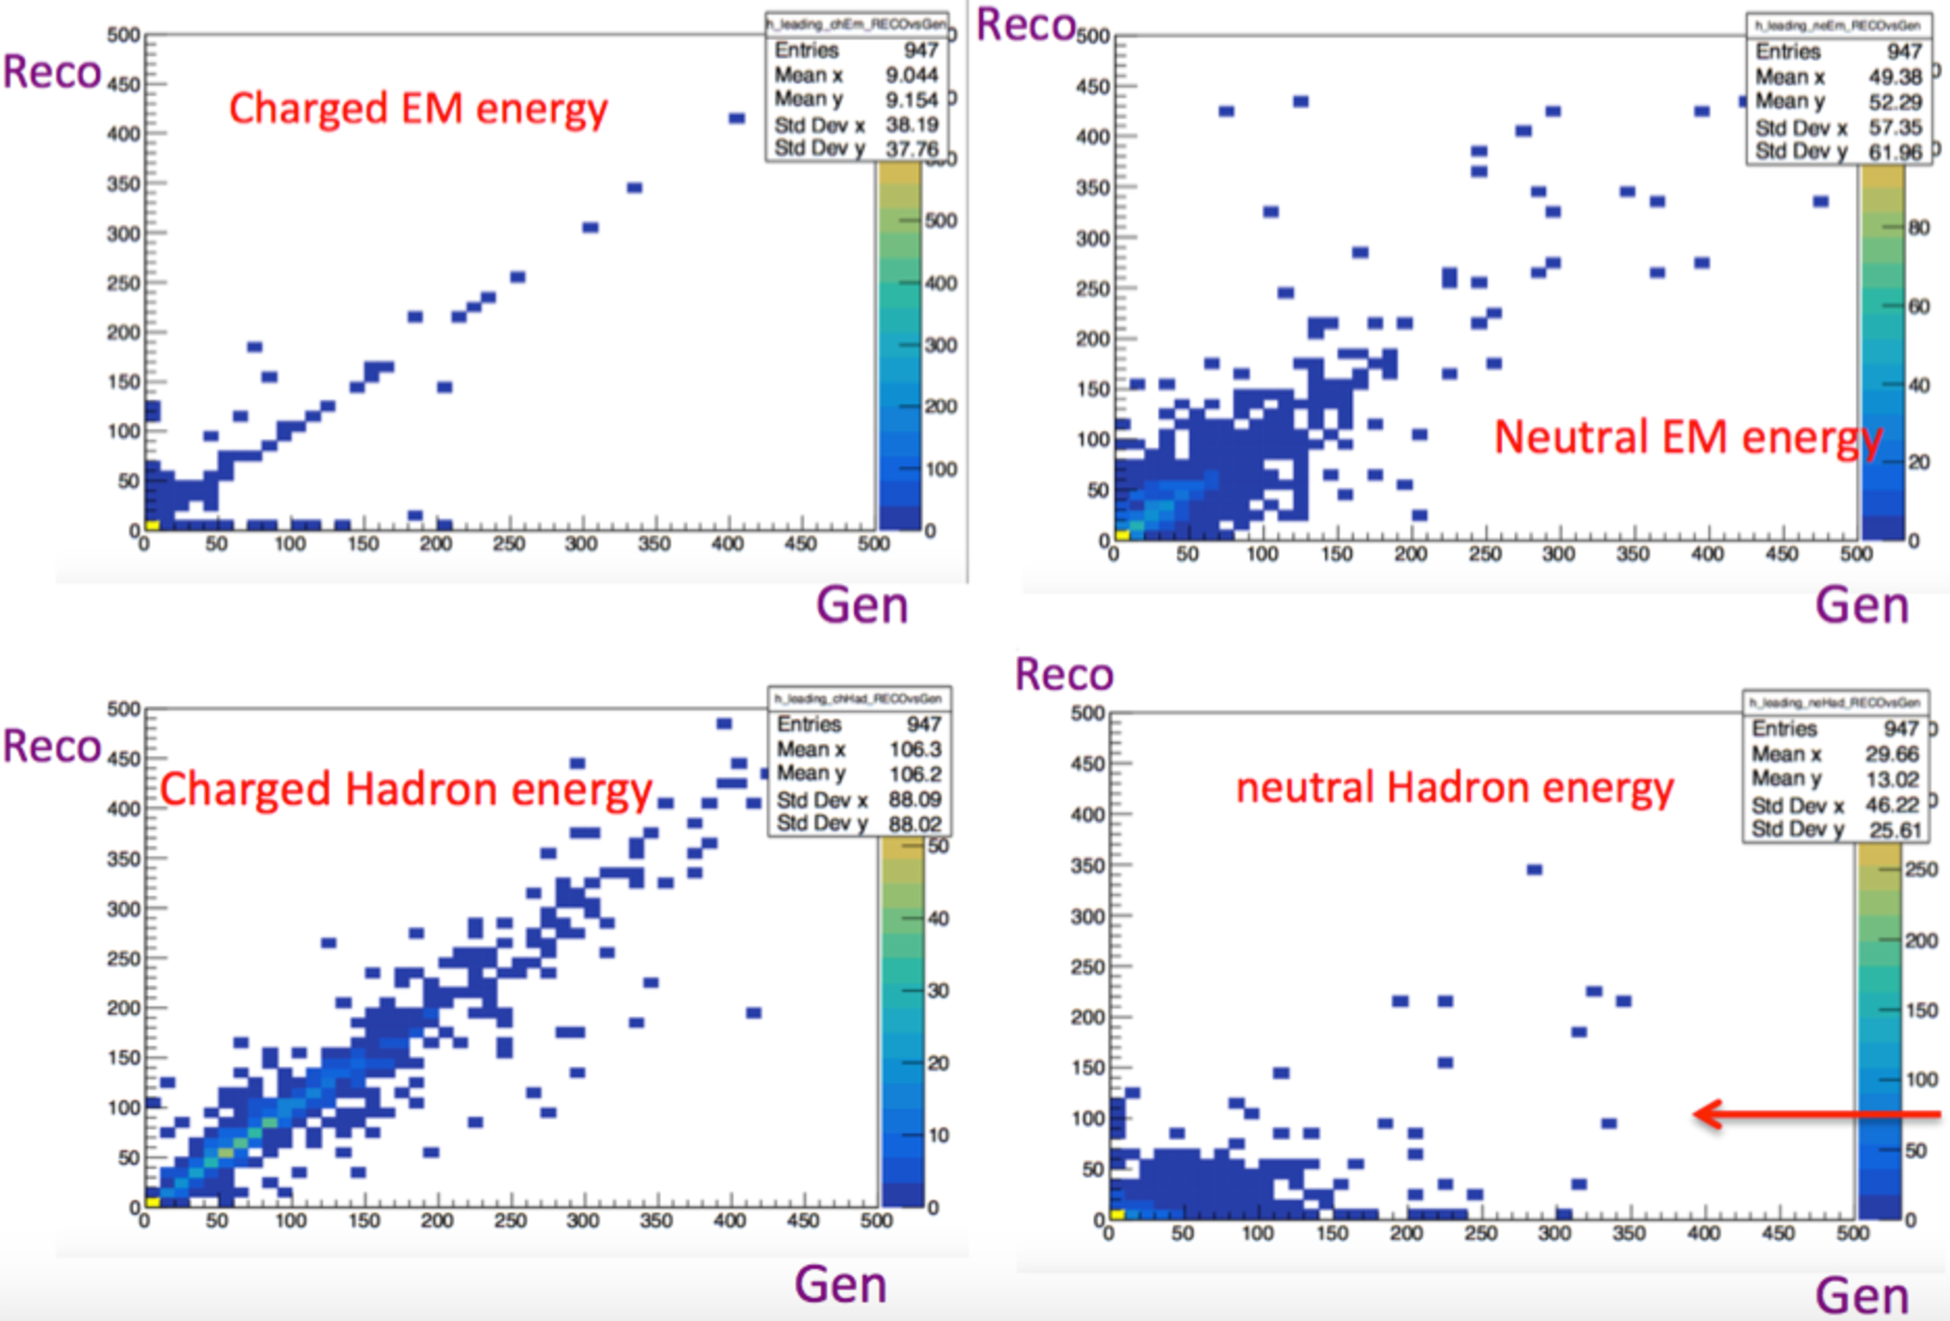
\includegraphics[width=.7\textwidth]{figures/genjet_variables_RecovsGen.pdf}
\caption{the RECO-level v.s the generator-level 2D distribution of the charged EM energy(top left), the neutral EM energy(top right), the charged hadron energy(bottom left), and the charged EM energy(bottom right.}
\label{pics:blablabla}
\end{figure}

\begin{figure}
\centering
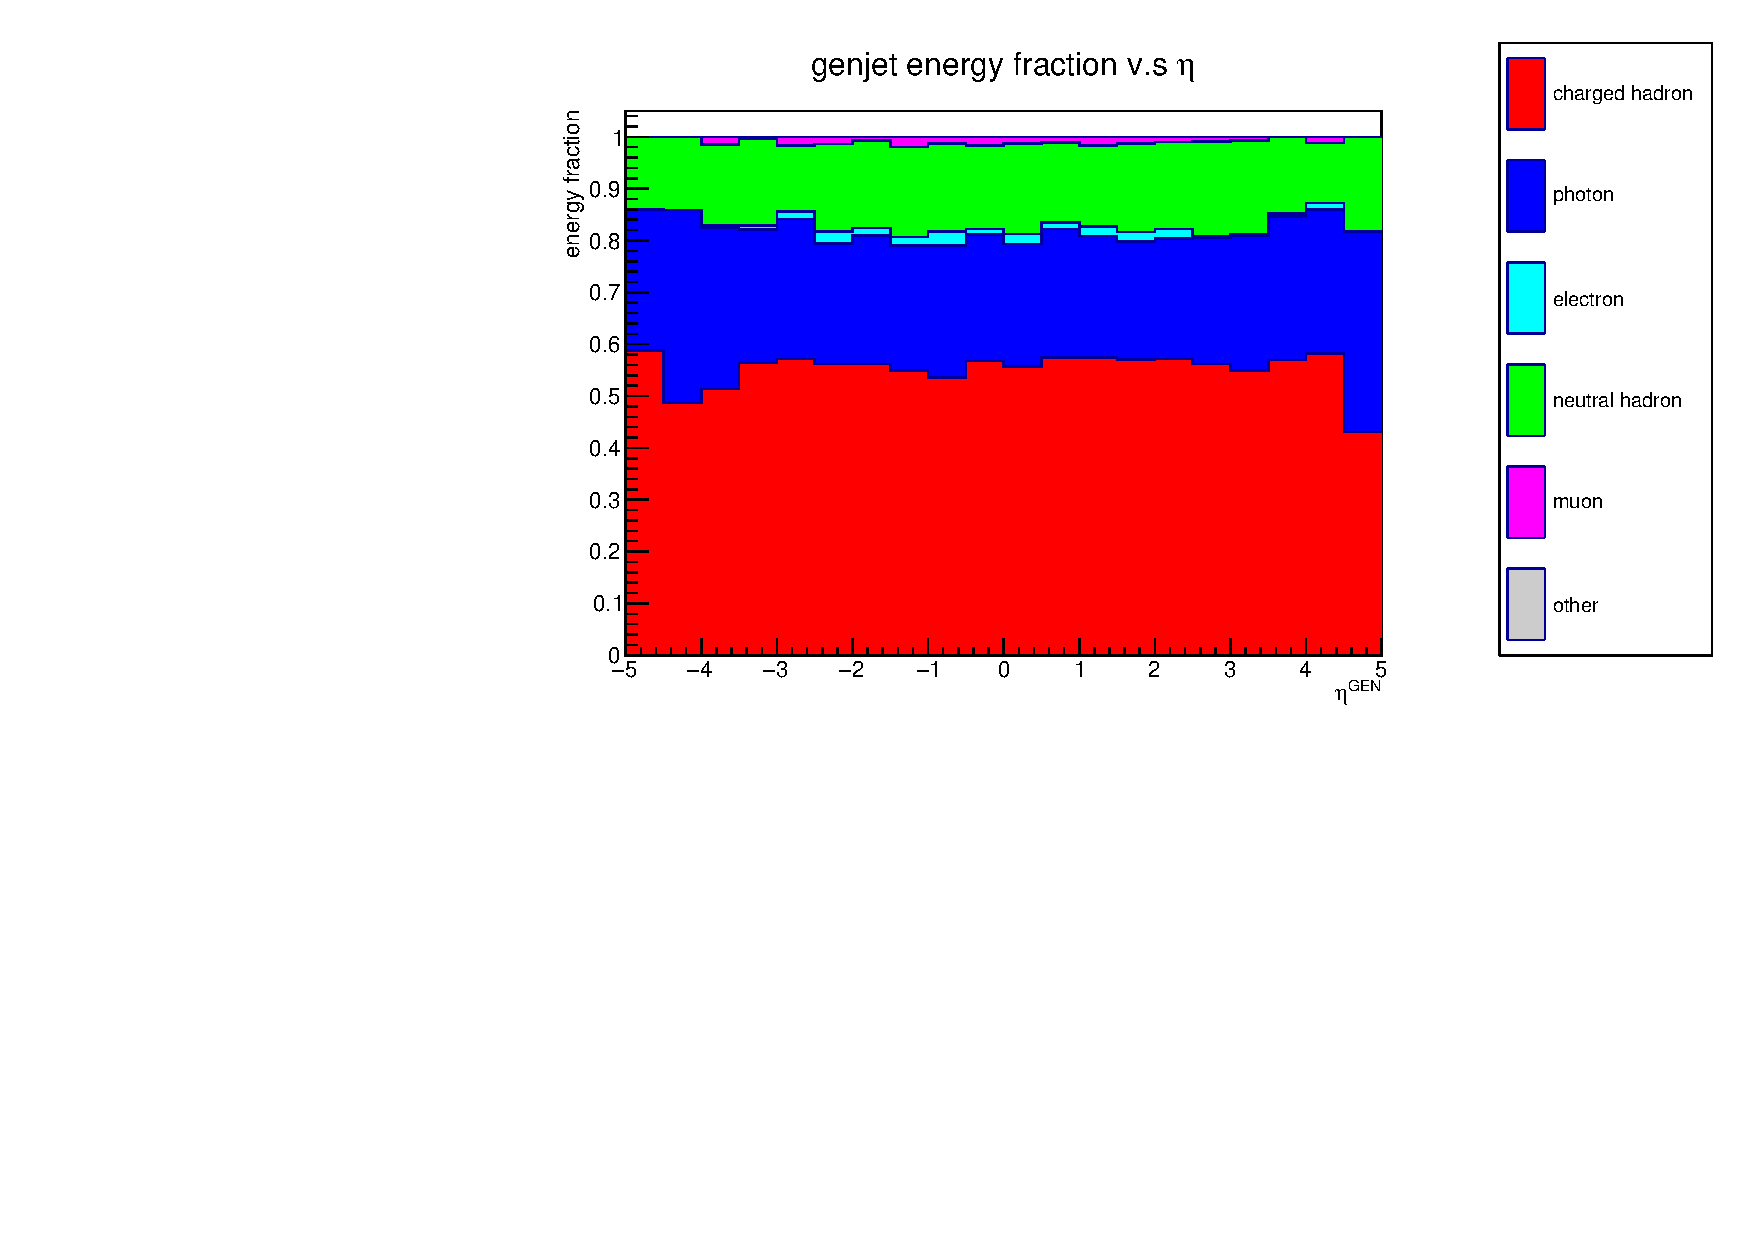
\includegraphics[width=1.\textwidth]{figures/genjet_energy_fraction_20Bins.pdf}
\caption{The averaged genjet energy variable fraction v.s $\eta$. The Sum of all energy fractions equals to unty by the definition.}
\label{pics:blablabla}
\end{figure}



\section{CMS trigger shift for 2017 data taking}

During March to June 2017, I took the trigger shifts of the Compact Muon Solenoid(CMS) experiment. The trigger system is used to reduce the rate of data-taking and only select the event that people are interest. In CMS, the trigger is composed by the level-1 trigger (L1) and the high-level trigger (HLT), where the L1 is the hardware-based trigger to reduce the rate \textless  100 kHz by basic thresholds and the HLT is the computer-farm based trigger to subsequently reduce the rate \textless 1 kHz by the algorithms. All L1 subsytems used in 2017 are shown in Figure 27. 

The trigger shifter's role is to cooperate with other crews in the CMS control room (in building 3562 or SCX5) located at the LHC Point5 when the CMS is in operation. The trigger shifter need to make sure the triggers in use working well (function ok and has resonable rate), comunicate with other crews when error happens, change the pre-scale column, which decide differnt pre-scale number for different trigger, to suppress total rate according to the current luminosity, and upload a shift report to the Elog in the end of the shift. The seats and photo of trigger shift are shown in Figure 28 and Figure 29, and the trigger L1-page, which is the one of the most frequently used interfaces, is shown in Figure 30.   

In totally I took 15 shifts and get 19 credits for the NCU institue, and each shift took 8 hours (11-7,7-15 or 15-23).

\begin{figure}
\centering
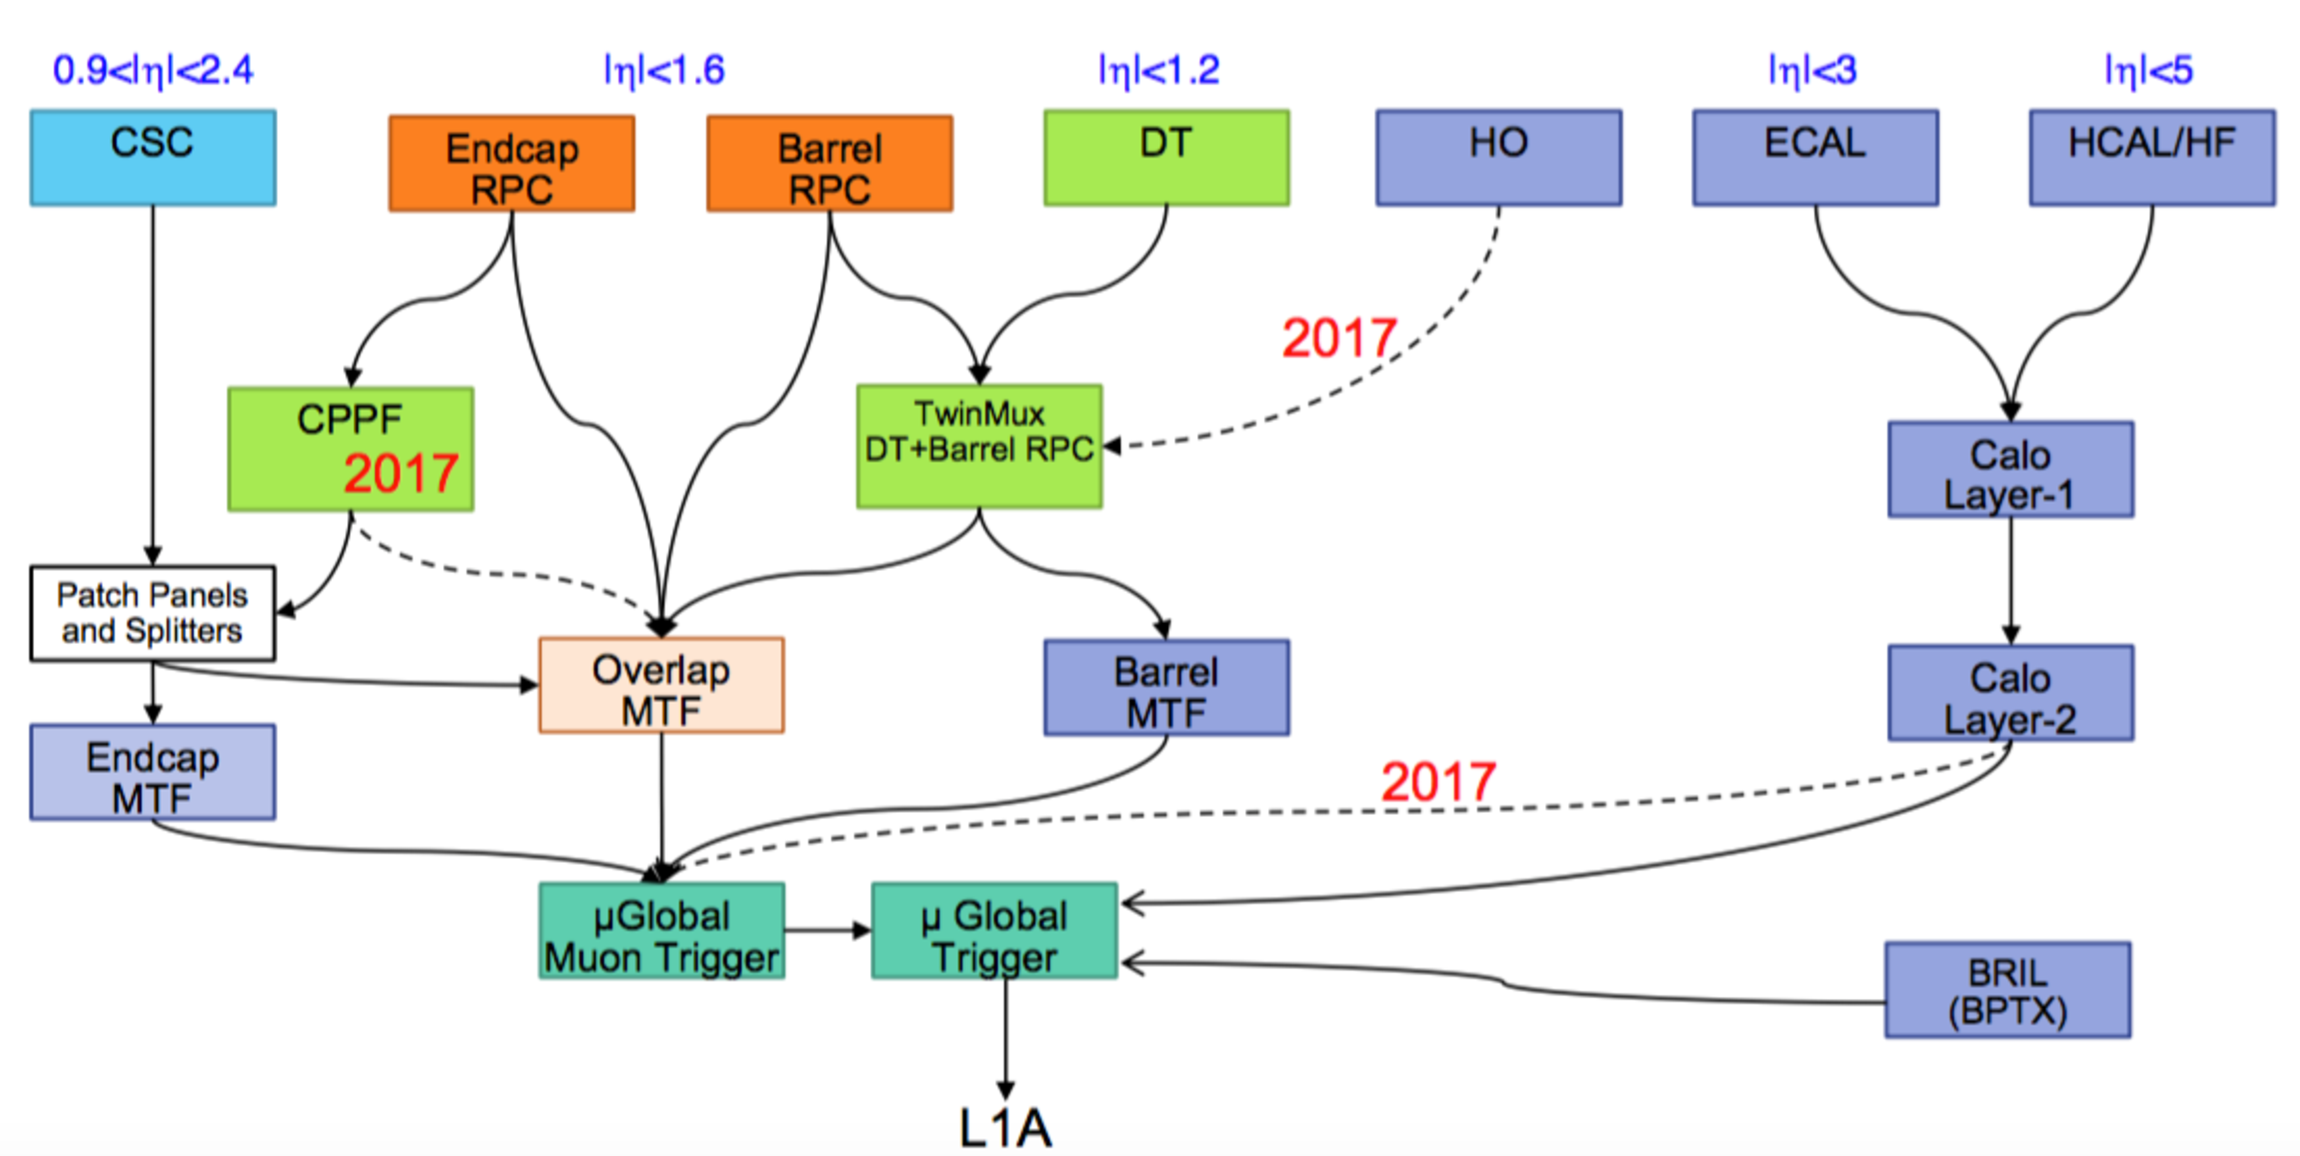
\includegraphics[width=1.\textwidth]{figures/TriggerShift_subsystem.pdf}
\caption{The level-1 trigger subsystem in 2017}
\label{pics:blablabla}
\end{figure}

\begin{figure}
\centering
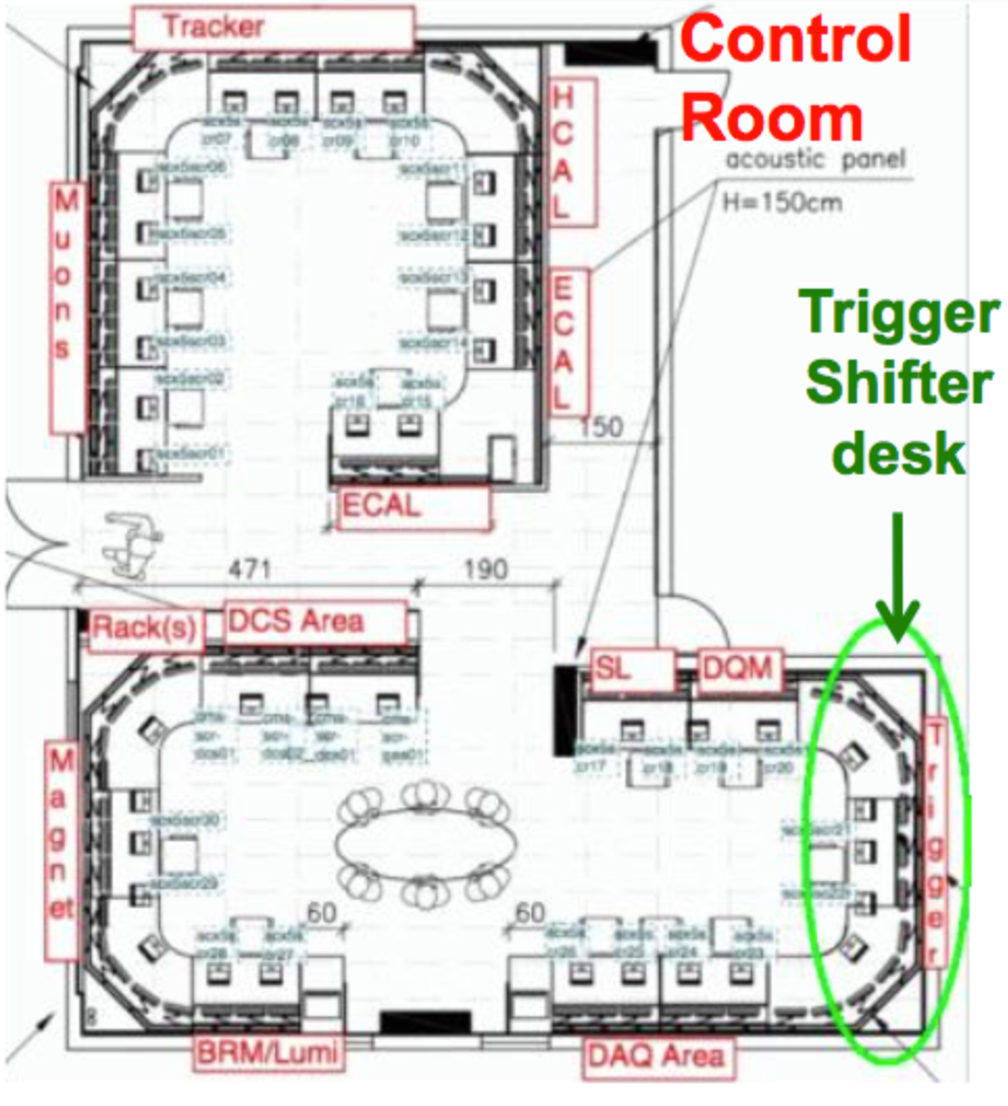
\includegraphics[width=.7\textwidth]{figures/TriggerShift_seat.pdf}
\caption{The seats of the CMS control room}
\label{pics:blablabla}
\end{figure}

\begin{figure}
\centering
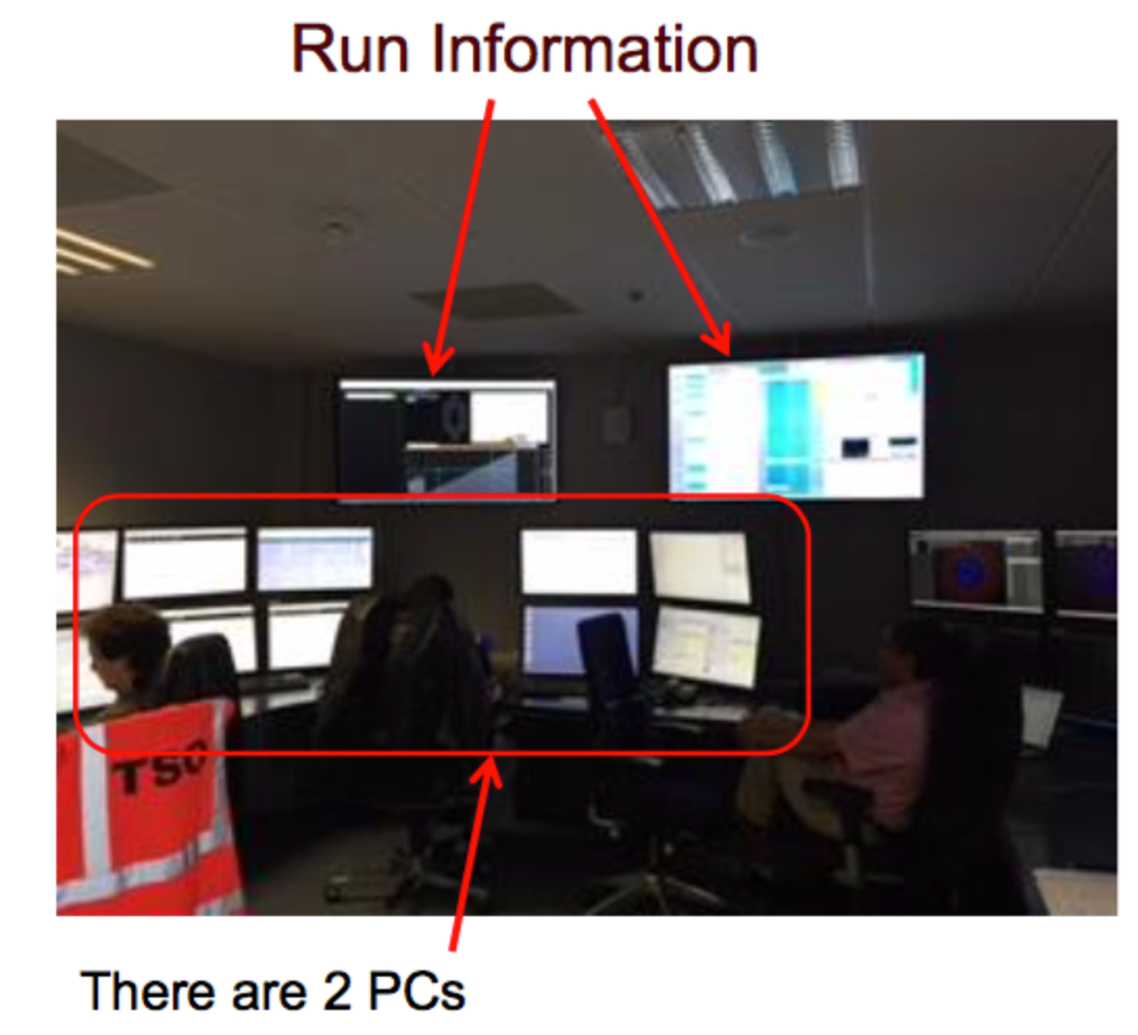
\includegraphics[width=.7\textwidth]{figures/TriggerShift_photo.pdf}
\caption{Photo of trigger shifter's seat. Two PCs with 4 screen per PC for the DQM shifter(left) and trigger shifter(right)}
\label{pics:blablabla}
\end{figure}

\begin{figure}
\centering
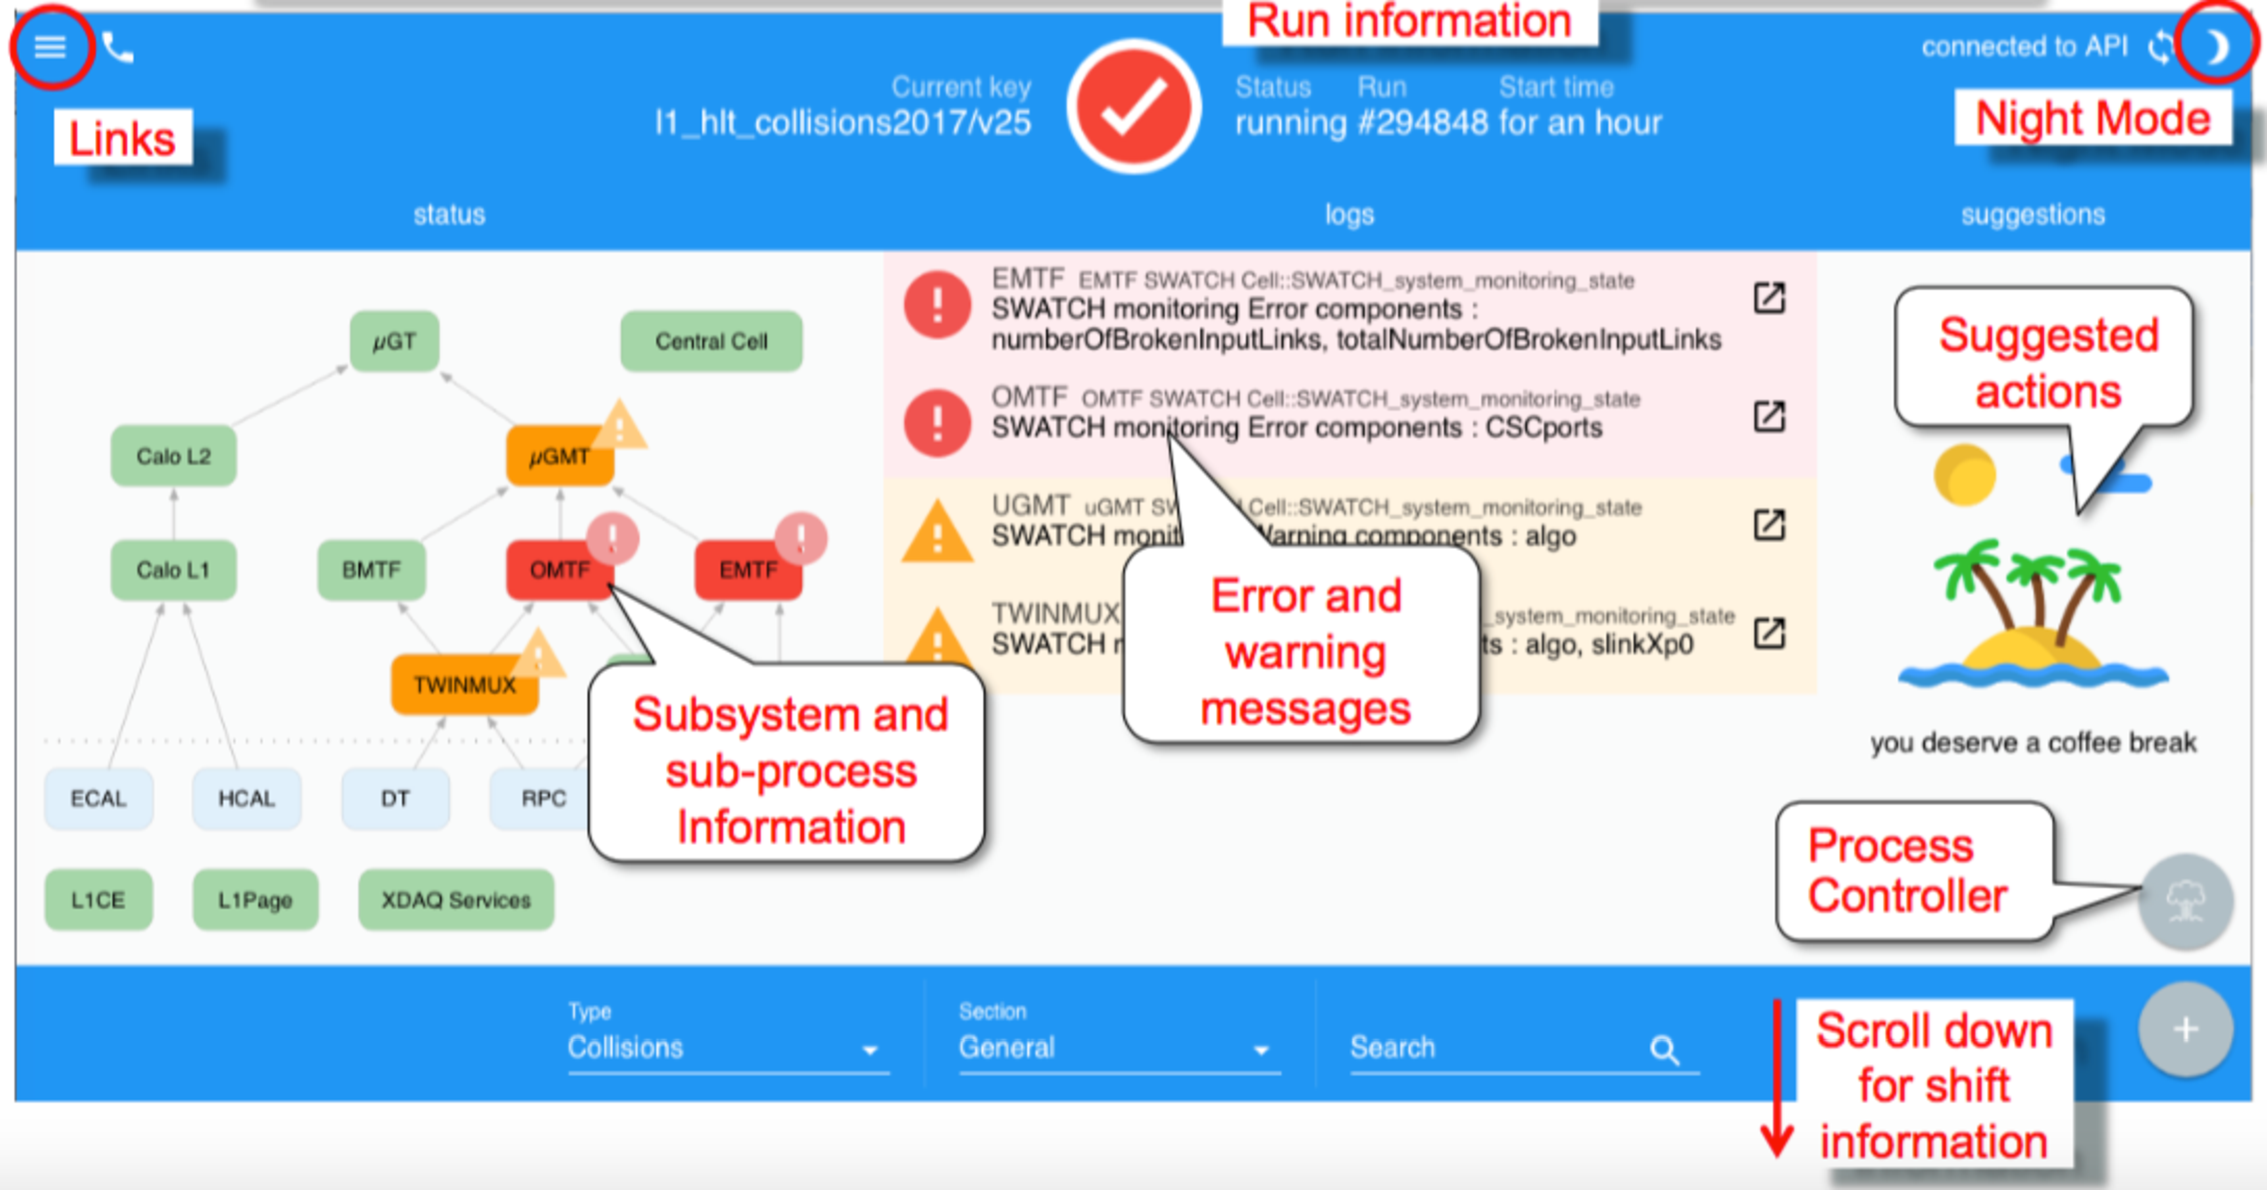
\includegraphics[width=1.\textwidth]{figures/TriggerShift_interface.pdf}
\caption{The trigger L1-page interface}
\label{pics:blablabla}
\end{figure}


%\end{comment}

\newpage
%
% ---- Bibliography ----
%


\begin{thebibliography}{9}

\bibitem {Alberto ZH paper with 2015 data}
CMS Collaboration, ``Search for heavy resonances decaying into a vector boson and a Higgs boson in final states with charged leptons, neutrinos, and b quarks'',CERN, 2016.\\
\url{https://arxiv.org/abs/1610.08066}

\bibitem {double B-tagger paper}
CMS Collaboration, ``Identification of double-b quark jets in boosted event topologies'', CERN, 2016.\\
\url{https://cds.cern.ch/record/2195743}

\bibitem {double B-tagger SF twiki}
CMS internal twiki link, ``Usage of b/c Tag Objects for 13 TeV Data in 2016 and 80X MC''.\\
\url{https://twiki.cern.ch/twiki/bin/viewauth/CMS/BtagRecommendation80XReReco}

\bibitem {HGCal ref}
CMS Collaboration, ``CMS Forward Calorimeters Phase II Upgrade'', CERN, 2014.\\
\url{https://cds.cern.ch/record/1969369}

\bibitem {DN-17-011}
CMS internal twiki link, ``Paper Summarising 2016 Beam Tests at FNAL and CERN'',2017.\\
\url{https://twiki.cern.ch/twiki/bin/viewauth/CMS/BeamTestPaper2016}

\bibitem {May 2017 TB google doc}
Google doc for 2017 May test beam data.\\
\url{https://docs.google.com/spreadsheets/d/1ju1r2Be2dpvIa7_QnCeufZ9UqPE1CeJrtBJivwTI68U/edit#gid=0}

\bibitem {CALICE ref}
Home page of the CALICE experiment.\\
\url{https://twiki.cern.ch/twiki/bin/view/CALICE/WebHome}

\bibitem {July 2017 TB google doc}
Google doc for 2017 July test beam data.\\
\url{https://docs.google.com/spreadsheets/d/1ZUL7VM7EK651mL_FGNUkcBkE0tJtqkRVMfAqTUYqt7g/edit#gid=91437087} 

\bibitem {JETMET my git code}
My github repository forked for the JMAR task\\
\url{https://github.com/yuchanggit/cmssw/blob/master/RecoJets/JetProducers/src/JetSpecific.cc}\\
\url{https://github.com/yuchanggit/cmssw/blob/master/DataFormats/JetReco/interface/GenJet.h}

\end{thebibliography}

\end{document}
